\documentclass[aps,prx,reprint,superscriptaddress,floatfix,nofootinbib,longbibliography,amsmath,amssymb]{revtex4-2}
\usepackage[T1]{fontenc}
\IfFileExists{lmodern.sty}{\usepackage{lmodern}}{}
\usepackage{amsthm,mathtools}
\usepackage{enumitem}
\usepackage{booktabs,array}
\usepackage{xcolor}
\usepackage{tenkz}
\usetikzlibrary{quantikz2}
\usetikzlibrary{arrows.meta,calc,patterns,positioning,decorations.pathreplacing}
\usepackage{graphicx,adjustbox}
\usepackage[colorlinks=true,linkcolor=blue!50!black,citecolor=blue!50!black,urlcolor=blue!50!black]{hyperref}

% ---------- notation ----------
\newcommand{\C}{\mathbb C}
\newcommand{\R}{\mathbb R}
\newcommand{\Z}{\mathbb Z}
\newcommand{\E}{\mathbb E}
\newcommand{\id}{\mathrm{I}}
\newcommand{\Tr}{\operatorname{Tr}}
\newcommand{\dist}{\operatorname{dist}}
\newcommand{\supp}{\operatorname{supp}}
\newcommand{\rank}{\operatorname{rank}}
\newcommand{\diam}{\operatorname{diam}}
\newcommand{\norm}[1]{\lVert #1\rVert}
\newcommand{\abs}[1]{\lvert #1\rvert}
\providecommand{\ket}[1]{|#1\rangle}\renewcommand{\ket}[1]{|#1\rangle}
\providecommand{\bra}[1]{\langle #1|}\renewcommand{\bra}[1]{\langle #1|}
\newcommand{\cH}{\mathcal H}
\newcommand{\cB}{\mathcal B}
\newcommand{\cE}{\mathcal E}
\newcommand{\cI}{\mathcal I}
\newcommand{\cR}{\mathcal R}
\newcommand{\cV}{\mathcal V}
\newcommand{\cT}{\mathcal T}
\newcommand{\cA}{\mathcal A}
\newcommand{\cF}{\mathcal F}
\newcommand{\cS}{\mathcal S}
\newcommand{\cQ}{\mathcal Q}
\newcommand{\cK}{\mathcal K}
\newcommand{\Om}{\Omega}
\newcommand{\Lam}{\Lambda}
\newcommand{\e}{\mathrm e}

\theoremstyle{plain}
\newtheorem{theorem}{Theorem}[section]
\newtheorem{proposition}[theorem]{Proposition}
\newtheorem{lemma}[theorem]{Lemma}
\newtheorem{corollary}[theorem]{Corollary}
\theoremstyle{definition}
\newtheorem{definition}[theorem]{Definition}
\newtheorem{remark}[theorem]{Remark}
\newtheorem{construction}[theorem]{Construction}

% ---------- parts (REVTeX has no \part) ----------
\newcounter{notepart}
\renewcommand{\thenotepart}{\Roman{notepart}}
\newcommand{\notepart}[2]{\refstepcounter{notepart}\label{#2}%
  \par\medskip\noindent{\centering\large\bfseries Part~\thenotepart\\[2pt]#1\par}\medskip}

% ---------- the "written twice" device ----------
% Every mathematical unit of this note appears twice: first in words
% (what it says, why it is true, what it is for), then precisely.
\newenvironment{inwords}{%
  \par\medskip\noindent
  \begin{list}{}{\leftmargin=0.8em\rightmargin=0.8em}
  \item\relax
  \noindent{\sffamily\bfseries\color{blue!40!black}In words.}\ \sffamily\small}{%
  \end{list}\par\medskip}
\newcommand{\precisely}{\par\noindent{\bfseries Precisely.}\ }

\begin{document}

\title{A one-dimensional area law and a matrix product state
approximation from a global spectral gap: the collar-free route}
\author{Prepared for Sirui Lu}
\affiliation{Max Planck Institute of Quantum Optics, Garching}
\date{October 16, 2026}

\begin{abstract}
\noindent
We prove an entanglement area law and a polynomial matrix product state
approximation for the unique gapped ground state of any finite-range
one-dimensional Hamiltonian, specialising the two-dimensional arguments
of \emph{A two-dimensional area law from a global spectral gap} \cite{AL}
and \emph{Polynomial PEPS approximation of gapped square-grid ground
states} \cite{PP} to a spin chain. Two structural simplifications occur on
a line. First, the area-law proof collapses to three elementary steps: the
marginal tail bound and the buffered conditional-entropy discount of
\cite[Section~2]{AL}, combined with the Araki--Lieb inequality, directly
yield $S(X)\le C(q,R)\,(1+J/\Delta)$ for every interval $X$. The
reason is geometric: a shell around an interval is crossed by a bounded
number of interactions, so the conditional-entropy discount costs a
constant rather than a boundary-scaled error, and the
buffer whose entropy must be controlled contains only a constant number of
sites. The sub-volume recursion, positive quasi-local constraints, replica
scanner, amplification, and two-family geometry of \cite{AL} drop out
entirely. Second, the tensor-network construction reduces from a dyadic
hierarchy to a linear left-to-right \emph{sweep}. The encoded holes,
adaptive patch constraints, angular information estimates, and row--column
routing of \cite{PP} disappear; what remains are Uhlmann-type birth,
death, and exchange moves, an information reset via a two-sided Gaussian
spectral filter, dimension-free Gaussian density compression, and column
extraction. The output is a matrix product state of bond dimension
$CL^{c}$ within vector error $L^{-1}$ of the ground state. We also record
that in one dimension the marginal tail bound makes the matrix product
state theorem a two-line corollary of the area law by sequential Schmidt
truncation. Every statement in this note is written twice: first in words,
then precisely. The area-law proof uses none of the techniques of Hastings
or of Arad--Kitaev--Landau--Vazirani; the tensor-network protocol uses a
Lieb--Robinson bound in a single lemma, and we indicate how to avoid it at
the price of a quasi-polynomial bond dimension.
\end{abstract}
\maketitle



\section{Overview}

\begin{inwords}
In a gapped quantum lattice system, entanglement across a region is
generated along its boundary. In two dimensions, a region of linear size
$r$ has a boundary of $O(r)$ sites: every variational estimate across the
boundary incurs an $O(r)$ error, and any buffer introduced to isolate the
region is an annulus whose own entanglement is unknown. The multi-scale
replica, scanner, and amplification apparatus of \cite{AL} exists to
break this circularity. In one dimension, the boundary of an interval is at
most two points. Any variational operation across the boundary disturbs a
bounded number of interactions and costs $O(1)$ energy, while a buffer of
constant width has, trivially, constant entropy. The circularity never arises: a marginal tail bound,
a buffered conditional-entropy discount, and the Araki--Lieb inequality
establish the area law in full. This is the content of
Part~\ref{part:arealaw}.

Constructing a global tensor-network approximation requires more than
entropy bounds alone (the papers explain why: an entropy bound on each cut
does not give a global vector approximation).
The two-dimensional construction of \cite{PP} therefore distributes the
ground state among ``parties'' attached to dyadic squares via local
changes of ownership controlled by mutual information, and then compresses
the resulting distributed density operator into a tensor network. On a
line, a dyadic hierarchy is the wrong geometry: a binary tree of intervals
has cutwidth $\log L$ across the middle of the chain, which turns a
polynomial link dimension into a quasi-polynomial bond dimension. The
right geometry is a left-to-right sweep with a moving ``remainder'' party,
which keeps the cutwidth bounded. The only topological obstruction during
the sweep is dissolving a narrow remainder band wedged between two
distinct neighbouring owners; this is resolved by the same sequence of
Uhlmann birth, death, and two-sheet exchange moves used along block edges
in \cite{PP}. This is Part~\ref{part:mps}. We also show that, in one
dimension, the marginal tail bound of Part~\ref{part:arealaw} makes the
matrix product state theorem an immediate corollary of the area law by
sequential Schmidt truncation; the sweep protocol is the one-dimensional
counterpart of the two-dimensional construction, and it is the mechanism
that generalises to higher dimensions.

Table~\ref{tab:map} summarises how the two-dimensional architecture
specialises to a line. Readers interested solely in the one-dimensional
area law need only read Sections~\ref{sec:setting}--\ref{sec:closing}
(about four pages).
\end{inwords}

\begin{table*}[t]
\centering\small
\begin{tabular}{@{}p{0.33\textwidth}p{0.63\textwidth}@{}}
\toprule
Two-dimensional ingredient & Specialisation to one dimension\\
\midrule
Marginal tail bound (\cite{AL}, Lemma 2.1) & Kept verbatim; the cut parameter $\mathcal B$ is a constant (Section~\ref{sec:tail}).\\
Buffered conditional-entropy discount (\cite{AL}, Lemma 2.2) & Kept; the buffer has \emph{constant} width and the error is a constant (Section~\ref{sec:buffer}).\\
Sub-volume recursion, exponent $e_0<1$ & Unnecessary: the Araki--Lieb inequality closes the argument directly (Section~\ref{sec:closing}). Sketched for comparison in Section~\ref{sec:longroute}.\\
Positive quasi-local constraints, truncation & Unnecessary for the area law; replaced by the Gaussian filter reset in the MPS protocol.\\
Conditional estimates, replicas, transport, comparators, scanner & Unnecessary.\\
Amplification by random constraint products & Unnecessary; Section~\ref{sec:longroute} explains how it would apply on a line.\\
Two families of regions & Trivial on a half-line; Section~\ref{sec:longroute}.\\
\midrule
Coarse collar and angular information (\cite{PP}, Section 3) & Replaced by a direct consequence of the area law and information reset (Lemma~\ref{lem:logsep}).\\
Information reset by Gaussian filter (\cite{PP}, Lemma 3.3) & Kept with one-dimensional Lieb--Robinson locality (Section~\ref{sec:reset}).\\
Adaptive patch constraints, encoded holes (\cite{PP}, Sections 4, 6.1) & Unnecessary: no three owners meet on a line, and logarithmic blocks have polynomial Hilbert-space dimension.\\
Births, deaths, exchanges (\cite{PP}, Lemmas 6.6--6.8) & Kept verbatim (Section~\ref{sec:moves}).\\
Dyadic hierarchy with edge bands and point treatments (\cite{PP}, Section 7) & Replaced by a left-to-right linear sweep (Section~\ref{sec:sweep}).\\
Density compression, column extraction (\cite{PP}, Sections 5, 8) & Kept verbatim (Section~\ref{sec:compression}).\\
Row--column routing with constant congestion & Replaced by direct placement along the chain (Section~\ref{sec:routing}).\\
\bottomrule
\end{tabular}
\caption{Correspondence between the two-dimensional constructions of \cite{AL,PP} and their one-dimensional specialisation in this note: what survives, what simplifies, and what drops out.}
\label{tab:map}
\end{table*}

\precisely
Throughout, $q\ge 2$ and $R\ge 1$ are integers and $J,\Delta>0$. A finite
set $\Lam\subset\Z$ carries the induced path graph (with edges between
consecutive integers that both lie in $\Lam$) and graph distance $d_\Lam$.
Each site carries $\C^q$ and $\cH_\Lam=\bigotimes_{x\in\Lam}\C^q$.
An admissible Hamiltonian is
\begin{equation}\label{eq:ham}
 H=\sum_{\substack{\varnothing\ne X\subseteq\Lam\\ \diam_{d_\Lam}X\le R}}h_X,
 \qquad h_X=h_X^*,\qquad \norm{h_X}\le J,
\end{equation}
with one summand per support and zero summands allowed. The standing
spectral hypothesis is that $H$ has a unique normalised ground vector $\Om$
(up to phase), with ground energy $E_0$ and spectral gap $\Delta$:
\begin{equation}\label{eq:gap}
 H-E_0\id\ \ge\ \Delta\bigl(\id-\ket\Om\bra\Om\bigr).
\end{equation}
For $A\subseteq\Lam$, let $\rho_A=\Tr_{\Lam\setminus A}\ket\Om\bra\Om$ be
the reduced density operator and $S(A)=S_\Om(A)=-\Tr\rho_A\log\rho_A$ its
von Neumann entropy (with natural logarithms and $0\log 0=0$). For
disjoint $A,B\subseteq\Lam$ (writing $AB$ for $A\cup B$), the conditional
entropy and mutual information are $S(A|B)=S(AB)-S(B)$ and
$I(A:B)=S(A)+S(B)-S(AB)$. The edge boundary of $A$ in $\Lam$ is
$\partial_\Lam A=\{\{x,x+1\}\subseteq\Lam:\ \text{exactly one of }x,x+1\text{ lies in }A\}$.
Constants $C,c$ depend only on $q,R,J,\Delta$ unless stated otherwise and
may change from line to line; where a specific dependence is tracked, it
is stated explicitly. The two main theorems of this note are as follows.

\begin{theorem}[One-dimensional area law]\label{thm:A}
There is $C_{\mathrm{AL}}=C_{\mathrm{AL}}(q,R,J,\Delta)$, with
\[
 C_{\mathrm{AL}}\le C_0(q,R)\,\Bigl(1+\frac J\Delta\Bigr),
\]
such that for every finite $\Lam\subset\Z$, every admissible Hamiltonian
satisfying \eqref{eq:gap}, and every $A\subseteq\Lam$,
\[
 S_\Om(A)\le C_{\mathrm{AL}}\,\abs{\partial_\Lam A}.
\]
\end{theorem}

\begin{theorem}[One-dimensional matrix product state approximation]\label{thm:B}
Fix $q,R,J,\Delta$. There are $C,c>0$ depending only on these parameters
such that for every $L\ge2$ and every admissible Hamiltonian on
$\Lam=\{1,\dots,L\}$ satisfying \eqref{eq:gap}, there is a nonzero matrix
product state $\Phi$ on $\Lam$ with open boundary conditions and bond
dimension at most $CL^{c}$ such that
\[
 \min_{\theta\in\R}\Bigl\|\frac{\Phi}{\norm\Phi}-\e^{i\theta}\Om\Bigr\|\le L^{-1}.
\]
\end{theorem}

The constants never depend on $\Lam$, on $A$, or on the specific
Hamiltonian. No spectral gap for restricted sub-Hamiltonians, no
frustration-freeness, and no translation invariance are assumed.

\paragraph{Formalization.}
Theorems~\ref{thm:A} and~\ref{thm:B}, with explicit constants, are
formalized in Lean~4 in the TNLean modules \texttt{TNLean/MPS/AreaLaw/}
(blueprint chapter ``The one-dimensional area law and matrix product state
approximation''), stated directly on the chain of $L$ sites. The counting
constants $N_R$, $\ell_R$, $\cB_R$ and the shell width $R$ are those printed
here. The buffered discount is run at the energy threshold $\Delta/2$ in
place of $\Delta/4$, the shell count omits the last entry of \eqref{eq:CE},
and the constant $1+2C_E/\Delta$ of \eqref{eq:discount} is replaced by
$4096\,\e\,\vartheta\,\cB_R/m+m\log 2$, which changes $C_{\mathrm{int}}$ and
$C_0$ accordingly; these deviations are recorded in
\nolinkurl{docs/paper-gaps/tnlean_one_dimensional_discount_constants.tex}.
Theorem~\ref{thm:A} is formalized for every finite $\Lam\subset\Z$; the
component reduction of Section~\ref{sec:setting} is carried out through the
vanishing entropy of the unions of components rather than the factorization
of $\Om$
(\nolinkurl{docs/paper-gaps/tnlean_one_dimensional_connected_domain_scope.tex});
Theorem~\ref{thm:B} is formalized by the two-line route of
Section~\ref{sec:shortcut} only, with Proposition~\ref{prop:VC} in its
threshold form (projection onto the eigenvalues at least a threshold rather
than onto the $D$ largest;
\nolinkurl{docs/paper-gaps/tnlean_one_dimensional_threshold_truncation.tex}),
and the protocol route of Part~\ref{part:mps} is not formalized.

\notepart{The one-dimensional area law}{part:arealaw}

\section{Setting, reductions, and counting}\label{sec:setting}

\begin{inwords}
To bound the entanglement entropy $S_\Om(A)$ of an arbitrary subset
$A\subseteq\Lam$ in terms of its edge boundary $\abs{\partial_\Lam A}$,
three elementary reductions allow us to restrict attention to a single
interval $X$ inside a connected chain. First, if the domain $\Lam$ has
several connected components, every interaction support has finite graph
diameter and therefore lies inside a single component; the Hamiltonian
decomposes as a sum over components, the unique ground vector factors as a
tensor product, and both the entanglement entropy and the edge boundary
are additive across components. Thus we may take $\Lam$ to be a single
interval. Second, any subset $A$ of an interval is a disjoint union of
maximal subintervals, each contributing at least one distinct boundary
edge, so subadditivity of the entropy reduces Theorem~\ref{thm:A} to the
case where $A$ is an interval. Third, an interval has at most two boundary
cut edges, and any range-$R$ interaction crossing a cut edge is supported
within a window of $2R$ consecutive sites centred at that cut. Both the
number of interactions crossing the boundary of an interval and the
logarithm of their joint Hilbert-space dimension are therefore bounded by
constants depending only on $R$ and $q$. This boundary counting is the
entire geometric input of the one-dimensional area law.
\end{inwords}

\precisely
For an interval $X\subseteq\Lam$ and a support $Y$ with
$\diam_{d_\Lam}Y\le R$, we say that $Y$ is \emph{split} by $X$ if
$Y\cap X\ne\varnothing$ and $Y\setminus X\ne\varnothing$. Since $Y$ is
contained in $R+1$ consecutive integers and contains a site on each
side of one of the two cut edges of $X$, it lies entirely in one of the
two windows of $2R$ consecutive sites centred at a cut edge. Hence
\begin{equation}\label{eq:count}
\begin{split}
 &\#\{Y:\ Y\text{ split by }X\}\le 2\cdot 2^{2R}=:N_R,\\
 &\dim\cH_Y\le q^{R+1},\qquad
 \ell_R:=\log(\e q^{R+1}).
\end{split}
\end{equation}
To separate the action of a split interaction $h_Y$ across the cut between
$X$ and $\Lam\setminus X$, we expand $h_Y$ in the matrix units $E_{ab}$ of
$\cH_{Y\cap X}$ as
\begin{equation}\label{eq:matrixunits}
 h_Y=\sum_{\alpha=1}^{N_Y}c_\alpha\otimes d_\alpha,\qquad
 N_Y\le q^{2(R+1)},\qquad \norm{c_\alpha}\,\norm{d_\alpha}\le J,
\end{equation}
with $c_\alpha$ supported in $X$ and $d_\alpha$ in $\Lam\setminus X$
(each matrix unit $E_{ab}$ on $\cH_{Y\cap X}$ has operator norm one, and
the coefficient operator $d_\alpha=\Tr_{Y\cap X}[(E_{ba}\otimes\id)h_Y]$
has norm at most $\norm{h_Y}\le J$). Put
\begin{equation}\label{eq:BR}
 \cB_R:=1+N_R\,\ell_R^2 .
\end{equation}

\begin{figure*}[t]
\centering
\begin{adjustbox}{max width=\linewidth}
\begin{tenkz}[lattice={1x14}, frame=plane, physical=up, bonds=none]
  \tn{} & \tn{} & \tn{} & \tn{} & \tn{} & \tn{} & \tn{} & \tn{} & \tn{} & \tn{} & \tn{} & \tn{} & \tn{} & \tn{}
  \tnmark[form=enclosure, species=selected, label pos=300]{(1,5) .. (1,9)}{$X$}
  \tnmark[form=bracket, species=collar, label pos=120]{(1,3) .. (1,6)}{\text{window}}
  \tnmark[form=bracket, species=collar, label pos=120]{(1,8) .. (1,11)}{\text{window}}
  \tnmark[form=enclosure, species=secondary, tint, label pos=300]{(1,8) .. (1,10)}{$Y$}
\end{tenkz}

\end{adjustbox}
\caption{An interval $X$ of the chain (drawn for $R=2$), the two windows of $2R$ sites centred on its cut edges, and two interaction supports $Y'$ and $Y$ split by $X$, one in each window. Every split support lies in a window, which is why their number is bounded by $N_R$.}\label{fig:chain-cuts}
\end{figure*}

\begin{lemma}[Reductions]\label{lem:reductions}
It suffices to prove Theorem~\ref{thm:A} for $\Lam$ an interval and $A$
an interval with $\partial_\Lam A\ne\varnothing$, with a constant
$C_{\mathrm{int}}$ bounding $S_\Om(A)$; then Theorem~\ref{thm:A} holds
with $C_{\mathrm{AL}}=C_{\mathrm{int}}$.
\end{lemma}
\begin{proof}
Let $\Lam_1,\dots,\Lam_k$ be the connected components of $\Lam$ (maximal
intervals). Every support of finite graph diameter lies in a single
component, so $H=\sum_iH_i$ with $H_i$ acting on $\cH_{\Lam_i}$. The
ground eigenspace of $H$ is the tensor product of the ground eigenspaces
of the $H_i$; since the former is one-dimensional, so is each of the
latter, hence $\Om=\bigotimes_i\Om_i$ and
$S_\Om(A)=\sum_iS_{\Om_i}(A\cap\Lam_i)$, while
$\partial_\Lam A=\bigsqcup_i\partial_{\Lam_i}(A\cap\Lam_i)$. Each $H_i$
inherits \eqref{eq:gap} with the same gap $\Delta$ (by restricting the
inequality to vectors of the form $\xi\otimes\bigotimes_{j\ne i}\Om_j$).
We may therefore assume that $\Lam$ is an interval. Write
$A=\bigsqcup_{a=1}^mA_a$ as a union of maximal subintervals. If some
$A_a=\Lam$, then $A=\Lam$ and $S(A)=0$. Otherwise each $A_a$ has at least
one boundary edge, and distinct $A_a$ have disjoint boundary edges (any
two maximal subintervals are separated by at least one site outside $A$,
so their outer cut edges are distinct). Thus $m\le\abs{\partial_\Lam A}$,
and subadditivity yields
$S(A)\le\sum_aS(A_a)\le C_{\mathrm{int}}\abs{\partial_\Lam A}$.
\end{proof}

From now on $\Lam=\{1,\dots,N\}$ and $X\subseteq\Lam$ is an interval. For
an integer $j\ge0$, write $X^{+j}=\{x\in\Lam:\dist(x,X)\le j\}$, which is
again an interval.

\section{The marginal tail bound}\label{sec:tail}

\begin{inwords}
Fix an interval $X$ and write $\Om=\sum_j\sqrt{p_j}\,u_j\otimes w_j$ for
its Schmidt decomposition across $X$ and $\Lam\setminus X$. Both the
variational filter norms in Section~\ref{sec:buffer} and the Schmidt
truncation in Part~\ref{part:mps} require controlling moments
$\Tr\rho_X^{1-u}$ of the reduced density operator in terms of the von
Neumann entropy $S(X)$ alone. Viewing the entanglement spectrum as the
probability distribution of the \emph{surprisal} $K=-\log p_j$ drawn with
probability $p_j$, whose mean is $\E K=S(X)$, this amounts to showing that
$K$ is concentrated around $S(X)$. Lemma~\ref{lem:tail} shows that the
global spectral gap forces $K$ to have sub-Gaussian moments near $u=0$ and
exponential tails around $S(X)$, with a width determined solely by $q$,
$R$, and $J/\Delta$, regardless of how large $S(X)$ may be.

The physical mechanism is a non-unitary marginal tilt. Multiply $\Om$ on
$X$ by $F=\rho_X^{-u/2}$ and renormalise: the resulting trial vector
$\Theta=F\Om/\sqrt{M(u)}$ has Schmidt probabilities $p_j^{1-u}/M(u)$, where
$M(u)=\sum_jp_j^{1-u}=\E\,\e^{uK}$ is the moment generating function of
$K$. Because $\Theta\propto F\Om$, it is an exact eigenvector of the
conjugated Hamiltonian $FHF^{-1}$ with energy $E_0$, so its excitation
energy $\langle\Theta,(H-E_0)\Theta\rangle$ equals
$\langle\Theta,(H-FHF^{-1})\Theta\rangle$. Interactions supported inside
$\Lam\setminus X$ commute with $F$ and cancel; interactions supported
inside $X$ also cancel in expectation because $F$ commutes with the tilted
marginal $\sigma=\Tr_{\Lam\setminus X}\ket\Theta\bra\Theta$. Only the at
most $N_R$ interactions split by the boundary of $X$ contribute.

To see why each split interaction $h$ contributes quadratically in $u$
rather than linearly, embed the conjugation into the analytic family
$f(z)=\langle\Theta,\sigma^{z}h\sigma^{-z}\Theta\rangle$. On the imaginary
axis $\sigma^{iy}$ is unitary, so $\abs{f(iy)}\le J$; on the strip
$\abs{\Re z}\le\frac14$, a matrix-unit expansion bounds $\abs{f(z)}$ by
$2Jq^{2(R+1)}$, and Hadamard's three-lines theorem compresses the
dimensional factor into a strip of width $\delta_R\propto\ell_R^{-1}$ on
which $\abs{f(z)}\le\e J$. Crucially, Hermiticity of $h$ gives the
reflection symmetry $f(-\bar z)=\overline{f(z)}$, which makes all odd
Taylor coefficients at the origin purely imaginary and eliminates the
linear term of $\Re(f(x)-f(0))$. Cauchy's estimate therefore bounds the
excitation energy by $O(J\cB_R u^2)$. The spectral gap converts this
quadratic energy into a quadratic lower bound on the ground-state overlap
$\abs{\langle\Om,\Theta\rangle}^2=M(u/2)^2/M(u)\ge 1-O(\vartheta\cB_R u^2)$,
or $\log M(u)\le 2\log M(u/2)+Cu^2$. Iterating this scale-halving relation
down to $u\to0$, where $\log M(u)=uS(X)+o(u)$, yields the sub-Gaussian
bound $\log M(u)\le uS(X)+Cu^2$, and Markov's inequality gives the
exponential tail bound.

In two dimensions the tail width scales as the square root of the boundary
length; in one dimension it is an $O(1)$ constant, which underpins both
parts of this note.
\end{inwords}

\precisely
Let $X\subseteq\Lam$ be an interval, let $\rho=\rho_X$ have positive
eigenvalues $p_j$, let $K$ be the random variable taking the value
$-\log p_j$ with probability $p_j$ so that $\E K=S(X)$, and put
\begin{equation}\label{eq:theta}
 \vartheta=\frac J\Delta,\qquad
 u_0=\frac{1}{32\sqrt{(1+\vartheta)\cB_R}}.
\end{equation}

\begin{lemma}[Marginal tail bound]\label{lem:tail}
For every interval $X\subseteq\Lam$ and every real $u$ with $\abs u\le u_0$,
\begin{equation}\label{eq:mgf}
 \log\Tr\rho_X^{\,1-u}=\log\E\,\e^{uK}\le u\,S(X)+512\,\e\,\vartheta\,\cB_R\,u^2 ,
\end{equation}
where $\rho_X^{1-u}$ is taken to be zero on the kernel of $\rho_X$.
Consequently, for every $w\ge0$,
\begin{equation}\label{eq:tail}
 \Pr\{\abs{K-S(X)}>w\}\le 2\e^{\e/2}\exp(-u_0w).
\end{equation}
\end{lemma}

\begin{proof}
Put $M(u)=\sum_jp_j^{1-u}$ and $L(u)=\log M(u)$; note that $L(0)=0$ and
$L'(0)=S(X)$. Let $P$ be the support projection of $\rho$, set
$F=\rho^{-u/2}$ on $P\cH_X$ and $F=\id$ on the kernel, and define
\[
 \Theta=\frac{F\Om}{\sqrt{M(u)}},\qquad
 \sigma=\Tr_{\Lam\setminus X}\ket\Theta\bra\Theta=\frac{\rho^{1-u}}{M(u)} .
\]
Since $F$ is invertible on $\cH_\Lam$, we have $FHF^{-1}\Theta=E_0\Theta$ and
\begin{equation}\label{eq:tiltenergy}
 \langle\Theta,(H-E_0)\Theta\rangle
 =\sum_Y\bigl(\langle\Theta,h_Y\Theta\rangle-\langle\Theta,Fh_YF^{-1}\Theta\rangle\bigr).
\end{equation}
A term $h_Y$ supported in $\Lam\setminus X$ commutes with $F$ and
contributes zero. A term supported in $X$ also contributes zero because
$\Tr(\sigma Fh_YF^{-1})=\Tr(\sigma h_Y)$ by $[F,\sigma]=0$ and cyclicity of
the trace. Thus only terms split by $X$ remain, and there are at most
$N_R$ of them by \eqref{eq:count}.

To bound each split term $h=h_Y$ analytic-function-theoretically, define for
$z\in\C$ the operator $\sigma^z=P\exp(z\log(\sigma|_{P\cH_X}))P$ and the
entire function $f(z)=\langle\Theta,\sigma^zh\sigma^{-z}\Theta\rangle$,
which satisfies $f(0)=\langle\Theta,h\Theta\rangle$ since $\Theta$ lies in
the support of $\sigma$. At $z_u=-u/(2(1-u))$ one has, on the support,
$\sigma^{z_u}=M(u)^{-z_u}F$ and $\sigma^{-z_u}=M(u)^{z_u}F^{-1}$, so
$f(z_u)=\langle\Theta,Fh F^{-1}\Theta\rangle$. On the imaginary axis the
powers $\sigma^{iy}$ are unitary on the support, giving $\abs{f(iy)}\le J$.
To bound $f(z)$ on the strip $\abs{\Re z}\le\tfrac14$, expand $h$ in matrix
units as in \eqref{eq:matrixunits} and write
$\Theta=\sum_j\sqrt{s_j}\,e_j\otimes f_j$ for its Schmidt decomposition
across $X$:
\[
 f(z)=\sum_\alpha\sum_{j,k}s_j^{1/2+z}s_k^{1/2-z}\,
 \langle e_j,c_\alpha e_k\rangle\langle f_j,d_\alpha f_k\rangle .
\]
For $\abs{\Re z}\le\frac14$, the weighted arithmetic--geometric mean
inequality gives $\abs{s_j^{1/2+z}s_k^{1/2-z}}\le s_j+s_k$, and for any
operators $c,d$ with matrix elements $c_{jk},d_{jk}$ the row and column
Cauchy--Schwarz inequalities yield
\begin{equation}\label{eq:rowcolumn}
 \sum_{j,k}(s_j+s_k)\,\abs{c_{jk}}\,\abs{d_{jk}}\le 2\norm c\,\norm d ,
\end{equation}
because $\sum_k\abs{c_{jk}}\abs{d_{jk}}\le\norm c\norm d$ for each row $j$ and
likewise for each column $k$, while $\sum_j s_j=1$. Hence
$\abs{f(z)}\le 2Jq^{2(R+1)}$ on $\abs{\Re z}\le\frac14$. Applying
Hadamard's three-lines theorem on each of the strips $0\le\pm\Re z\le\frac14$
gives
$\log\abs{f(x+iy)}\le\log J+4\abs x\log(2q^{2(R+1)})\le \log J+8\abs x\,\ell_R$,
so that
\begin{equation}\label{eq:narrow}
 \abs{f(z)}\le \e J\qquad\text{for }\abs{\Re z}\le\delta_R:=\frac1{8\ell_R}.
\end{equation}
Since $h=h^*$ and $(\sigma^z)^*=\sigma^{\bar z}$, we have
$f(-\bar z)=\overline{f(z)}$. In the power-series expansion
$f(z)=\sum_nc_nz^n$, the coefficient $c_n$ is therefore real for even $n$
and purely imaginary for odd $n$. For real $x$, the linear term in the
real part drops out, leaving $\Re(f(x)-f(0))=\sum_{n\ge2\text{ even}}c_nx^n$,
and Cauchy's estimate $\abs{c_n}\le\e J\delta_R^{-n}$ on the disc of
radius $\delta_R$ from \eqref{eq:narrow} gives, for $\abs x\le\delta_R/2$,
\begin{equation}\label{eq:quadratic}
 \abs{\Re(f(x)-f(0))}\le 2\e J\,x^2\delta_R^{-2}=128\,\e J\,\ell_R^2\,x^2 .
\end{equation}
For $\abs u\le u_0$ we have $\abs u\le\frac1{32}$, $\abs{z_u}\le\abs u$, and
$\ell_R\le\sqrt{\cB_R}$, so $\abs{z_u}\le\delta_R/2$. Since the left-hand
side of \eqref{eq:tiltenergy} is real, applying \eqref{eq:quadratic} at
$x=z_u$ to each of the at most $N_R$ split terms yields
\begin{equation}\label{eq:energyquad}
 0\le\langle\Theta,(H-E_0)\Theta\rangle\le 128\,\e J\,N_R\ell_R^2\,u^2
 \le 128\,\e J\,\cB_R\,u^2 .
\end{equation}
The spectral gap \eqref{eq:gap} converts this energy bound into the
overlap estimate
$1-\abs{\langle\Om,\Theta\rangle}^2\le 128\,\e\,\vartheta\,\cB_Ru^2\le\frac12$.
Since $\langle\Om,\Theta\rangle=M(u/2)/\sqrt{M(u)}$, we obtain
\[
\begin{split}
 &\frac{M(u/2)^2}{M(u)}\ge 1-128\,\e\,\vartheta\,\cB_R u^2,
 \qquad\text{i.e.}\\
 &L(u)\le 2L(u/2)+256\,\e\,\vartheta\,\cB_Ru^2,
\end{split}
\]
using $-\log(1-v)\le2v$ for $0\le v\le\frac12$. Every halving $u/2^j$
remains in $[-u_0,u_0]$, so induction over $j$ gives
\[
\begin{split}
 &L(u)\le 2^jL(u/2^j)+256\,\e\,\vartheta\,\cB_Ru^2\sum_{i<j}2^{-i}\\
 &\qquad\xrightarrow[j\to\infty]{} uS(X)+512\,\e\,\vartheta\,\cB_Ru^2 ,
\end{split}
\]
which proves \eqref{eq:mgf}. For \eqref{eq:tail}, apply Markov's inequality
to $\e^{\pm u_0(K-S(X))}$: at $u=\pm u_0$, the quadratic term in
\eqref{eq:mgf} is $512\e\vartheta\cB_R/(1024(1+\vartheta)\cB_R)\le\e/2$, so
each one-sided tail is bounded by $\e^{\e/2}\e^{-u_0w}$.
\end{proof}

\begin{figure}[t]
\centering
\begin{adjustbox}{max width=\linewidth}
\(\displaystyle \frac{1}{M(u)}\;
  \begin{tenkz}[rows={wire,wire,wire,wire}, cols=3, bonds=none]
    \tn[at=(2,1), skin=box, name=f, ports={90:physical:$X$, 270:physical}]{F}
    \tn[at=(3,1), skin=box, wide=2, name=k, ports={90@1:physical, 90@2:physical}]{\Omega}
    \tn[at=(4,1), skin=box, wide=2, name=b, ports={270@1:physical, 270@2:physical}]{\overline{\Omega}}
    \tn[at=(5,1), skin=box, name=g, ports={90:physical, 270:physical:$X$}]{\overline{F}}
    \tnwire{k.90@1}{f.270}
    \tnwire{b.270@1}{g.90}
    \tn[at=(2,2), skin=none, name=j1, ports={270:physical, 0:physical}]{}
    \tn[at=(2,3), skin=none, name=j2, ports={180:physical, 270:physical}]{}
    \tn[at=(5,3), skin=none, name=j3, ports={90:physical, 180:physical}]{}
    \tn[at=(5,2), skin=none, name=j4, ports={0:physical, 90:physical}]{}
    \tnwire{k.90@2}{j1.270} \tnwire{j1.0}{j2.180} \tnwire[name=tr]{j2.270}{j3.90}
    \tnwire{j3.180}{j4.0} \tnwire{j4.90}{b.270@2}
    \tnmark[form=label, label pos=0]{on tr 0.5}{$\Lambda\setminus X$}
  \end{tenkz}
  \;=\;
  \begin{tenkz}[cols=1]
    \tn[skin=box, ports={90:physical:$X$, 270:physical:$X$}]{\sigma}
  \end{tenkz}\)

\end{adjustbox}
\caption{The tilt as a tensor diagram. Multiplying $\Omega$ on the interval $X$ by $F=\rho_X^{-u/2}$ and tracing out the rest of the chain gives $\sigma=\rho_X^{1-u}/M(u)$. Only interactions crossing the cuts of $X$ fail to commute with $F$, so the tilted state has excitation energy of order $u^2$.}\label{fig:tilt}
\end{figure}

\begin{figure}[t]
\centering
\begin{adjustbox}{max width=\linewidth}
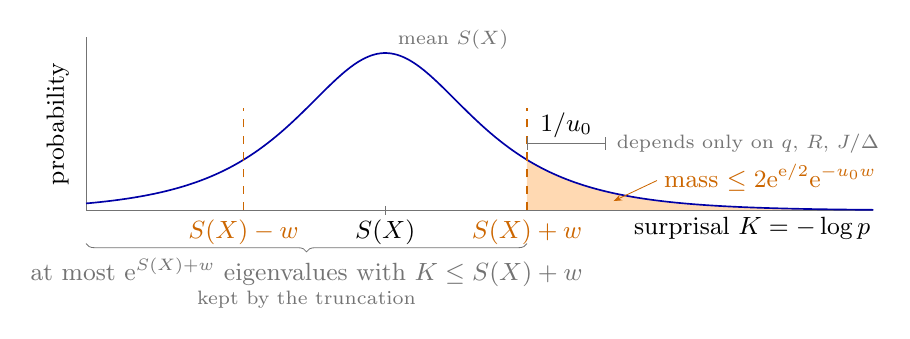
\begin{tikzpicture}[x=1cm, y=1cm, line width=0.3pt,
    lab/.style={font=\small, inner sep=1pt},
    name/.style={font=\scriptsize, text=black!55, inner sep=1pt},
    brace/.style={decorate, decoration={brace, mirror, amplitude=3pt}},
    cut/.style={dashed, color=orange!80!black, line width=0.5pt}]
  \def\S{3.4}\def\w{1.8}\def\decay{1}\def\xmax{9.6}\def\xmin{-0.4}
  \fill[orange!30] plot[domain=5.2:\xmax, samples=60, smooth]
    (\x, {2/cosh(\x-\S)}) -- (\xmax, 0) -- (5.2, 0) -- cycle;
  \draw[black!55] (\xmin, 0) -- (\xmax, 0);
  \draw[black!55] (\xmin, 0) -- (\xmin, 2.2);
  \node[lab, anchor=north east] at (\xmax, -0.05) {surprisal \(K=-\log p\)};
  \node[lab, anchor=south, rotate=90] at (\xmin-0.18, 1.1) {probability};
  \draw[blue!65!black, line width=0.6pt] plot[domain=\xmin:\xmax, samples=120, smooth]
    (\x, {2/cosh(\x-\S)});
  \node[name, anchor=south west] at (\S+0.12, 2.0) {mean \(S(X)\)};
  \draw[black!55] (\S, 0.06) -- (\S, -0.06);
  \node[lab, anchor=north] at (\S, -0.08) {\(S(X)\)};
  \draw[cut] (\S-\w, 0) -- (\S-\w, 1.3);
  \draw[cut] (\S+\w, 0) -- (\S+\w, 1.3);
  \node[lab, anchor=north, text=orange!80!black] at (\S-\w, -0.08) {\(S(X)-w\)};
  \node[lab, anchor=north, text=orange!80!black] at (\S+\w, -0.08) {\(S(X)+w\)};
  \draw[black!55, {Bar}-{Bar}, line width=0.4pt] (\S+\w, 0.85) -- (\S+\w+\decay, 0.85);
  \node[lab, anchor=south] at (\S+\w+0.5*\decay, 0.88) {\(1/u_0\)};
  \node[name, anchor=west] at (\S+\w+\decay+0.1, 0.85) {depends only on \(q\), \(R\), \(J/\Delta\)};
  \node[lab, anchor=west, text=orange!80!black] at (\S+\w+1.7, 0.42)
    {mass \(\le 2\mathrm{e}^{\mathrm{e}/2}\mathrm{e}^{-u_0w}\)};
  \draw[orange!80!black, -{Stealth[length=3pt]}] (\S+\w+1.65, 0.38) -- (\S+\w+1.1, 0.12);
  \draw[brace, black!55] (\xmin, -0.42) -- (\S+\w, -0.42)
    node[lab, midway, below=4pt] {at most \(\mathrm{e}^{S(X)+w}\) eigenvalues with \(K\le S(X)+w\)}
    node[name, midway, below=16pt] {kept by the truncation};
\end{tikzpicture}

\end{adjustbox}
\caption{Schematic law of the surprisal. The tails decay exponentially at rate $u_0$; the mass beyond $S(X)+w$ is at most $2e^{e/2}e^{-u_0w}$, and at most $e^{S(X)+w}$ eigenvalues lie to the left of that line. Both facts are reused for the sequential truncation in Part II.}\label{fig:tail-sketch}
\end{figure}

\begin{remark}[Rényi entropies near one]\label{rem:renyi}
For $0<u\le u_0$ and $\alpha=1-u$, \eqref{eq:mgf} reads
$S_\alpha(X)=\frac{1}{u}\log\Tr\rho_X^{\alpha}\le S(X)+512\e\vartheta\cB_R(1-\alpha)$.
Since $S_\alpha\ge S$ for $\alpha<1$, all Rényi entropies of order
$\alpha\in[1-u_0,1]$ of an interval lie within $16\e\sqrt{(1+\vartheta)\cB_R}$ of its von
Neumann entropy. This is used in Section~\ref{sec:shortcut}.
\end{remark}

\section{The buffered discount with a constant-width buffer}\label{sec:buffer}

\begin{inwords}
This section establishes the core variational estimate of Part~\ref{part:arealaw}.
Conditioning an interval $X$ on a buffer $T$ of a constant number of
nearby sites halves its entropy, up to an additive constant:
\[
 S(X\,|\,T)\ \le\ \tfrac12\,S(X)+C .
\]
To keep the excitation energy of the filtered vector below the gap
$\Delta$, the filtering is distributed across $m$ concentric shells
$X_j=X^{+jD}$ ($j=1,\dots,m$), each wider than the previous one by a step $D=R$, with flanking buffers
$T_j=X_j\setminus X$ and small per-shell weight $a_j=2/m$ summing to
$\sum_j a_j=2$. Choosing $m$ of order $1+J/\Delta$ keeps the total buffer
$T=T_m$ of \emph{constant} width $mD$ on each side of $X$.

Specifically, we apply to $\Om$ a product $K=L_m\cdots L_1$ of positive
operators $L_j$ acting on $X_j$, each normalised by $\Tr L_j^{2/a_j}=1$,
and maximise the norm $N=\norm{K\Om}$. Two complementary bounds on the
maximum $N$ yield the discount.

\emph{Upper bound on $N$ (lower bound on $-2\log N$).} Computing the
excitation energy of the normalised filtered vector $\phi=K\Om/N$ requires
controlling the conjugation of each Hamiltonian term by all $m$ filters.
At a maximiser of $N$, however, unitary stationarity implies that each
filter $L_j$ commutes with the reduced density operator $\rho_j$ of $\phi$
on its own shell $X_j$. This commutation gives a \emph{stripping
identity}: any operator supported inside $X_k$ is unchanged in expectation
when conjugated by the outer filter $L_k$. Because consecutive shells are
separated by $D\ge R$, any range-$R$ interaction $h_Y$ is split by at most
one shell $X_j$; all outer filters ($k>j$) contain $Y$ and strip away,
while all inner filters ($k<j$) are disjoint from $Y$ and commute past
$h_Y$. Thus $h_Y$ is conjugated by $L_j$ alone. Diagonal stationarity clips
the log-eigenvalue differences of $L_j$ to $a_j/2$ times those of $\rho_j$,
so conjugation by $L_j$ changes the expectation of $h_Y$ by at most
$O(Ja_j^2)$. Summing over the $m$ shells and the at most $N_R$ interactions
split by each shell bounds the excitation energy of $\phi$ by
$O(J\sum_j a_j^2)=O(J/m)$. The spectral gap then ensures a ground-state
overlap $\abs{\langle\Om,\phi\rangle}^2\ge 1-C/(m\Delta)$, and the same
holds for every prefix optimiser. Using this overlap to peel the filters
$L_j$ off one at a time, and bounding each peeled factor by
$\norm{L_j\Om}\le\exp(-a_jS(X_j)/2+Ca_j^2)$ via Schatten--Hölder and the
marginal tail bound (Lemma~\ref{lem:tail}), gives
$-2\log N\ge\sum_ja_jS(X_j)-C$.

\emph{Lower bound on $N$ (upper bound on $-2\log N$).} Conversely, we test
the variational maximum on trial filters that ``pin'' a single Schmidt
vector $u_i$ of $\Om=\sum_i\sqrt{p_i}\,u_i\otimes w_i$ across $X$: namely
$L_j=\ket{u_i}\bra{u_i}\otimes M_j$, where $M_j$ acts only on the flank
$T_j$. This decouples $X$ and produces $\sqrt{p_i}\,u_i$ tensored with
$M_m\cdots M_1w_i$. Because the flank filters $M_j$ act on nested sets and
need not commute, we relate the norm of their product to the sum of single-flank
entropies via three-lines interpolation on $M_m^z\cdots M_1^zw_i$, finding
that $M_j$ can be chosen so that
$\norm{M_m\cdots M_1w_i}\ge\exp(-\sum_ja_jS_{w_i}(T_j)/2)$. Averaging over
$i$ with weights $p_i$ and applying concavity of the entropy gives
$-2\log N\le S(X)+\sum_ja_jS(T_j)$.

Subtracting the two bounds yields $\sum_ja_j\,[S(X_j)-S(T_j)]\le S(X)+C$.
Here $S(X_j)-S(T_j)=S(X|T_j)$, which is monotone decreasing in $j$ by
strong subadditivity. Since $\sum_ja_j=2$, the discount follows. No
property of the state on the flanks is used beyond their containing a
constant number of sites, and no spectral gap of any restricted
Hamiltonian is invoked.
\end{inwords}

\precisely
Fix $D=R$ (recall $R\ge1$) and an integer $m\ge4$. For an interval $X\subseteq\Lam$
put
\[
\begin{split}
 &X_0=X,\qquad X_j=X^{+jD}\ (1\le j\le m),\\
 &T_j=X_j\setminus X,
 \qquad a_j=\frac2m .
\end{split}
\]
Then $T_1\subseteq\cdots\subseteq T_m$, each $T_j$ consists of at most two
intervals of length at most $jD$, and $\sum_ja_j=2$. Define the constants
\begin{equation}\label{eq:CE}
\begin{split}
 &C_E:=8\,N_R\,J\,q^{2(R+1)},\\
 &m:=\Bigl\lceil\max\Bigl\{4,\ \frac{4C_E}{\Delta},\ 128\sqrt{(1+\vartheta)\cB_R},\\
 &\qquad\qquad\qquad
 4096\,\e\,(1+\vartheta)\,\cB_R\Bigr\}\Bigr\rceil .
\end{split}
\end{equation}
Every entry in the maximum is bounded by a function of $q,R$ times
$(1+J/\Delta)$, so
\begin{equation}\label{eq:mbound}
 m\le C_1(q,R)\,(1+\vartheta).
\end{equation}

\begin{figure*}[t]
\centering
\begin{adjustbox}{max width=\linewidth}
\begin{tenkz}[lattice={1x14}, frame=plane, physical=up, bonds=none]
  \tn{} & \tn{} & \tn{} & \tn{} & \tn{} & \tn{} & \tn{} & \tn{} & \tn{} & \tn{} & \tn{} & \tn{} & \tn{} & \tn{}
  \tnmark[form=enclosure, species=selected, label pos=s]{(1,6) .. (1,8)}{$X$}
  \tnmark[form=enclosure, species=secondary, label pos=n]{(1,4) .. (1,10)}{$X_1=X^{+D}$}
  \tnmark[form=enclosure, species=collar, label pos=150]{(1,2) .. (1,12)}{$X_2=X^{+2D}$}
  \tnmark[form=bracket, species=complement, label pos=s]{(1,4) .. (1,5)}{$T_1$}
  \tnmark[form=bracket, species=complement, label pos=s]{(1,9) .. (1,10)}{$T_1$}
  \tnmark[form=bracket, species=complement, label pos=s]{(1,2) .. (1,5)}{$T_2$}
  \tnmark[form=bracket, species=complement, label pos=s]{(1,9) .. (1,12)}{$T_2$}
\end{tenkz}

\end{adjustbox}
\caption{The interval $X$ and the nested shells $X_1=X^{+D}\subset X_2=X^{+2D}$, drawn with $D=R=2$; the braces mark the flanks $T_j=X_j\setminus X$, each a union of at most two intervals of length at most $jD$, which carry the buffer.}\label{fig:chain-shells}
\end{figure*}

\begin{lemma}[Single splitting]\label{lem:singlesplit}
A support $Y$ with $\diam_{d_\Lam}Y\le R$ is split by at most one of the
intervals $X_1,\dots,X_m$. If it is split by $X_j$, it is contained in
$X_i$ for every $i>j$ and disjoint from $X_i$ for every $i<j$. The same
holds verbatim for the family $X_0,\dots,X_m$.
\end{lemma}
\begin{proof}
Suppose $Y$ is split by $X_j$. Then $Y$ contains a site $y\notin X_j$ and
a site $x\in X_j$, and all sites of $Y$ lie within graph distance $R\le D$
of both $x$ and $y$. Every site within distance $D$ of $X_j$ belongs to
$X_{j+1}$, so $Y\subseteq X_{j+1}\subseteq X_i$ for all $i>j$. Conversely,
every site of $X_{j-1}$ lies at distance greater than $D$ from $\Lam\setminus X_j$
(since $X_j=X_{j-1}^{+D}$), so $Y\cap X_{j-1}=\varnothing$, and hence
$Y\cap X_i=\varnothing$ for all $i<j$. A set that is contained in $X_i$ or
disjoint from $X_i$ is not split by $X_i$.
\end{proof}

\begin{lemma}[Buffered discount]\label{lem:buffer}
With $m$ as in \eqref{eq:CE}, every interval $X\subseteq\Lam$ satisfies
\begin{equation}\label{eq:discount}
 S(X\,|\,T_m)\ \le\ \frac12\,S(X)+\frac12+\frac{C_E}{\Delta}.
\end{equation}
\end{lemma}

\begin{proof}
If $X=\varnothing$ both sides vanish. Assume $X\ne\varnothing$.

\paragraph{The optimisation.}
To ensure that the feasible sets are nonempty and every filter is invertible,
fix $\epsilon>0$ so small that $(\dim\cH_{X_j})\epsilon^{2/a_j}<1$ for all
$j$, and maximise
\[
 N=\norm{L_m\cdots L_1\Om}
\]
over positive operators $L_j$ on $\cH_{X_j}$ (extended by the identity on
$\Lam\setminus X_j$) satisfying $L_j\ge\epsilon\id$ and
$\Tr_{\cH_{X_j}}L_j^{2/a_j}=1$. The feasible sets are nonempty and compact
and every feasible product is invertible, so a maximum $N>0$ is attained.
At a maximiser put $K=L_m\cdots L_1$, $\phi=K\Om/N$, and
$\rho_j=\Tr_{\Lam\setminus X_j}\ket\phi\bra\phi$.

\begin{figure*}[t]
\centering
\begin{adjustbox}{max width=\linewidth}
\(\displaystyle N=\Biggl\|
  \begin{tenkz}[rows={wire,wire,wire,wire}, cols=7, bonds=none]
    \tn[at=(4,1), skin=box, wide=7, name=o,
        ports={90@1:physical, 90@2:physical, 90@3:physical, 90@4:physical,
               90@5:physical, 90@6:physical, 90@7:physical}]{\Omega}
    \tn[at=(3,3), skin=box, wide=3, name=l1,
        ports={270@1:physical, 270@2:physical, 270@3:physical,
               90@1:physical, 90@2:physical, 90@3:physical}]{L_1}
    \tn[at=(2,2), skin=box, wide=5, name=l2,
        ports={270@1:physical, 270@2:physical, 270@3:physical, 270@4:physical, 270@5:physical,
               90@1:physical, 90@2:physical, 90@3:physical, 90@4:physical, 90@5:physical}]{L_2}
    \tn[at=(1,1), skin=box, wide=7, name=l3,
        ports={270@1:physical, 270@2:physical, 270@3:physical, 270@4:physical,
               270@5:physical, 270@6:physical, 270@7:physical,
               90@1:physical:$T_3$, 90@2:physical, 90@3:physical, 90@4:physical:$X$,
               90@5:physical, 90@6:physical, 90@7:physical:$T_3$}]{L_3}
    \tnwire{o.90@3}{l1.270@1} \tnwire{o.90@4}{l1.270@2} \tnwire{o.90@5}{l1.270@3}
    \tnwire{l1.90@1}{l2.270@2} \tnwire{l1.90@2}{l2.270@3} \tnwire{l1.90@3}{l2.270@4}
    \tnwire{o.90@2}{l2.270@1} \tnwire{o.90@6}{l2.270@5}
    \tnwire{l2.90@1}{l3.270@2} \tnwire{l2.90@2}{l3.270@3} \tnwire{l2.90@3}{l3.270@4}
    \tnwire{l2.90@4}{l3.270@5} \tnwire{l2.90@5}{l3.270@6}
    \tnwire{o.90@1}{l3.270@1} \tnwire{o.90@7}{l3.270@7}
  \end{tenkz}
  \Biggr\|\)

\end{adjustbox}
\caption{The optimized norm. Three positive filters $L_1,L_2,L_3$ act on the nested intervals $X_1\subset X_2\subset X_3$ of the ground vector; each is normalized by $\mathrm{Tr}\,L_j^{2/a_j}=1$.}\label{fig:filter-product}
\end{figure*}

\paragraph{Stationarity.}
To eliminate outer filters when evaluating expectations of operators
supported in inner shells, we prove that $[L_j,\rho_j]=0$ for all $j$ by
descending induction on $j$. The key mechanism is the stripping identity:
if $[L_k,\rho_k]=0$ and $T$ is supported in $X_k$, then
\begin{equation}\label{eq:strip}
 \langle\phi,L_kTL_k^{-1}\phi\rangle=\Tr(L_k^{-1}\rho_kL_kT)=\Tr(\rho_kT)=\langle\phi,T\phi\rangle .
\end{equation}
Assume $[L_k,\rho_k]=0$ for all $k>j$ and let $B$ be anti-Hermitian on
$\cH_{X_j}$. Replacing $L_j$ by $\e^{tB}L_j\e^{-tB}$ preserves both
constraints, so the derivative of $\log\norm{K\Om}$ at $t=0$ vanishes.
That derivative equals
$\Re\langle\phi,K_{>j}(B-L_jBL_j^{-1})K_{>j}^{-1}\phi\rangle$ with
$K_{>j}=L_m\cdots L_{j+1}$. Because $B-L_jBL_j^{-1}$ is supported in
$X_j\subseteq X_{j+1}\subseteq\cdots\subseteq X_m$, we can strip $L_m$ by
\eqref{eq:strip}, then $L_{m-1}$, and so on down to $L_{j+1}$. Since
$\Tr(\rho_jB)$ is purely imaginary, stationarity yields
$\Re\Tr(L_j^{-1}\rho_jL_jB)=0$ for all anti-Hermitian $B$. Hence
$L_j^{-1}\rho_jL_j$ is Hermitian, i.e.\ equal to $L_j\rho_jL_j^{-1}$, so
$\rho_j$ commutes with $L_j^2$ and therefore with $L_j\ge0$. No
commutation between distinct filters is claimed or used.

To bound the eigenvalue ratios of $L_j$ in terms of those of $\rho_j$,
choose a common eigenbasis of $L_j$ and $\rho_j$ with eigenvalues $l_i$
and $p_i$, and set $x_i=l_i^{2/a_j}$, so that $\sum_ix_i=1$ and
$x_i\ge\epsilon^{2/a_j}$. A diagonal variation of $L_j$ together with the
same stripping of $K_{>j}$ gives
$d\log N=\frac{a_j}2\sum_ip_i\,dx_i/x_i$. By the Kuhn--Tucker conditions
on the simplex with floor $\epsilon^{2/a_j}$, the ratio $p_i/x_i$ equals a
constant $\lambda>0$ on all coordinates above the floor and is at most
$\lambda$ on floored coordinates (at least one coordinate lies strictly
above the floor by the choice of $\epsilon$, and $\lambda>0$ because
shifting weight from a zero-probability free coordinate to a
positive-probability floored coordinate would strictly increase $N$). Thus
$x_i=\max\{\epsilon^{2/a_j},p_i/\lambda\}$. Because taking a maximum with
a common floor contracts differences of logarithms, we obtain
\begin{equation}\label{eq:clip}
 \Bigl|\log\frac{l_i}{l_k}\Bigr|\le\frac{a_j}{2}\Bigl|\log\frac{p_i}{p_k}\Bigr|
 \qquad(p_i,p_k>0).
\end{equation}

\paragraph{Energy of the optimised vector.}
Since $KHK^{-1}\phi=E_0\phi$, the excitation energy of $\phi$ is
\[
 \langle\phi,(H-E_0)\phi\rangle=\sum_Y\Re\bigl(\langle\phi,h_Y\phi\rangle-\langle\phi,Kh_YK^{-1}\phi\rangle\bigr).
\]
If $Y$ is split by none of $X_1,\dots,X_m$, then by
Lemma~\ref{lem:singlesplit} each $X_j$ either contains $Y$ or is disjoint
from $Y$; stripping the containing filters from the outside in via
\eqref{eq:strip} and commuting the disjoint filters past $h_Y$ shows that
the summand vanishes. If $Y$ is split by $X_j$, the same reduction strips
$L_m,\dots,L_{j+1}$ and commutes $L_{j-1},\dots,L_1$ past $h_Y$, leaving
only the single-filter difference
$\langle\phi,h_Y\phi\rangle-\langle\phi,L_jh_YL_j^{-1}\phi\rangle$. Write
$\phi=\sum_i\sqrt{p_i}\,e_i\otimes f_i$ for the Schmidt decomposition of
$\phi$ across $X_j$, where the $e_i$ are chosen in a common eigenbasis of
$\rho_j$ and $L_j$ (diagonalising $L_j$ within each eigenspace of
$\rho_j$), and put
$h_{ik}=\langle e_i\otimes f_i,h_Y(e_k\otimes f_k)\rangle$. Pairing
$(i,k)$ with $(k,i)$ and using $h_{ki}=\overline{h_{ik}}$ gives
\[
\begin{split}
 &\Re\langle\phi,L_jh_YL_j^{-1}\phi\rangle-\langle\phi,h_Y\phi\rangle\\
 &\qquad=\sum_{i,k:\,p_ip_k>0}\sqrt{p_ip_k}\,\bigl(\cosh(\log(l_i/l_k))-1\bigr)\Re h_{ik}.
\end{split}
\]
Set $z=\frac12\log(p_i/p_k)$. By \eqref{eq:clip} and $a_j\le\frac12$, we
have
$\cosh(\log(l_i/l_k))-1\le\cosh(a_jz)-1\le\frac12a_j^2z^2\cosh(a_jz)\le\frac12a_j^2z^2\cosh(z/2)$,
while $\sqrt{p_ip_k}=(p_i+p_k)/(2\cosh z)$. Since
$\sup_z z^2\cosh(z/2)/(4\cosh z)\le1$, the prefactor of $\Re h_{ik}$ is at
most $a_j^2(p_i+p_k)$. Expanding $h_Y$ in matrix units via
\eqref{eq:matrixunits} and applying \eqref{eq:rowcolumn} to each product
term yields
\[
 \bigl|\Re\langle\phi,L_jh_YL_j^{-1}\phi\rangle-\langle\phi,h_Y\phi\rangle\bigr|
 \le 2a_j^2\,q^{2(R+1)}J .
\]
Summing over $j=1,\dots,m$ and the at most $N_R$ interactions split by
each $X_j$ gives
\begin{equation}\label{eq:energy}
\begin{split}
 &0\le\langle\phi,(H-E_0)\phi\rangle\le\sum_{j=1}^m N_R\cdot 2a_j^2q^{2(R+1)}J\\
 &\qquad=\frac{8N_RJq^{2(R+1)}}{m}=\frac{C_E}{m}.
\end{split}
\end{equation}
By the spectral gap \eqref{eq:gap} and the definition of $m$ in \eqref{eq:CE},
\begin{equation}\label{eq:overlap}
 1-\abs{\langle\Om,\phi\rangle}^2\le\frac{C_E}{m\Delta}\le\frac14 .
\end{equation}
The exact same bound holds for the optimiser of every prefix
$L_j\cdots L_1$ ($1\le j\le m$): the stationarity and energy arguments
apply verbatim to the $j$-shell problem with the same weights and floor,
and any interaction split by $X_k$ with $k>j$ is disjoint from
$X_1,\dots,X_j$ and contributes zero, so the prefix excitation energy is
bounded by the sum in \eqref{eq:energy} truncated to $i\le j$.

\begin{figure*}[t]
\centering
\begin{adjustbox}{max width=\linewidth}
\(\displaystyle \begin{gathered}
    \langle\phi,Kh_YK^{-1}\phi\rangle
    \;=\;
    \Bigl\langle\phi,\;
    \begin{quantikz}
      \lstick{$X_{j-1}$} & \gate[2]{L_j^{-1}} & & \gate[2]{L_j} & \\
      \lstick{$X_j\setminus X_{j-1}$} & & \gate[2]{h_Y} & & \\
      \lstick{$\Lambda\setminus X_j$} & & & &
    \end{quantikz}
    \;\phi\Bigr\rangle
    \\[2pt]
    \text{\small outer filters $L_{j+1},\dots,L_m$: stripped by the stripping identity, $[L_k,\rho_k]=0$}
    \\[-1pt]
    \text{\small inner filters $L_1,\dots,L_{j-1}$: disjoint from $Y$, commute with $h_Y$}
  \end{gathered}\)

\end{adjustbox}
\caption{Why the energy is small. An interaction $h_Y$ split by $X_j$ is conjugated by exactly one filter: the outer filters, whose regions contain $Y$, are stripped by the stripping identity at the optimum, and the inner ones commute with $h_Y$ because they live on disjoint sites.}\label{fig:qc-single-split}
\end{figure*}

\paragraph{Upper bound on the optimum.}
To peel the filters off one by one, let $N_j$ be the maximum norm for the
prefix $1,\dots,j$ at the same floor $\epsilon$ (with $N_0=1$), and let
$L_j\cdots L_1$ be a prefix-$j$ maximiser with $K_{<j}=L_{j-1}\cdots L_1$.
Applying \eqref{eq:overlap} to the prefix-$j$ maximiser and using
Cauchy--Schwarz gives
\[
\begin{split}
 &\sqrt{1-C_E/(m\Delta)}\;N_j\le\abs{\langle\Om,L_jK_{<j}\Om\rangle}\\
 &\qquad=\abs{\langle L_j\Om,K_{<j}\Om\rangle}\le\norm{L_j\Om}\,N_{j-1}.
\end{split}
\]
For any feasible $L_j$, Schatten--Hölder with conjugate exponents
$\frac1{1-a_j}$ and $\frac1{a_j}$ together with $\Tr L_j^{2/a_j}=1$ gives
\[
 \norm{L_j\Om}^2=\Tr\rho_{X_j}L_j^2\le\bigl(\Tr\rho_{X_j}^{1/(1-a_j)}\bigr)^{1-a_j}.
\]
Applying Lemma~\ref{lem:tail} to the interval $X_j$ at
$u=-a_j/(1-a_j)$ (which satisfies $\abs u\le 2a_j=4/m\le u_0$ by
\eqref{eq:CE}) and using $(1-a_j)u^2\le 2a_j^2$ yields
\[
 \log\norm{L_j\Om}^2\le -a_jS(X_j)+1024\,\e\,\vartheta\,\cB_R\,a_j^2 .
\]
Multiplying the recursion $N_j\le(1-C_E/(m\Delta))^{-1/2}\norm{L_j\Om}N_{j-1}$
over $j=1,\dots,m$ and using $-\frac12\log(1-v)\le v$ for $0\le v\le\frac12$,
we obtain
\[
\begin{split}
 &\log N\le-\frac12\sum_ja_jS(X_j)+512\,\e\,\vartheta\,\cB_R\sum_ja_j^2+\frac{mC_E}{m\Delta}\\
 &\qquad\le -\frac12\sum_ja_jS(X_j)+\frac12+\frac{C_E}{\Delta},
\end{split}
\]
since $\sum_ja_j^2=4/m\le 1/(1024\e\vartheta\cB_R)$ by \eqref{eq:CE}. Equivalently,
\begin{equation}\label{eq:lowerN}
 -2\log N\ \ge\ \sum_{j=1}^ma_jS(X_j)-1-\frac{2C_E}{\Delta},
\end{equation}
with constants independent of the floor $\epsilon$.

\paragraph{Lower bound on the optimum by Schmidt pinning.}
Letting $\epsilon\downarrow0$, the floored maxima converge to the supremum
$N$ over all nonnegative filters $L_j\ge0$ satisfying $\Tr L_j^{2/a_j}=1$
(since the feasible sets are compact and every nonnegative feasible filter
is a limit of strictly positive feasible ones), and \eqref{eq:lowerN}
continues to hold. Write $\Om=\sum_i\sqrt{p_i}\,u_i\otimes w_i$ ($p_i>0$)
for the Schmidt decomposition across $X$. For each fixed $i$, test $N$ on
the trial filters
\[
\begin{split}
 &L_j=\ket{u_i}\bra{u_i}\otimes M_j,\qquad M_j\ge0\text{ on }\cH_{T_j},\\
 &\Tr M_j^{2/a_j}=1,
\end{split}
\]
which are feasible (since $\Tr_{X_j}L_j^{2/a_j}=\Tr M_j^{2/a_j}=1$) and give
$N\ge\sqrt{p_i}\,N_i$, where $N_i=\sup\norm{M_m\cdots M_1w_i}$ over such $M_j$.
We claim that
\begin{equation}\label{eq:trial}
 \log N_i\ge-\frac12\sum_ja_jS_{w_i}(T_j).
\end{equation}
Because the flank filters $M_1,\dots,M_m$ act on nested regions
$T_1\subseteq\cdots\subseteq T_m$ and need not commute, we relate the
product norm $N_i$ to single-flank expectations by complex interpolation.
Fix invertible feasible $M_j$ and consider the analytic vector-valued
function $F_i(z)=M_m^z\cdots M_1^zw_i$ on the strip $0\le\Re z\le1$. On
$\Re z=0$, the factors $M_j^{iy}$ are unitary and $\norm{F_i(iy)}=1$. On
$\Re z=1$, set $U_j=M_j^{iy}$, $V_j=U_j\cdots U_1$, and $V_0=\id$;
collecting the unitaries to the left gives
\[
\begin{split}
 &M_m^{1+iy}\cdots M_1^{1+iy}\\
 &\qquad=(U_m\cdots U_1)\,(V_{m-1}^*M_mV_{m-1})\cdots(V_0^*M_1V_0).
\end{split}
\]
Each conjugated factor $V_{j-1}^*M_jV_{j-1}$ is positive, supported in
$T_j$ (since $V_{j-1}$ acts on $T_{j-1}\subseteq T_j$), and satisfies the
same trace-power normalisation, so $\norm{F_i(1+iy)}\le N_i$. Testing
$F_i(z)$ against arbitrary unit vectors and applying Hadamard's
three-lines theorem yields $\log\norm{F_i(x)}\le x\log N_i$ for
$0\le x\le1$; differentiating at $x=0^+$ gives
$\sum_j\langle w_i,\log M_j\,w_i\rangle\le\log N_i$. Choosing
$M_j=\bigl((1-\delta)\rho_{w_i,T_j}+\delta\id/\dim\cH_{T_j}\bigr)^{a_j/2}$ and
letting $\delta\downarrow0$, the left-hand side converges to
$-\frac12\sum_ja_jS_{w_i}(T_j)$, proving \eqref{eq:trial}. Consequently,
$-2\log N\le-\log p_i+\sum_ja_jS_{w_i}(T_j)$ for every $i$. Averaging over
$i$ with weights $p_i$ and using concavity of the entropy (since
$\sum_ip_i\rho_{w_i,T_j}=\rho_{T_j}$) gives
\begin{equation}\label{eq:upperN}
 -2\log N\le S(X)+\sum_{j=1}^ma_jS(T_j).
\end{equation}

\begin{figure*}[t]
\centering
\begin{adjustbox}{max width=\linewidth}
\(\displaystyle \begin{aligned}
  &\begin{tenkz}[rows={wire}, cols=6, bonds=none]
    \tn[at=(1,1), skin=box, wide=6, name=o,
        ports={90@1:physical:$X$, 90@3:physical:$T_1$,
               90@4:physical:$T_2\setminus T_1$, 90@6:physical:$\Lambda\setminus X_2$}]{\Omega}
  \end{tenkz}
  \;=\;\sum_i\sqrt{p_i}\;\;
  \begin{tenkz}[rows={wire}, cols=6, bonds=none]
    \tn[at=(1,1), skin=box, name=u, ports={90:physical:$X$}]{u_i}
    \tn[at=(1,3), skin=box, wide=4, name=w,
        ports={90@1:physical:$T_1$, 90@2:physical:$T_2\setminus T_1$,
               90@4:physical:$\Lambda\setminus X_2$}]{w_i}
  \end{tenkz}
  \\[2ex]
  &\begin{tenkz}[rows={wire,wire,wire}, cols=6, bonds=none]
    \tn[at=(3,1), skin=box, wide=6, name=o,
        ports={90@1:physical, 90@3:physical, 90@4:physical, 90@6:physical}]{\Omega}
    \tn[at=(1,6), skin=none, name=ox, ports={270:physical, 90:physical:$\Lambda\setminus X_2$}]{}
    \tnwire{o.90@6}{ox.270}
    \tn[at=(1,1), skin=box, wide=2, name=p,
        ports={270@1:physical, 90@1:physical:$X$}]{\lvert u_i\rangle\langle u_i\rvert}
    \tn[at=(2,3), skin=box, name=m1,
        ports={270:physical, 90:physical}]{M_1}
    \tn[at=(1,3), skin=box, wide=2, name=m2,
        ports={270@1:physical, 270@2:physical,
               90@1:physical:$T_1$, 90@2:physical:$T_2\setminus T_1$}]{M_2}
    \tnwire{o.90@1}{p.270@1}
    \tnwire{o.90@3}{m1.270} \tnwire{m1.90}{m2.270@1}
    \tnwire{o.90@4}{m2.270@2}
  \end{tenkz}
  \;=\;\sqrt{p_i}\;\;
  \begin{tenkz}[rows={wire,wire,wire}, cols=6, bonds=none]
    \tn[at=(3,1), skin=box, name=u, ports={90:physical}]{u_i}
    \tn[at=(1,1), skin=none, name=ux, ports={270:physical, 90:physical:$X$}]{}
    \tnwire{u.90}{ux.270}
    \tn[at=(3,3), skin=box, wide=4, name=w,
        ports={90@1:physical, 90@2:physical, 90@4:physical}]{w_i}
    \tn[at=(1,6), skin=none, name=wx, ports={270:physical, 90:physical:$\Lambda\setminus X_2$}]{}
    \tnwire{w.90@4}{wx.270}
    \tn[at=(2,3), skin=box, name=m1,
        ports={270:physical, 90:physical}]{M_1}
    \tn[at=(1,3), skin=box, wide=2, name=m2,
        ports={270@1:physical, 270@2:physical,
               90@1:physical:$T_1$, 90@2:physical:$T_2\setminus T_1$}]{M_2}
    \tnwire{w.90@1}{m1.270} \tnwire{m1.90}{m2.270@1}
    \tnwire{w.90@2}{m2.270@2}
  \end{tenkz}
\end{aligned}\)

\end{adjustbox}
\caption{Schmidt pinning. With the trial filters $|u_i\rangle\langle u_i|\otimes M_j$ (the projector is drawn once, by idempotence; the flanks are grouped into one leg each), the filtered vector becomes $\sqrt{p_i}\,u_i$ tensored with the flank filters applied to the partner $w_i$, which lower-bounds the optimum by $-S(X)-\sum_ja_jS(T_j)$ in the exponent after averaging over $i$.}\label{fig:pinning}
\end{figure*}

\paragraph{Conclusion.}
Subtracting \eqref{eq:upperN} from \eqref{eq:lowerN} gives
$\sum_ja_j\bigl(S(X_j)-S(T_j)\bigr)\le S(X)+1+2C_E/\Delta$. Since
$S(X_j)-S(T_j)=S(XT_j)-S(T_j)=S(X|T_j)$ and $S(X|T_j)\ge S(X|T_m)$ for all
$j\le m$ by strong subadditivity (conditioning on the larger flank
$T_m\supseteq T_j$ can only decrease conditional entropy), $\sum_ja_j=2$
yields $2S(X|T_m)\le S(X)+1+2C_E/\Delta$.
\end{proof}

\section{Closing the argument}\label{sec:closing}

\begin{inwords}
Lemma~\ref{lem:buffer} shows that $S(X|T)\le\frac12S(X)+C$, where $T$ is a
buffer of a constant number of sites. On the other hand, conditional
entropy cannot be arbitrarily negative: by the Araki--Lieb triangle
inequality $S(XT)\ge S(X)-S(T)$, we have $S(X|T)\ge S(X)-2S(T)$. Combining
the two inequalities gives $S(X)-2S(T)\le\frac12S(X)+C$, hence
$S(X)\le 4S(T)+2C$. Since $S(T)$ is bounded by the number of sites of $T$
times $\log q$, the area law follows immediately.

Nothing further is needed on a line. In two dimensions, the same pair of
inequalities for a square $X$ of side $r$ and a buffer $T$ of width
proportional to $r$ gives $S(X)\le 4S(T)+Cr$; there $T$ is an annulus of
area $\sim r^2$ whose entropy is as unknown as that of $X$, so the
estimate does not close. That geometric obstruction is the exact reason
the two-dimensional proof requires the multi-scale machinery of \cite{AL}.
\end{inwords}

\precisely
\begin{proof}[Proof of Theorem~\ref{thm:A}]
By Lemma~\ref{lem:reductions} it suffices to bound $S(X)$ for an interval
$X$ in an interval domain. Let $T=T_m$ be the buffer of
Lemma~\ref{lem:buffer}, which contains at most $2mD$ sites. The Araki--Lieb
inequality $S(XT)\ge S(X)-S(T)$ gives $S(X|T)\ge S(X)-2S(T)$, and
\eqref{eq:discount} gives $S(X|T)\le\frac12S(X)+\frac12+C_E/\Delta$. Hence
\begin{equation}\label{eq:final}
 S(X)\le 4S(T)+1+\frac{2C_E}{\Delta}\le 8mD\log q+1+\frac{2C_E}{\Delta}=:C_{\mathrm{int}}.
\end{equation}
By \eqref{eq:mbound} and \eqref{eq:CE}, $C_{\mathrm{int}}\le C_0(q,R)(1+J/\Delta)$
with, for instance,
$C_0(q,R)=8C_1(q,R)\,R\log q+1+16N_Rq^{2(R+1)}$.
\end{proof}

\begin{figure*}[t]
\centering
\begin{adjustbox}{max width=\linewidth}
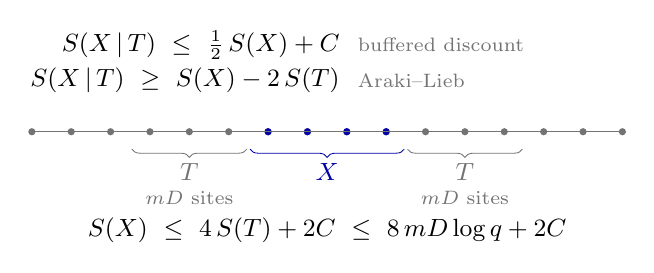
\begin{tikzpicture}[x=1cm, y=1cm, line width=0.3pt,
    site/.style={circle, fill=black!55, inner sep=0pt, minimum size=2.6pt},
    xsite/.style={site, fill=blue!65!black},
    brace/.style={decorate, decoration={brace, mirror, amplitude=3pt}},
    lab/.style={font=\small, inner sep=1pt},
    name/.style={font=\scriptsize, text=black!55, inner sep=1pt}]
  \foreach \i in {1,...,16} {
    \pgfmathsetmacro{\xx}{0.5*(\i-1)}
    \node[site] at (\xx, 0) {};
  }
  \foreach \i in {7,...,10} {
    \pgfmathsetmacro{\xx}{0.5*(\i-1)}
    \node[xsite] at (\xx, 0) {};
  }
  \draw[black!55] (0,0) -- (7.5,0);
  \draw[brace, blue!65!black] (2.77,-0.22) -- (4.73,-0.22)
    node[lab, midway, below=4pt, text=blue!65!black] {\(X\)};
  \draw[brace, black!55] (1.27,-0.22) -- (2.73,-0.22)
    node[lab, midway, below=4pt] {\(T\)}
    node[name, midway, below=14pt] {\(mD\) sites};
  \draw[brace, black!55] (4.77,-0.22) -- (6.23,-0.22)
    node[lab, midway, below=4pt] {\(T\)}
    node[name, midway, below=14pt] {\(mD\) sites};
  \node[lab, anchor=east] at (3.95, 1.1) {\(S(X\,|\,T)\ \le\ \tfrac12\,S(X)+C\)};
  \node[name, anchor=west] at (4.1, 1.1) {buffered discount};
  \node[lab, anchor=east] at (3.95, 0.65) {\(S(X\,|\,T)\ \ge\ S(X)-2\,S(T)\)};
  \node[name, anchor=west] at (4.1, 0.65) {Araki--Lieb};
  \node[lab, anchor=north] at (3.75, -1.05) {\(S(X)\ \le\ 4\,S(T)+2C\ \le\ 8\,mD\log q+2C\)};
\end{tikzpicture}

\end{adjustbox}
\caption{The closing step. The interval $X$ with its constant-width buffers $T$; the discount bounds $S(X|T)$ from above, Araki–Lieb from below, and $T$ has at most $2mD$ sites.}\label{fig:closing}
\end{figure*}

\begin{remark}[What the constant depends on]\label{rem:constants}
The spectral gap enters only through $\vartheta=J/\Delta$, linearly. The
dependence on the local dimension and interaction range enters through
$N_R\,q^{2(R+1)}$, which for nearest-neighbour interactions ($R=1$) is of
order $q^4$. The constants in Section~\ref{sec:buffer} were chosen for
simplicity rather than sharpness; Remark~\ref{rem:sharper} shows that the
polynomial dependence on $q$ is an artifact of bounding the matrix-unit
expansion term by term. By comparison, the bound of
Arad--Kitaev--Landau--Vazirani \cite{AKLV} is $\tilde O(\log^3(q)/\Delta)$
for $R=1$.
\end{remark}

\begin{remark}[Sharper constants, and what is intrinsic]\label{rem:sharper}
Three aspects of the constants in \eqref{eq:final} are not intrinsic to
the argument.

\emph{The count $N_R$.} The bound $2\cdot2^{2R}$ allows a separate
interaction term for every subset of a $2R$-site window. When the
Hamiltonian has one term per window of $R+1$ consecutive sites, a cut edge
splits at most $R$ of them, so $N_R$ may be replaced by $2R$.

\emph{The factor $q^{2(R+1)}$ in $C_E$.} This factor enters
\eqref{eq:energy} because the matrix-unit expansion \eqref{eq:matrixunits}
was bounded term by term. In the proof of Lemma~\ref{lem:tail}, the same
dimensional factor was converted into a logarithm via Hadamard's
three-lines theorem, and the identical device applies here. For a split
term $h=h_Y$ and the optimal filter $L=L_j$, define the entire function
$g(z)=\langle\phi,L^zhL^{-z}\phi\rangle$. Then
$g(0)=\langle\phi,h\phi\rangle$, $g(1)=\langle\phi,LhL^{-1}\phi\rangle$,
$\abs{g(iy)}\le J$ because $L^{iy}$ is unitary, and
$g(-\bar z)=\overline{g(z)}$. In the common eigenbasis of $\rho_j$ and $L_j$,
$g(z)=\sum_{i,k}\sqrt{p_ip_k}\,(l_i/l_k)^zh_{ik}$, and \eqref{eq:clip}
together with the weighted arithmetic--geometric mean inequality gives
$\sqrt{p_ip_k}\,\abs{(l_i/l_k)^z}\le p_i+p_k$ for $\abs{\Re z}\le1/a_j$;
hence $\abs{g(z)}\le 2Jq^{2(R+1)}$ on that strip by \eqref{eq:rowcolumn}.
Since $\log(2q^{2(R+1)})\le2\ell_R$, the three-lines theorem gives
$\abs{g(z)}\le\e J$ for $\abs{\Re z}\le 1/(2a_j\ell_R)$, and Cauchy's
estimate as in \eqref{eq:quadratic} yields, because $a_j\le1/(4\ell_R)$,
\[
 \abs{\Re\bigl(g(1)-g(0)\bigr)}\le 8\,\e\,J\,\ell_R^2\,a_j^2 .
\]
Thus \eqref{eq:energy} holds with $2a_j^2q^{2(R+1)}J$ replaced by
$8\e J\ell_R^2a_j^2$, i.e.\ with
\[
 C_E'=32\,\e\,N_R\,J\,\ell_R^2\le 32\,\e\,J\,\cB_R
\]
in place of $C_E$. The entry $4C_E'/\Delta$ in \eqref{eq:CE} is then
dominated by $4096\e(1+\vartheta)\cB_R$, and \eqref{eq:final} becomes
\[
 S(X)\ \le\ C\,(1+J/\Delta)\,\cB_R\,R\log q,
\]
where now $\cB_R\le 1+2R\bigl(1+(R+1)\log q\bigr)^2$ and $C$ is an absolute
constant.
For nearest-neighbour chains this is
$O\bigl((1+J/\Delta)\log^3q\bigr)$, matching the scaling of the
Arad--Kitaev--Landau--Vazirani bound \cite{AKLV} without using a
Lieb--Robinson bound or an approximate ground-state projector. For general
range $R$ it gives $O\bigl((1+J/\Delta)R\log^3(q^R)\bigr)$, one factor of
$R$ above the blocked nearest-neighbour bound.

\emph{What is intrinsic.} Two features of the constants cannot be removed
by sharper estimates within this variational framework. First, the linear
dependence on $J/\Delta$: the Schmidt-pinning bound \eqref{eq:upperN}
carries $S(X)$ with coefficient one, so closing the inequality requires a
total filter weight $\sum_ja_j>1$. Spreading a total weight of order one
across $m$ shells costs the filtered vector an excitation energy of order
$J\cB_R/m$ by \eqref{eq:energy}; the overlap bound \eqref{eq:overlap}
requires that energy to lie below the spectral gap $\Delta$, forcing
$m\gtrsim J\cB_R/\Delta$, so the buffer entropy $S(T)\le2mR\log q$ scales
linearly with $J/\Delta$. Second, the width
$u_0\sim(\vartheta\cB_R)^{-1/2}$ of the tail window in
Lemma~\ref{lem:tail}: the tilted vector of \eqref{eq:energyquad} has
excitation energy $O(J\cB_Ru^2)$ for all $\abs u\le1/(16\ell_R)$, but the
gap is used only through the single-shot variational inequality
\eqref{eq:gap}, which becomes vacuous once the excitation energy exceeds
$\Delta$. That window width sets the exponential decay rate of the Schmidt
tail \eqref{eq:tail} and hence the exponent of $L$ in the MPS bond
dimension of Theorem~\ref{thm:Bshort} (Section~\ref{sec:shortcut}), which
is of order $\sqrt{(1+J/\Delta)\cB_R}$. In the
approximate-ground-state-projector construction of \cite{AKLV}, the
gap-dependent quantities sit in a prefactor while the exponent of the
chain length is universal; moving $\sqrt{J/\Delta}$ out of the exponent
would require applying the spectral gap in an amplified polynomial form,
which is precisely what an approximate ground-state projector provides.
\end{remark}

\begin{remark}[What was used]
The proof of Theorem~\ref{thm:A} uses the global spectral gap in only two
places: in Lemma~\ref{lem:tail} applied at the cuts of the shells $X_j$,
and to convert the excitation energy bound \eqref{eq:energy} into the
ground-state overlap \eqref{eq:overlap}. No Lieb--Robinson bound, no
spectral filter, no approximate ground-state projector, no Chebyshev
polynomial, and no bootstrapping of a Schmidt-rank bound appear. The von
Neumann entropy itself enters only through operator norms of filtered
vectors.
\end{remark}

\section{The long route, for comparison}\label{sec:longroute}

\begin{inwords}
It is instructive to trace how the multi-scale architecture of \cite{AL}
would operate on a line if one refrained from closing the argument directly
with the Araki--Lieb inequality, both to see where each two-dimensional
ingredient enters and because the amplification and two-family steps
reappear in spirit in Part~\ref{part:mps}.

\emph{Sub-volume exponent.} Partition an interval of length $Mr$ into $M$
subintervals (``children'') of length $r$ and reveal them in a uniformly
random permutation using the chain rule for entropy. Whenever all children
intersecting the constant-width buffer $T_i$ of an interior child $X_i$
have already been revealed—an event of fixed positive probability
$p_0$—the conditional entropy of $X_i$ is discounted to
$S(X_i|T_i)\le\frac12S(X_i)+C$. Averaging over the permutation yields the
recursion $F(Mr)\le(1-p_0/4)M\,F(r)+C M$ for the worst-case interval
entropy $F(r)$, which iterates to $F(r)\le Cr^{e_0}$ with a sub-volume
exponent $e_0<1$. In two dimensions the analogous recursion gives
$r^{1+e_0}$, which still exceeds the boundary $r$; in one
dimension $r^{e_0}$ already lies strictly below the interval length $r$,
which is the threshold required for amplification.

\emph{Amplification.} The amplification mechanism of \cite[Section~10]{AL}
converts a sub-linear mutual-information bound
$I(X:\text{far})\le n^{1-\varepsilon}$ into rapid polynomial decay
$I(X:J)\le n^{-M}$ for any region $J$ at graph distance at least $2r$ from
$X$, where $r=O((n^{1-\varepsilon}+\log n)^{1/\alpha})$ with $\alpha<1$
chosen as close to $1$ as desired, using positive quasi-local constraints
built from Kitaev's spectral filter, a random product of the associated
contractions, and a polar decomposition. On a line, the elementary bound
$I(X:\text{anything})\le2S(X)\le Cn^{e_0}$ for an interval $X$ of length
$n$ directly provides the required sub-linear input without any coarse
collar: choosing $\alpha>e_0$ yields $I(X:J)\le n^{-M}$ beyond distance
$Cn^{e_0/\alpha}=o(n)$.

\emph{Two families.} To bound the entropy of a half-chain $A$ separated by
a cut from its complement $B$, remove a constant-width block $D$ adjacent
to the cut and partition $A\setminus D$ into dyadic intervals
$X_i=[2^i,2^{i+1})$ with alternating family labels (odd $i$ in one family,
even $i$ in the other). Each interval $X_i$ is separated from $B$ and from
all earlier intervals of its own family by the preceding interval
$X_{i-1}$, whose length $2^{i-1}$ far exceeds the amplification radius
$O(2^{ie_0/\alpha})$. The two-family subadditivity cancellation of
\cite{AL} then gives $S(A)\le|D|\log q+\frac12\sum_i2^{-iM}$ with
$|D|=O(1)$.

Thus the multi-scale route also closes on a line, with the entire replica
scanner replaced by the trivial inequality $I\le 2S$; the direct
Araki--Lieb closure of Section~\ref{sec:closing} is simply much shorter
and yields sharper constants.
\end{inwords}

\precisely
We record only the sub-volume recursion, as the amplification and
two-family steps are direct applications of the propositions of \cite{AL}
with the inputs above. Let $F(r)$ be the supremum of $S(X)$ over all
intervals $X\subseteq\Lam$ of length at most $r$ (across all admissible
Hamiltonians satisfying \eqref{eq:gap}), and let $w_0=mD$ be the buffer
width of Lemma~\ref{lem:buffer} with discount constant
$C_{\mathrm{buf}}=\frac12+C_E/\Delta$. Fix $M\ge 8(2w_0/r+2)$ and let $X$
be an interval of length at most $Mr$. Partition $X$ into at most $M$
consecutive subintervals (children) of length at most $r$ and order them by
a uniformly random permutation. Call a child \emph{interior} if its buffer
of width $w_0$ on each side lies entirely within $X$; at most
$B:=2\lceil w_0/r\rceil+2$ children fail to be interior. For each interior
child $X_i$, the event that all children intersecting its buffer $T_i$
precede $X_i$ in the permutation has probability at least
$p_0=(2\lceil w_0/r\rceil+3)^{-1}$; on that event, strong subadditivity and
Lemma~\ref{lem:buffer} bound its chain-rule contribution by
$S(X_i|T_i)\le\frac12S(X_i)+C_{\mathrm{buf}}$, while on the complementary
event it is at most $S(X_i)$ (since the event's probability is only bounded
from below, the additive constant $C_{\mathrm{buf}}$ is charged in full).
Taking the expectation of the entropy chain rule over the random
permutation gives
\[
\begin{split}
 &F(Mr)\le\Bigl[(1-\tfrac{p_0}2)M+\tfrac{p_0}2B\Bigr]F(r)+MC_{\mathrm{buf}}\\
 &\qquad\le\bigl(1-\tfrac{p_0}4\bigr)M\,F(r)+C M ,
\end{split}
\]
using $B\le M/2$. Setting $\lambda=(1-p_0/4)M\in(1,M)$ for $r\ge w_0$ and
iterating along the geometric scales $r=w_0,Mw_0,M^2w_0,\dots$ gives
$F(M^jw_0)\le C\lambda^j$, and hence $F(r)\le Cr^{e_0}$ with
$e_0=\log_M\lambda<1$.

\begin{figure}[t]
\centering
\begin{adjustbox}{max width=\linewidth}
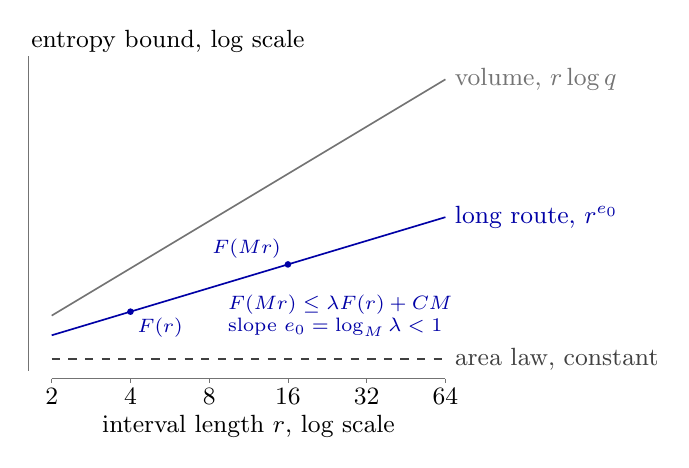
\begin{tikzpicture}[x=1cm, y=1cm, line width=0.3pt,
    lab/.style={font=\small, inner sep=1pt},
    name/.style={font=\scriptsize, text=black!55, inner sep=1pt},
    bound/.style={line width=0.6pt}]
  \def\dx{1.0}\def\dy{0.6}
  \def\xmax{5.0}\def\ymax{4.1}
  \draw[black!55] (0, 0) -- (\xmax, 0);
  \draw[black!55] (-0.3, 0.1) -- (-0.3, \ymax);
  \foreach \k/\r in {0/2, 1/4, 2/8, 3/16, 4/32, 5/64} {
    \draw[black!55] (\k*\dx, 0) -- (\k*\dx, -0.06);
    \node[lab, anchor=north] at (\k*\dx, -0.08) {\(\r\)};
  }
  \node[lab, anchor=north] at (2.5*\dx, -0.42) {interval length \(r\), log scale};
  \node[lab, anchor=south west] at (-0.3, \ymax) {entropy bound, log scale};
  \draw[bound, black!55] (0, 0.8) -- (5*\dx, {0.8 + 5*\dy});
  \node[lab, anchor=west, text=black!55] at (5*\dx + 0.08, {0.8 + 5*\dy}) {volume, \(r\log q\)};
  \draw[bound, blue!65!black] (0, 0.55) -- (5*\dx, {0.55 + 2.5*\dy});
  \node[lab, anchor=west, text=blue!65!black] at (5*\dx + 0.08, {0.55 + 2.5*\dy}) {long route, \(r^{e_0}\)};
  \draw[bound, dashed, black!75] (0, 0.25) -- (5*\dx, 0.25);
  \node[lab, anchor=west, text=black!75] at (5*\dx + 0.08, 0.25) {area law, constant};
  \fill[blue!65!black] (1*\dx, {0.55 + 0.5*\dy}) circle (1.2pt);
  \fill[blue!65!black] (3*\dx, {0.55 + 1.5*\dy}) circle (1.2pt);
  \node[name, anchor=north west, text=blue!65!black] at (1*\dx + 0.05, {0.55 + 0.5*\dy - 0.04}) {\(F(r)\)};
  \node[name, anchor=south east, text=blue!65!black] at (3*\dx - 0.05, {0.55 + 1.5*\dy + 0.04}) {\(F(Mr)\)};
  \node[name, anchor=north west, align=left, text=blue!65!black] at (2.2*\dx, 1.1)
    {\(F(Mr)\le\lambda F(r)+CM\)\\ slope \(e_0=\log_M\lambda<1\)};
\end{tikzpicture}

\end{adjustbox}
\caption{Entropy bounds for an interval of length $r$ on log–log axes (drawn with $M=4$): the volume bound $r\log q$, parallel to the diameter $r$, has slope one; the long route gives slope $e_0<1$; the area law is the constant line reached directly in the previous stage.}\label{fig:recursion}
\end{figure}

\begin{figure*}[t]
\centering
\begin{adjustbox}{max width=\linewidth}
\begin{tenkz}[lattice={1x16}, frame=plane, physical=up, bonds=none]
  \tn{} & \tn{} & \tn{} & \tn{} & \tn{} & \tn{} & \tn{} & \tn{} & \tn{} & \tn{} & \tn{} & \tn{} & \tn{} & \tn{} & \tn{} & \tn{}
  \tnmark[form=enclosure, species=selected, label pos=s]{(1,7) .. (1,10)}{$X$}
  \tnmark[form=enclosure, species=collar, label pos=n]{(1,4) .. (1,13)}{$N_{2r}(X)$}
  \tnmark[form=enclosure, species=complement, label pos=s]{(1,1) .. (1,2)}{$J$}
  \tnmark[form=enclosure, species=complement, label pos=s]{(1,15) .. (1,16)}{$J$}
\end{tenkz}

\end{adjustbox}
\caption{Amplification on the chain: the interval $X$ of length $n$, its graph neighbourhood $N_{2r}(X)$ with $r=O(n^{e_0/\alpha})=o(n)$, on which the local unitary of the amplification argument acts, and the far set $J$ it never touches, so that $I(X:J)\le n^{-M}$.}\label{fig:chain-amplify}
\end{figure*}

\begin{figure*}[t]
\centering
\begin{adjustbox}{max width=\linewidth}
\begin{tenkz}[lattice={1x16}, frame=plane, physical=up, bonds=none]
  \tn{} & \tn{} & \tn{} & \tn{} & \tn{} & \tn{} & \tn{} & \tn{} & \tn{} & \tn{} & \tn{} & \tn{} & \tn{} & \tn{} & \tn{} & \tn{}
  \tnmark[form=enclosure, species=complement, label pos=s]{(1,1) .. (1,4)}{$B$}
  \tnmark[form=enclosure, species=collar, label pos=n]{(1,5) .. (1,6)}{$D$}
  \tnmark[form=enclosure, species=selected, label pos=s]{(1,7) .. (1,7)}{$X_1$}
  \tnmark[form=enclosure, species=secondary, label pos=n]{(1,8) .. (1,9)}{$X_2$}
  \tnmark[form=enclosure, species=selected, label pos=s]{(1,10) .. (1,13)}{$X_3$}
  \tnmark[form=enclosure, species=secondary, label pos=n]{(1,14) .. (1,16)}{$X_4$}
\end{tenkz}

\end{adjustbox}
\caption{Two families on a half-line: beyond the cut and the removed sites $D$, the dyadic intervals $X_i=[2^i,2^{i+1})$ of lengths $2,4,8,\dots$ with alternating family labels, continuing to the end of the chain. Each is separated from $B$ and from all earlier same-family intervals by the previous interval, of half its length.}\label{fig:chain-families}
\end{figure*}
\notepart{The one-dimensional matrix product state approximation}{part:mps}

\section{Statement, and the two-line route}\label{sec:shortcut}

\begin{inwords}
Theorem~\ref{thm:B} asks for a single global matrix product state approximating
the ground vector, rather than an entropy bound on each cut individually.
An entropy bound alone does not yield a rank truncation because von Neumann
entropy controls only the mean of the entanglement spectrum, not the weight
of the small Schmidt eigenvalues discarded when truncating a cut; in two
dimensions, moreover, truncations across different cuts do not assemble into
a consistent tensor network, and a distributed protocol is needed to bridge
the gap. In one dimension there is a classical shortcut: if the Schmidt
spectrum across every prefix cut has a rapidly decaying tail, then
truncating the cuts sequentially from one end of the chain to the other
produces a matrix product state whose global vector error is bounded by the
sum of the square roots of the discarded tail weights (Verstraete--Cirac).
The marginal tail bound of Section~\ref{sec:tail} provides precisely such an
exponential tail at a rate $u_0$ depending only on $q,R,J/\Delta$, while the
area law fixes the mean of the spectrum. Combining the two yields
Theorem~\ref{thm:B} in a few lines, with bond dimension $CL^{4/u_0}$.

We record this sequential-truncation proof first because it is direct and
elementary. The remainder of Part~\ref{part:mps} then develops the
one-dimensional \emph{protocol} proof, which avoids sequential cut
truncations altogether and is the construction that generalises to two
dimensions.
\end{inwords}

\precisely
\begin{figure*}[t]
\centering
\begin{adjustbox}{max width=\linewidth}
\(\displaystyle \Phi\;=\;
  \begin{tenkz}[size=l, rows={wire,wire}, cols=6, bonds=none]
    \tn[at=(2,1), name=a1, skin=box, ports={0:virtual, 90:physical}]{A^{[1]}}
    \tn[at=(2,2), name=a2, skin=box, ports={180:virtual, 0:virtual, 90:physical}]{A^{[2]}}
    \tn[at=(2,3), name=a3, skin=box, ports={180:virtual, 0:virtual, 90:physical}]{A^{[3]}}
    \tn[at=(2,4), name=a4, skin=box, ports={180:virtual, 0:virtual, 90:physical}]{A^{[4]}}
    \tn[at=(2,5), name=a5, skin=box, ports={180:virtual, 0:virtual, 90:physical}]{A^{[5]}}
    \tn[at=(2,6), name=a6, skin=box, ports={180:virtual, 90:physical}]{A^{[6]}}
    \tn[at=(1,1), name=p1, skin=none, ports={270:physical, 90:physical}]{}
    \tn[at=(1,2), name=p2, skin=none, ports={270:physical, 90:physical}]{}
    \tn[at=(1,3), name=p3, skin=none, ports={270:physical, 90:physical:$q$}]{}
    \tn[at=(1,4), name=p4, skin=none, ports={270:physical, 90:physical}]{}
    \tn[at=(1,5), name=p5, skin=none, ports={270:physical, 90:physical}]{}
    \tn[at=(1,6), name=p6, skin=none, ports={270:physical, 90:physical}]{}
    \tnwire{a1.90}{p1.270} \tnwire{a2.90}{p2.270} \tnwire{a3.90}{p3.270}
    \tnwire{a4.90}{p4.270} \tnwire{a5.90}{p5.270} \tnwire{a6.90}{p6.270}
    \tnbond{a1.0}{a2.180} \tnbond{a2.0}{a3.180} \tnbond[name=d]{a3.0}{a4.180}
    \tnbond{a4.0}{a5.180} \tnbond{a5.0}{a6.180}
    \tnmark[form=label, label pos=270]{on d 0.5}{$D$}
  \end{tenkz}\)

\end{adjustbox}
\caption{A matrix product state with open boundary conditions: one tensor per site, bonds of dimension $D$ between neighbours, one physical leg per site.}\label{fig:mps-chain}
\end{figure*}

\begin{proposition}[Sequential truncation]\label{prop:VC}
Let $\Om$ be a unit vector on $\cH_\Lam$, $\Lam=\{1,\dots,L\}$. For
$1\le k\le L-1$ let $\Pi_k$ be the projection of $\cH_{[1,k]}$ onto the
span of the $\min\{D,\dim\cH_{[1,k]}\}$ eigenvectors of $\rho_{[1,k]}$ with
largest eigenvalues (so $\Pi_k=\id$ when $D\ge\dim\cH_{[1,k]}$), let $\epsilon_k=\langle\Om,(\id-\Pi_k\otimes\id)\Om\rangle$ be the discarded
mass, and put
\[
 \Phi=(\Pi_1\otimes\id)(\Pi_2\otimes\id)\cdots(\Pi_{L-1}\otimes\id)\,\Om .
\]
Then $\Phi$ is a matrix product state with open boundary conditions and
bond dimension at most $D$, and $\norm{\Phi-\Om}\le\sum_k\sqrt{\epsilon_k}$.
\end{proposition}
\begin{proof}
Write $P_k=\Pi_k\otimes\id$. Telescoping gives
$\Phi-\Om=\sum_{k=1}^{L-1}P_1\cdots P_{k-1}(P_k-\id)\Om$, and since each
prefix $P_1\cdots P_{k-1}$ is a contraction, the triangle inequality gives
$\norm{\Phi-\Om}\le\sum_k\norm{(P_k-\id)\Om}=\sum_k\sqrt{\epsilon_k}$. To
bound the bond dimension, fix a cut $k$. The intermediate vector
$P_kP_{k+1}\cdots P_{L-1}\Om$ lies in
$\operatorname{ran}\Pi_k\otimes\cH_{[k+1,L]}$ and therefore has Schmidt rank
at most $D$ across cut $k$; the remaining factors $P_1,\dots,P_{k-1}$ act
solely on $[1,k-1]$ to the left of cut $k$ and cannot increase that Schmidt
rank. A vector with Schmidt rank at most $D$ across every cut is a matrix
product state of bond dimension at most $D$.
\end{proof}

\begin{figure*}[t]
\centering
\begin{adjustbox}{max width=\linewidth}
\(\displaystyle \Phi\;=\;
  \begin{tenkz}[rows={wire,wire,wire,wire,wire}, cols=5, bonds=none]
    \tn[at=(5,1), skin=box, wide=5, name=o,
        ports={90@1:physical, 90@2:physical, 90@3:physical, 90@4:physical, 90@5:physical}]{\Omega}
    \tn[at=(4,1), skin=box, wide=4, name=p4,
        ports={270@1:physical, 270@2:physical, 270@3:physical, 270@4:physical,
               90@1:physical, 90@2:physical, 90@3:physical, 90@4:physical}]{P_4}
    \tn[at=(3,1), skin=box, wide=3, name=p3,
        ports={270@1:physical, 270@2:physical, 270@3:physical,
               90@1:physical, 90@2:physical, 90@3:physical}]{P_3}
    \tn[at=(2,1), skin=box, wide=2, name=p2,
        ports={270@1:physical, 270@2:physical, 90@1:physical, 90@2:physical}]{P_2}
    \tn[at=(1,1), skin=box, name=p1,
        ports={270:physical, 90:physical:$1$}]{P_1}
    \tn[at=(1,2), skin=none, name=t2, ports={270:physical, 90:physical:$2$}]{}
    \tn[at=(1,3), skin=none, name=t3, ports={270:physical, 90:physical:$3$}]{}
    \tn[at=(1,4), skin=none, name=t4, ports={270:physical, 90:physical:$4$}]{}
    \tn[at=(1,5), skin=none, name=t5, ports={270:physical, 90:physical:$5$}]{}
    \tnwire{o.90@1}{p4.270@1} \tnwire{o.90@2}{p4.270@2}
    \tnwire{o.90@3}{p4.270@3} \tnwire{o.90@4}{p4.270@4}
    \tnwire{p4.90@1}{p3.270@1} \tnwire{p4.90@2}{p3.270@2} \tnwire{p4.90@3}{p3.270@3}
    \tnwire{p3.90@1}{p2.270@1} \tnwire{p3.90@2}{p2.270@2}
    \tnwire{p2.90@1}{p1.270}
    \tnwire{p2.90@2}{t2.270}
    \tnwire{p3.90@3}{t3.270}
    \tnwire{p4.90@4}{t4.270}
    \tnwire{o.90@5}{t5.270}
  \end{tenkz}\)

\end{adjustbox}
\caption{Sequential truncation, drawn for $L=5$. The projector $P_k=\Pi_k\otimes 1$ onto the top $D$ Schmidt vectors of the prefix $[1,k]$ is applied for $k=L-1$ first and $k=1$ last; the output of $P_k$ lies in $\mathrm{ran}\,\Pi_k\otimes\mathcal H_{[k+1,L]}$, so across every cut the result has Schmidt rank at most $D$.}\label{fig:truncation-sequence}
\end{figure*}

\begin{theorem}[Theorem~\ref{thm:B}, two-line route]\label{thm:Bshort}
Under the hypotheses of Theorem~\ref{thm:B}, for every $L\ge2$ there is
a matrix product state $\Phi$ with bond dimension at most
$2\,\e^{C_{\mathrm{int}}}\,(32\e^{\e/2}L^4)^{1/u_0}$ and
$\min_\theta\norm{\Phi/\norm\Phi-\e^{i\theta}\Om}\le L^{-1}$, where $u_0$ is
\eqref{eq:theta} and $C_{\mathrm{int}}$ is \eqref{eq:final}.
\end{theorem}
\begin{proof}
Fix a cut $k$ and put $X=[1,k]$. By Lemma~\ref{lem:tail}, the eigenvalues
$p$ of $\rho_X$ with $-\log p>S(X)+w$ have total mass at most
$2\e^{\e/2}\e^{-u_0w}$, while the eigenvalues with $-\log p\le S(X)+w$ each
satisfy $p\ge\e^{-S(X)-w}$ and therefore number at most $\e^{S(X)+w}$.
Choose $w$ so that $2\e^{\e/2}\e^{-u_0w}=(16L^4)^{-1}$ and set
$D=\lceil\e^{C_{\mathrm{int}}+w}\rceil\ge\e^{S(X)+w}$ by Theorem~\ref{thm:A}.
Then $\epsilon_k\le(16L^4)^{-1}$ for every $k$, and Proposition~\ref{prop:VC}
gives $\norm{\Phi-\Om}\le(L-1)/(4L^2)\le1/(4L)$. In particular $\Phi\ne0$
and $\norm{\Phi/\norm\Phi-\Om}\le2\norm{\Phi-\Om}\le L^{-1}$. The bond
dimension satisfies $D\le2\e^{C_{\mathrm{int}}+w}$ with
$\e^{w}=(32\e^{\e/2}L^4)^{1/u_0}$.
\end{proof}

\begin{remark}
The exponent $4/u_0$ is of order $\sqrt{(1+J/\Delta)\cB_R}$. Whereas
Hastings' original construction yields a polynomial bond dimension whose
exponent is exponential in $J/\Delta$, the marginal tail bound gives a
square-root dependence on $J/\Delta$. This exponent is a feature of the
direct sequential-truncation route rather than of the protocol below.
\end{remark}

\subsection*{Plan of the protocol route}

\begin{inwords}
The distributed protocol proof has four layers:
\begin{enumerate}[leftmargin=2em]
\item \emph{Information at logarithmic separation.} Two regions of the
chain separated by $D\log L$ sites share at most $L^{-p}$ nats of mutual
information. This is where the protocol route uses the
spectral gap. In two dimensions, establishing logarithmic
separation requires a coarse collar bound, a cell conditional-information
lemma, and an angular induction; in one dimension, it follows directly from
the area law and a single two-replica information-reset lemma
(Section~\ref{sec:logsep}).
\item \emph{Ownership moves.} Three elementary operations redistribute site
registers among parties while keeping the global state close to a reference
state: a \emph{birth} (handing an interior interval to a new owner), its
reverse, a \emph{death}, and an \emph{exchange} of ownership assignments
between two copies of the ground state inside a window. Each move is a
contraction built from private maps and at most one normalised shared
bipartite vector or covector, and each incurs $O(L^{-p/2})$ vector error
whenever the moved region has mutual information at most $L^{-p}$ with all
third-party registers (Section~\ref{sec:moves}).
\item \emph{The sweep schedule.} A left-to-right sweep with a moving
remainder party creates the logarithmic block owners one by one. The only
obstruction is dissolving a narrow remainder band wedged between two
distinct neighbouring owners; this is accomplished by a fixed sequence of
moves using an auxiliary copy of the ground state, copied from the edge
construction of the two-dimensional paper \cite{PP}, so that every party
participates in a bounded number of moves (Section~\ref{sec:sweep}).
\item \emph{Compression and assembly.} The sweep is a linear calculation
whose intermediate private registers have arbitrarily large dimension.
Replacing each shared bipartite resource in the density calculation by an
empirical average of polynomially many random product operators approximates
the output physical density in trace norm; the error bound is independent
of the private dimensions because each party participates in boundedly many
gates. Extracting a single computational-basis column of the resulting
operator network and placing its nodes along the chain yields the matrix
product state (Sections~\ref{sec:compression}, \ref{sec:routing}).
\end{enumerate}
\end{inwords}

\section{Information at logarithmic separation}\label{sec:logsep}

\subsection{Purifications, fidelity, and splitting}

\begin{inwords}
To change the ownership of a region $T$ without disturbing the global state,
we must decouple $T$ from the registers $E$ held by third parties using an
operation supported entirely on the separating buffer $U=\Lam\setminus(T\cup E)$.
Small mutual information $I(T:E)$ means that the reduced state $\rho_{TE}$
is close in relative entropy to the product state $\rho_T\otimes\rho_E$.
Relative entropy controls Uhlmann fidelity, which equals the maximum overlap
between purifications. Since $U$ purifies $TE$ in the pure ground state
$\Om$, Uhlmann's theorem guarantees an isometry $V$ acting on the buffer
$U$ alone that maps $\Om$ into nearly a tensor product $s\otimes s'$ of a
purification of $\rho_T$ and a purification of $\rho_E$. Any party holding
$U$ can execute this decoupling privately; this single mechanism underlies
all births, deaths, and exchanges.
\end{inwords}

\precisely
For density operators $\rho,\sigma$ put $F(\rho,\sigma)=\norm{\sqrt\rho\sqrt\sigma}_1$
and $D(\rho\|\sigma)=\Tr\rho(\log\rho-\log\sigma)$, taken to be infinite
when the support of $\rho$ is not contained in that of $\sigma$.

\begin{lemma}[Fidelity, information, Uhlmann]\label{lem:fidelity}
For normalised finite-dimensional states, $F(\rho,\sigma)\ge\e^{-D(\rho\|\sigma)/2}$,
and $D(\rho_{AC}\|\rho_A\otimes\rho_C)=I(A:C)$. If $\xi$ purifies $\rho$ on
$\cH\otimes\cK$ and $\eta$ purifies $\sigma$ on $\cH\otimes\cK'$, then after
enlarging $\cK'$ if necessary there is an isometry $V:\cK\to\cK'$ with
$\abs{\langle\eta,(\id\otimes V)\xi\rangle}=F(\rho,\sigma)$.
\end{lemma}
\begin{proof}
Let $(p_i,\ket i)$ and $(q_j,\ket{j'})$ be eigenpairs of $\rho$ and $\sigma$.
If $D(\rho\|\sigma)<\infty$, then $w_{ij}=p_i\abs{\langle i|j'\rangle}^2$ defines
a probability distribution on the pairs with $p_iq_j>0$, and
$D(\rho\|\sigma)=\sum_{ij}w_{ij}\log(p_i/q_j)$. By convexity of the exponential,
$\Tr\sqrt\rho\sqrt\sigma=\sum_{ij}w_{ij}\exp(-\tfrac12\log(p_i/q_j))\ge\e^{-D(\rho\|\sigma)/2}$,
and the trace norm dominates the trace. The identity
$D(\rho_{AC}\|\rho_A\otimes\rho_C)=I(A:C)$ follows from expanding
$\log(\rho_A\otimes\rho_C)$. The purification statement is Uhlmann's
theorem: the overlaps $\Tr(\sqrt\rho\sqrt\sigma U)$ over unitaries $U$ on a
common purifying space have maximum modulus $\norm{\sqrt\rho\sqrt\sigma}_1$
by polar decomposition, and any two purifications of the same state are
related by an isometry on the purifying factor.
\end{proof}

\begin{lemma}[Splitting]\label{lem:splitting}
Let $T,U,E$ partition $\Lam$ and $b=I_\Om(T:E)$. There are finite-dimensional
spaces $\cB_T,\cB_E$, an isometry $V:\cH_U\to\cB_T\otimes\cB_E$ and unit vectors
$s\in\cH_T\otimes\cB_T$, $s'\in\cH_E\otimes\cB_E$ with
\[
 \norm{(\id_{TE}\otimes V)\Om-s\otimes s'}\le\sqrt{2(1-\e^{-b/2})}\le\sqrt b .
\]
\end{lemma}
\begin{proof}
Because $\rho_{TE}$ is supported in $\supp\rho_T\otimes\supp\rho_E$ (the
projector onto the kernel of a marginal, tensored with the identity, has
zero expectation in the positive joint state), the relative entropy
$D(\rho_{TE}\|\rho_T\otimes\rho_E)=b$ is finite. Choose purifications $s$
of $\rho_T$ and $s'$ of $\rho_E$, enlarge their purifying spaces so that
$\cB_T\otimes\cB_E$ contains an isometric copy of $\cH_U$, and apply
Lemma~\ref{lem:fidelity}: there is an isometry $V$ on $\cH_U$ such that
$(\id_{TE}\otimes V)\Om$ has real overlap at least $\e^{-b/2}$ with
$s\otimes s'$. Two unit vectors with real overlap $F$ have Euclidean
distance $\sqrt{2(1-F)}$.
\end{proof}

\begin{figure}[t]
\centering
\begin{adjustbox}{max width=\linewidth}
\(\begin{tenkz}[size=l, rows={wire,wire}, cols=4, bonds=none]
  \tn[at=(2,1), skin=box, wide=4, name=o, ports={90@1:physical:$T$, 90@2:physical, 90@4:physical:$E$}]{\Omega}
  \tn[at=(1,2), skin=box, wide=2, name=v, ports={270@1:physical, 90@1:physical, 90@2:physical}]{V}
  \tnwire{o.90@2}{v.270@1}
\end{tenkz}
\approx
\begin{tenkz}[size=l, rows={wire}, cols=4, bonds=none]
  \tn[at=(1,1), skin=box, wide=2, ports={90@1:physical:$T$, 90@2:physical}]{s}
  \tn[at=(1,3), skin=box, wide=2, ports={90@1:physical, 90@2:physical:$E$}]{s'}
\end{tenkz}\)

\end{adjustbox}
\caption{The splitting lemma as a diagram: the isometry $V$ on the buffer $U$ turns $\Om$ into nearly a product of a purification $s$ of $\rho_T$ and a purification $s'$ of $\rho_E$.}\label{fig:split}
\end{figure}

\subsection{The information reset}\label{sec:reset}

\begin{inwords}
The area law gives $I(R:C)=O(1)$ between an interval $R$ and any disjoint
region $C$, never $o(1)$. To assemble a global tensor network from local
operations across the chain, however, errors must be suppressed to an
arbitrary inverse power $L^{-p}$ so that they remain small when summed over
$O(L)$ steps. The information-reset lemma bridges this gap by shrinking $R$
and $C$ inward to cores $R_0\subseteq R$ and $C_0\subseteq C$ separated from
their outer boundaries by a margin of width $w=O(\log L)$.

The physical mechanism is a two-replica swap. Take two identical copies of
the ground vector, $\Psi=\Om\otimes\Om$, and swap the two copies on $R$ to
obtain $\Phi=F_R\Psi$. In the first replica of $\Phi$, the core $R_0\subseteq R$
has been swapped in from the second copy of $\Om$ while $C_0\subseteq C$
remains from the first, so the two cores originate from independent copies and
have the exact product marginal $\rho_{R_0}\otimes\rho_{C_0}$. If a unitary $U$
supported entirely in the buffer region between $R_0$ and $C_0$ maps $\Psi$
to $\Phi$ up to error $O(L^{-r_*})$, then the joint marginal of the cores in
$\Psi$ agrees with $\rho_{R_0}\otimes\rho_{C_0}$ up to $O(L^{-r_*})$, which
implies $I_\Om(R_0:C_0)\le L^{-p}$.

The unitary $U$ is constructed in three steps. First, the bound $I(R:C)\le b$
and the splitting lemma produce a Hermitian contraction $W$ on the buffer
$Q=\Lam\setminus(R\cup C)$ of both copies with macroscopic overlap
$z=\langle\Phi,W\Psi\rangle\ge\e^{-2b}$. Because $W\Psi$ still carries excited
components, $W$ is not yet close to a unitary mapping $\Psi$ to $\Phi$.
Second, a two-sided Gaussian spectral filter,
$M=\int g_h(t)\e^{it\mathbb H'}W\e^{-it\mathbb H}dt$, damps out excited states
in both directions, projecting $W\Psi$ onto $z\Phi$ and $W^\dagger\Phi$ onto
$z\Psi$ with error $\e^{-h\Delta^2/2}$, because $\Psi$ and $\Phi$ are the unique
gapped ground vectors of the doubled Hamiltonians $\mathbb H$ and
$\mathbb H'=F_R\mathbb HF_R$. Third, because time evolution spreads operator
supports, a Lieb--Robinson bound localises $M$ to within distance
$\ell=O(1+b+\log L)$ of the buffer $Q$ and of the boundary zone $Z_R$ where
$\mathbb H$ and $\mathbb H'$ differ. Rescaling the localised operator makes it
almost isometric on $\Psi$, and its polar unitary $U$ remains supported strictly
outside both cores. The lemma is proved exactly as in the two-dimensional
source; we only insert the one-dimensional locality bound.
\end{inwords}

\precisely
To control the spatial spread of the Gaussian filter, we first record the standard
Lieb--Robinson propagation estimate on the doubled chain. Let
$\mathbb H$ be a Hamiltonian on $\bigotimes_{x\in\Lam}(\C^q\otimes\C^q)$
written as a sum of terms $k_Z$ supported on sets $Z$ of diameter at most
$R$ with $\sum_{Z\ni x}\norm{k_Z}\le b_0$ for every $x$, and let
$\tau_t(A)=\e^{it\mathbb H}A\e^{-it\mathbb H}$.

\begin{lemma}[Lieb--Robinson bound on a chain]\label{lem:LR}
There are $C,v,\mu>0$ depending only on $R$ and $b_0$ such that for every
operator $A$ supported in $S\subseteq\Lam$, every site $y$, and every
operator $B_y$ supported at $y$,
\[
 \norm{[\tau_t(A),B_y]}\le C\abs S\,\norm A\,\norm{B_y}\,\e^{v\abs t-\mu\,\dist(S,y)} .
\]
Consequently, if $\mathcal P_D$ denotes the conditional expectation onto
operators supported in $D$ (the average over independent Haar unitaries at
the sites outside $D$), then for every $\ell\ge0$,
\[
 \norm{\tau_t(A)-\mathcal P_{N_\ell(S)}\tau_t(A)}\le C'\abs S^2\,\norm A\,\e^{v\abs t-\mu\ell}.
\]
\end{lemma}
\begin{proof}
For $t\ge0$ put $c_y(S,t)=\sup\{\norm{[\tau_t(A),B_y]}:\supp A\subseteq S,\norm A\le1\}$.
Differentiating and using the Jacobi identity shows that $\frac{d}{dt}[\tau_t(A),B_y]$
equals $i[\sum_{Z\cap S\ne\varnothing}\tau_t(k_Z),[\tau_t(A),B_y]]$
plus a sum over $Z\cap S\ne\varnothing$ of $-i[\tau_t(A),[\tau_t(k_Z),B_y]]$. The
first term is removed by a unitary change of frame, yielding the integral inequality
$c_y(S,t)\le c_y(S,0)+2\sum_{Z\cap S\ne\varnothing}\norm{k_Z}\int_0^tc_y(Z,u)\,du$.
Iterating this inequality, and using the trivial bound $c_y(Z,u)\le2\norm{B_y}$ to see
that the remainder after $m$ iterations vanishes as $m\to\infty$, gives
\[
 c_y(S,t)\le 2\norm{B_y}\sum_{m\ge0}\frac{(2t)^m}{m!}
 \sum_{\substack{Z_1\cap S\ne\varnothing,\ Z_{i+1}\cap Z_i\ne\varnothing\\ y\in Z_m}}
 \prod_{i=1}^m\norm{k_{Z_i}},
\]
with the $m=0$ term equal to $\mathbf 1_{\{y\in S\}}$. Since the norms of
the interaction terms meeting any set of $n$ sites sum to at most $nb_0$, the inner
sum is at most $\abs S\,b_0\,((R+1)b_0)^{m-1}\le\abs S\kappa^m$ with
$\kappa=(R+1)b_0$. Moreover, a chain of $m$ supports of diameter at most $R$
connecting $S$ to $y$ requires $mR\ge\dist(S,y)$. Hence,
for every $\mu>0$,
$c_y(S,t)\le 2\abs S\norm{B_y}\e^{-\mu\dist(S,y)}\sum_m(2\kappa\e^{\mu R}t)^m/m!$,
which gives the first bound with $v=2\kappa\e^{\mu R}$; negative times are
identical. For the second
bound, expressing $\mathcal P_D$ as a product of commuting single-site Haar twirls
$T_y$ and telescoping gives
$\norm{B-\mathcal P_DB}\le\sum_{y\notin D}\sup_{U_y}\norm{[B,U_y]}$. Because at most
$2\abs S$ sites lie at each distance $d>\ell$ from $S$, the sum is bounded by
$4C\abs S^2\norm A\e^{vt}\sum_{d>\ell}\e^{-\mu d}$.
\end{proof}

\begin{figure*}[t]
\centering
\begin{adjustbox}{max width=\linewidth}
\begin{tenkz}[lattice={1x20}, frame=plane, physical=up, bonds=none]
  \tn{} & \tn{} & \tn{} & \tn{} & \tn{} & \tn{} & \tn{} & \tn{} & \tn{} & \tn{} & \tn{} & \tn{} & \tn{} & \tn{} & \tn{} & \tn{} & \tn{} & \tn{} & \tn{} & \tn{}
  \tnmark[form=enclosure, species=selected, label pos=s]{(1,5) .. (1,7)}{$R_0$}
  \tnmark[form=enclosure, species=secondary, label pos=n]{(1,3) .. (1,9)}{$R$}
  \tnmark[form=enclosure, species=collar, label pos=s]{(1,1) .. (1,2)}{$Q$}
  \tnmark[form=enclosure, species=collar, label pos=s]{(1,10) .. (1,12)}{$Q$}
  \tnmark[form=enclosure, species=complement, label pos=n]{(1,13) .. (1,20)}{$C$}
  \tnmark[form=enclosure, species=selected, label pos=s]{(1,15) .. (1,20)}{$C_0$}
  \tnmark[form=bracket, species=secondary, label pos=s]{(1,3) .. (1,4)}{$w$}
  \tnmark[form=bracket, species=secondary, label pos=s]{(1,8) .. (1,9)}{$w$}
  \tnmark[form=bracket, species=complement, label pos=s]{(1,13) .. (1,14)}{$w$}
  \tnmark[form=enclosure, species=neutral, tint, label pos=n]{(1,1) .. (1,3)}{$S$}
  \tnmark[form=enclosure, species=neutral, tint, label pos=n]{(1,9) .. (1,14)}{$S=N_\ell(Q\cup Z_R)$}
\end{tenkz}

\end{adjustbox}
\caption{The reset geometry, drawn in one replica of $\Psi=\Omega\otimes\Omega$: the cores $R_0\subset R$ and $C_0\subset C$, the buffer $Q=\Lambda\setminus(R\cup C)$, the margins of width $w$, the set $Z_R$ near the cut edges of $R$, and the support $S=N_\ell(Q\cup Z_R)$ of the unitary, which stays clear of both cores.}\label{fig:chain-reset}
\end{figure*}

\begin{lemma}[Information reset]\label{lem:reset}
For every $p>0$ there is $C_p<\infty$, depending only on $p,q,R,J,\Delta$,
with the following property for all sufficiently large $L$. Let
$R,C\subseteq\Lam$ be disjoint, $R_0\subseteq R$, $C_0\subseteq C$, and
suppose $I_\Om(R:C)\le b$. If
\[
\begin{split}
 &\dist(R_0,\Lam\setminus R)>w,\qquad \dist(C_0,\Lam\setminus C)>w,\\
 &w=C_p(1+b+\log L),
\end{split}
\]
then $I_\Om(R_0:C_0)\le L^{-p}$.
\end{lemma}
\begin{proof}
If either core is empty there is nothing to prove. Let $\Psi=\Om\otimes\Om$ on
two replicas, $F_R$ be the unitary exchanging the two replicas at the sites
of $R$, $\Phi=F_R\Psi$, and $Q=\Lam\setminus(R\cup C)$.

\emph{Overlap.} Apply Lemma~\ref{lem:splitting} to $(T,U,E)=(R,Q,C)$ to obtain an
isometry $V:\cH_Q\to\cB_R\otimes\cB_C$ and unit vectors $a\in\cH_R\otimes\cB_R$,
$a'\in\cH_C\otimes\cB_C$ satisfying
$\abs{\langle a\otimes a',\widetilde\Om\rangle}\ge\e^{-b/2}$, where
$\widetilde\Om=(\id\otimes V)\Om$. The largest Schmidt probability (marginal eigenvalue) of
$\widetilde\Om$ across the bipartition $R\cB_R\,|\,C\cB_C$ is therefore at least $\e^{-b}$,
so $\Tr\rho_{\widetilde\Om,R\cB_R}^2\ge\e^{-2b}$. On the two
replicas of $Q$, define the Hermitian contraction
$W=(V^\dagger\otimes V^\dagger)F_{\cB_R}(V\otimes V)$, where $F_{\cB_R}$ swaps
the two copies of $\cB_R$. Since $V$ acts outside $R$, the replica-swap identity
$\langle\xi^{\otimes2},F_{A}\xi^{\otimes2}\rangle=\Tr\rho_{\xi,A}^2$ gives
\begin{equation}\label{eq:zoverlap}
\begin{split}
 &z:=\langle\Phi,W\Psi\rangle=\langle\widetilde\Om^{\otimes2},F_RF_{\cB_R}\widetilde\Om^{\otimes2}\rangle\\
 &\qquad=\Tr\rho_{\widetilde\Om,R\cB_R}^2\ \ge\ \e^{-2b}.
\end{split}
\end{equation}

\emph{Two-sided Gaussian filtering.} Let $\mathbb H=H\otimes\id+\id\otimes H$
and $\mathbb H'=F_R\mathbb HF_R$. Both are range-$R$ Hamiltonians on the
doubled chain with uniformly bounded interaction sums, unique ground
vectors $\Psi$ and $\Phi$, common ground energy $\mathcal E=2E_0$, and spectral gap at
least $\Delta$. Their difference $\mathbb H'-\mathbb H$ is a sum of at most $N_R\abs{\partial R}$
terms of norm at most $2J$, namely those terms of $\mathbb H$ whose support meets both $R$
and $\Lam\setminus R$ (terms supported entirely inside $R$ are merely exchanged between the
two identical replicas); let $Z_R$ be the union of their supports, which lies
within distance $R$ of the cut edges of $R$. Put
$B_*=1+b+\log L$, $r_*=2p+10$, and $h=AB_*$ with $A\Delta^2/2\ge r_*+30$, and define
\[
\begin{split}
 &g_h(t)=(2\pi h)^{-1/2}\e^{-t^2/(2h)},\\
 &M=\int_{\R}g_h(t)\,\e^{it\mathbb H'}W\e^{-it\mathbb H}\,dt .
\end{split}
\]
The operator $M$ is a contraction, and by the spectral theorem
$M\Psi=\e^{-h(\mathbb H'-\mathcal E)^2/2}W\Psi$ and $M^\dagger\Phi=\e^{-h(\mathbb H-\mathcal E)^2/2}W^\dagger\Phi$.
Because $\mathbb H'$ and $\mathbb H$ have gap at least $\Delta$ above $\mathcal E$,
\begin{equation}\label{eq:twosided}
 \norm{M\Psi-z\Phi},\ \norm{M^\dagger\Phi-z\Psi}\le\e^{-h\Delta^2/2}\le\e^{-10b}L^{-r_*}.
\end{equation}
Truncating the time integral to $\abs t\le T=T_0B_*$ incurs an error of at most
$2\e^{-T_0^2B_*/(2A)}$, which is likewise at most $\e^{-10b}L^{-r_*}$ once
$T_0^2/(2A)\ge r_*+30$.

\emph{Localisation.} Factor the integrand as
$\e^{it\mathbb H'}W\e^{-it\mathbb H}=(\e^{it\mathbb H'}W\e^{-it\mathbb H'})\,V(t)$
with $V(t)=\e^{it\mathbb H'}\e^{-it\mathbb H}$, whose left generator
$G(t)=\e^{it\mathbb H'}(\mathbb H'-\mathbb H)\e^{-it\mathbb H'}$ is a sum of
the boundedly many terms supported in $Z_R$. Applying Lemma~\ref{lem:LR} to $W$ (supported in $Q$, of norm at most $1$)
and to each term of $G(t)$ yields Hermitian localised approximants
$W_\ell(t)=\mathcal P_{N_\ell(Q)}\bigl(\e^{it\mathbb H'}W\e^{-it\mathbb H'}\bigr)$
and $G_\ell(t)=\mathcal P_{N_\ell(Z_R)}G(t)$ satisfying
\[
 \norm{\e^{it\mathbb H'}W\e^{-it\mathbb H'}-W_\ell(t)}+\norm{G(t)-G_\ell(t)}\le CL^2\,\e^{v\abs t-\mu\ell},
\]
where the factor $L^2$ bounds $\abs Q^2$ and $\abs{\partial R}$. Let
$V_\ell(t)$ be the unitary evolution generated by $G_\ell(t)$, which is supported in
$N_\ell(Z_R)$; Duhamel's formula gives $\norm{V(t)-V_\ell(t)}\le CL^2\abs t\e^{v\abs t-\mu\ell}$.
Consequently, $W_\ell(t)V_\ell(t)$ is a contraction supported in
$S:=N_\ell(Q\cup Z_R)$ that approximates the integrand uniformly for
$\abs t\le T$ with error at most $CL^2(1+T)\e^{vT-\mu\ell}$. Choose
$\ell=\lceil K_{\mathrm{loc}}B_*\rceil$ with $K_{\mathrm{loc}}$ fixed large
enough (after $T_0$) that this error is at most $\e^{-10b}L^{-r_*}$,
using $\log L\le B_*$ and $\log(1+T)\le C+B_*$. Averaging the localised
integrands against the truncated Gaussian yields a contraction
$M_{\mathrm{loc}}$ supported in $S$ with
\begin{equation}\label{eq:loctwosided}
 \norm{M_{\mathrm{loc}}\Psi-z\Phi},\ \norm{M_{\mathrm{loc}}^\dagger\Phi-z\Psi}\le C\e^{-10b}L^{-r_*}.
\end{equation}

\emph{Polar decomposition.} Rescale by setting $D=M_{\mathrm{loc}}/z$. Since $z\ge\e^{-2b}$, we have $\norm D\le\e^{2b}$ and
$\norm{D\Psi-\Phi},\norm{D^\dagger\Phi-\Psi}\le C\e^{-8b}L^{-r_*}$. Writing
$(D^\dagger D-\id)\Psi=D^\dagger(D\Psi-\Phi)+(D^\dagger\Phi-\Psi)$ then gives
$\norm{(D^\dagger D-\id)\Psi}\le C\e^{-6b}L^{-r_*}$. Because $D$ acts on the finite-dimensional space $\cH_S$, its polar partial
isometry extends to a unitary $U$ on
$\cH_S$ tensored with the
identity outside $S$. Using the scalar inequality $(\sqrt x-1)^2\le(x-1)^2$ for $x\ge0$, we obtain
$\norm{(U-D)\Psi}=\norm{(\id-\abs D)\Psi}\le\norm{(\id-D^\dagger D)\Psi}$, and therefore
\begin{equation}\label{eq:Uerror}
 \norm{U\Psi-\Phi}\le C\e^{-6b}L^{-r_*}\le CL^{-r_*}.
\end{equation}

\emph{Support and conclusion.} By hypothesis, every site of $Q$ lies at distance greater than $w$ from
both $R_0$ and $C_0$. Any interaction term whose support meets both $R$ and $\Lam\setminus R$
contains a site $y\notin R$ (at distance greater than $w$ from $R_0$) and a site
$x\in R\subseteq\Lam\setminus C$ (at distance greater than $w$ from $C_0$); since its support
has diameter at most $R$, every site of $Z_R$ lies at distance greater than $w-R$ from
both cores. Choosing $C_p>K_{\mathrm{loc}}+R+3$ ensures that $S=N_\ell(Q\cup Z_R)$ is
disjoint from $R_0\cup C_0$ in both replicas. Thus $U$ leaves the
two-replica marginal on $R_0C_0$ unchanged. In $\Phi=F_R\Psi$, the marginal on
$R_0C_0$ of the \emph{first} replica is $\rho_{R_0}\otimes\rho_{C_0}$,
because $R_0$ is swapped in from the second replica whereas $C_0$ remains in the first. By
\eqref{eq:Uerror} and the contractivity of the partial trace, the ground-state
marginal $\rho_{R_0C_0}$ lies within trace distance $CL^{-r_*}$ of
$\rho_{R_0}\otimes\rho_{C_0}$. Applying the Alicki--Fannes--Winter continuity bound
$\abs{S(A|B)_\rho-S(A|B)_\sigma}\le C\sqrt\delta\log(\e\dim\cH_A)$ with
$\delta=\frac12\norm{\rho-\sigma}_1$ \cite{Winter2016} to
$I(R_0:C_0)=S(R_0)-S(R_0|C_0)$, and using $\log\dim\cH_{R_0}\le L\log q$, gives
$I_\Om(R_0:C_0)\le CL^{1-r_*/2}=CL^{-p-4}\le L^{-p}$ for all sufficiently large $L$.
\end{proof}

\begin{figure*}[t]
\centering
\begin{adjustbox}{max width=\linewidth}
\(\displaystyle \Phi=F_R\Psi\;=\;
  \begin{tenkz}[rows={wire,wire}, cols=7, bonds=none]
    \tn[at=(2,1), skin=box, wide=3, name=o1,
        ports={90@1:physical:$C$, 90@2:physical:$Q$, 90@3:physical}]{\Omega}
    \tn[at=(2,5), skin=box, wide=3, name=o2,
        ports={90@1:physical, 90@2:physical:$Q$, 90@3:physical:$C$}]{\Omega}
    \tn[at=(1,3), skin=box, wide=3, name=f,
        ports={270@1:physical, 270@3:physical, 90@1:physical:$R$, 90@3:physical:$R$}]{F_R}
    \tnwire{o1.90@3}{f.270@1}
    \tnwire{o2.90@1}{f.270@3}
  \end{tenkz}
  \;=\;
  \begin{tenkz}[rows={wire,wire}, cols=7, bonds=none]
    \tn[at=(2,1), skin=box, wide=3, name=o1,
        ports={90@1:physical:$C$, 90@2:physical:$Q$, 90@3:physical}]{\Omega}
    \tn[at=(2,5), skin=box, wide=3, name=o2,
        ports={90@1:physical, 90@2:physical:$Q$, 90@3:physical:$C$}]{\Omega}
    \tn[at=(1,3), skin=none, name=r1, ports={270:physical, 90:physical:$R$}]{}
    \tn[at=(1,5), skin=none, name=r2, ports={270:physical, 90:physical:$R$}]{}
    \tnwire[name=a]{o1.90@3}{r2.270}
    \tnwire[name=b, cross={under at crossing of a and b}]{o2.90@1}{r1.270}
  \end{tenkz}\)

\end{adjustbox}
\caption{The swap $F_R$ exchanges the two copies of $\Omega$ on $R$ only (the first copy is drawn mirrored so that the two $R$ legs are adjacent). In $\Phi=F_R\Psi$ the core $R_0$ of the first copy comes from the second copy while $C_0$ does not, so the first copy's marginal on $R_0C_0$ is $\rho_{R_0}\otimes\rho_{C_0}$.}\label{fig:replica-swap}
\end{figure*}

\begin{figure*}[t]
\centering
\begin{adjustbox}{max width=\linewidth}
\(\displaystyle M=\int_{\mathbb R}g_h(t)\,dt\;
  \begin{quantikz}[row sep={0.55cm,between origins}]
    \lstick{$R^{(1)}$} & \gate[6]{e^{-it\mathbb H}} & & \gate[6]{e^{it\mathbb H'}} & \\
    \lstick{$R^{(2)}$} & & & & \\
    \lstick{$Q^{(1)}$} & & \gate[2]{W} & & \\
    \lstick{$Q^{(2)}$} & & & & \\
    \lstick{$C^{(1)}$} & & & & \\
    \lstick{$C^{(2)}$} & & & &
  \end{quantikz}\)

\end{adjustbox}
\caption{The two-sided Gaussian filter: evolve with the doubled Hamiltonian, apply $W$ on the two copies of the buffer, evolve back with the swapped Hamiltonian, and average against a Gaussian in time. It sends $W\Psi$ to a multiple of $\Phi$ and $W^\dagger\Phi$ to a multiple of $\Psi$, up to $e^{-h\Delta^2/2}$.}\label{fig:qc-gaussian-filter}
\end{figure*}

\subsection{The one-dimensional separation lemma}\label{sec:logsep2}

\begin{inwords}
Combining the one-dimensional area law with the information reset yields
polynomial decoupling at logarithmic separation. By Theorem~\ref{thm:A}, any
interval $R$ (or union of $k_0$ intervals) has entanglement entropy at most
$k_0C_{\mathrm{int}}$, so its mutual information with any disjoint region $C$
is bounded by the constant $2k_0C_{\mathrm{int}}$. Feeding this uniform bound
into Lemma~\ref{lem:reset} shows that any union $T$ of at most $k_0$ intervals
and any set $E$ separated from $T$ by a distance of order $\log L$ satisfy
$I_\Om(T:E)\le L^{-p}$. Because the one-dimensional area law bounds interval
entropies uniformly at every scale, this single step establishes logarithmic
decoupling for intervals of arbitrary length, from a few sites up to the
entire chain. This replaces the entire Section~3 of the two-dimensional
paper (coarse collar, cell conditional information, angular induction).
\end{inwords}

\precisely
\begin{lemma}[Information at logarithmic separation]\label{lem:logsep}
For every $p>0$ and $k_0\ge1$ there is $D_p=D_p(q,R,J,\Delta,k_0)$ such that for
all sufficiently large $L$, every $T\subseteq\Lam$ that is a union of at most
$k_0$ intervals, and every $E\subseteq\Lam$ with $\dist(T,E)\ge D_p\log L$,
\[
 I_\Om(T:E)\le L^{-p}.
\]
\end{lemma}
\begin{proof}
Let $b=4k_0C_{\mathrm{int}}$, let $w=C_p(1+b+\log L)$ be the margin width from Lemma~\ref{lem:reset},
and choose $D_p$ so that $D_p\log L\ge 3w+3$. Put $R=T^{+(w+1)}$ (a union of at most $k_0$
intervals), $C=\Lam\setminus T^{+(2w+2)}$, $R_0=T$, and $C_0=E$. Then
$\dist(R_0,\Lam\setminus R)\ge w+1$ and $\dist(C_0,\Lam\setminus C)\ge w+1$. Moreover,
$I(R:C)\le 2S(R)\le 2k_0C_{\mathrm{int}}\le b$ by Theorem~\ref{thm:A},
using subadditivity across the at most $k_0$ intervals of $R$ together with
$I(R:C)=S(R)+S(C)-S(RC)\le 2S(R)$ from the Araki--Lieb inequality.
Applying Lemma~\ref{lem:reset} gives $I_\Om(T:E)\le L^{-p}$.
\end{proof}

\begin{figure*}[t]
\centering
\begin{adjustbox}{max width=\linewidth}
\begin{tenkz}[lattice={1x18}, frame=plane, physical=up, bonds=none]
  \tn{} & \tn{} & \tn{} & \tn{} & \tn{} & \tn{} & \tn{} & \tn{} & \tn{} & \tn{} & \tn{} & \tn{} & \tn{} & \tn{} & \tn{} & \tn{} & \tn{} & \tn{}
  \tnmark[form=enclosure, species=selected, label pos=s]{(1,8) .. (1,10)}{$T$}
  \tnmark[form=enclosure, species=secondary, label pos=n]{(1,6) .. (1,12)}{$R=T^{+(w+1)}$}
  \tnmark[form=enclosure, species=complement, label pos=n]{(1,1) .. (1,3)}{$C$}
  \tnmark[form=enclosure, species=complement, label pos=n]{(1,15) .. (1,18)}{$C$}
  \tnmark[form=enclosure, species=collar, label pos=s]{(1,1) .. (1,2)}{$E$}
  \tnmark[form=enclosure, species=collar, label pos=s]{(1,17) .. (1,18)}{$E$}
  \tnmark[form=bracket, species=collar, label pos=s]{(1,3) .. (1,7)}{$D_p\log L$}
\end{tenkz}

\end{adjustbox}
\caption{The separation lemma: an interval $T$, its enlargement $R$, the far region $C$ and the set $E\subseteq C$ at distance $D_p\log L$ from $T$. The area law bounds $I(R:C)$ by a constant and the reset makes $I(T:E)\le L^{-p}$.}\label{fig:chain-logsep}
\end{figure*}

\begin{remark}[A route without Lieb--Robinson bounds]\label{rem:LRfree}
The information-reset lemma is the only place in Part~\ref{part:mps} where a
Lieb--Robinson bound is invoked. It can be replaced by the algebraic amplification
argument of \cite[Section~10]{AL}, which uses exact positive quasi-local
constraints with stretched-exponential tails $\e^{-cl^\alpha}$
($\alpha=p/(p+1)$), random products of the associated contractions, and a
polar decomposition, without requiring a propagation bound for the unitary
dynamics. With the area law as input, that argument yields
$I(T:E)\le L^{-M}$ whenever $E$ lies beyond distance $C(\log L)^{1/\alpha}$ of an
interval $T$. Running the protocol below on blocks of that width produces
a matrix product state of bond dimension $\exp(O((\log L)^{1/\alpha}))$, which is
quasi-polynomial for every fixed $p$ and approaches polynomial only in the large-$p$ limit.
Achieving strictly polynomial bond dimension through the protocol route relies on the
logarithmic separation provided by Lemma~\ref{lem:logsep}.
\end{remark}
\section{Distributed constructions and the three moves}\label{sec:moves}

\begin{inwords}
To convert logarithmic decoupling into a tensor network, we track how
ownership of the chain's site registers is transferred among a finite set of
\emph{parties}. Each party holds a collection of registers (tensor factors),
which may include complete copies of the ground vector prepared privately. A
\emph{gate} is a linear contraction applied to the registers of a small
number of parties. A gate is \emph{private} if it acts on a single party's
registers; private gates are free. A non-private gate is charged through
only two combinatorial quantities: how many parties it involves, and how
many non-private gates each party participates in over the entire protocol.
In addition, every non-private gate must admit a \emph{polynomial
expansion}: it must be a sum of polynomially many terms, each a composition
of private contractions, preparations of normalised bipartite vectors shared
by two parties, contractions against normalised bipartite covectors shared by
two parties, and transfers of polynomial-dimensional registers. Crucially,
the Hilbert-space dimensions of the private registers and of the shared
bipartite vectors are unrestricted.

Separating private Hilbert-space dimension from gate participation count is
the key mechanism of the protocol: as shown in Section~\ref{sec:compression},
the final physical density matrix of any such distributed construction can be
compressed into a tensor network on the party graph with polynomial bond
dimension, regardless of the dimensions of the private registers or shared
resources. One party may therefore prepare the exact ground vector $\Om$
privately, and pairs of parties may share arbitrarily entangled bipartite
states, provided each party takes part in only a bounded number of
non-private gates.

A \emph{sheet} is a complete set of chain registers
$\cH_\Lam=\bigotimes_{x\in\Lam}\C^q$ equipped with an assignment of a party
(its owner) to each site; its reference vector is a copy of $\Om$ placed on
those registers in canonical site coordinates (changing ownership relabels
which party holds a site register without permuting sites). Three elementary
moves modify the ownership assignment of one or two sheets while keeping the
actual state vector within $O(L^{-p/2})$ of the tensor product of the
reference vectors. A \emph{birth} hands a set $T$ of sites from a party
$P_\circ$ to another party $Q_\circ$ when $T$ carries little mutual
information with the sites $P_\circ$ does not own; a \emph{death} hands $T$
back when the same condition holds after the move; and a \emph{two-sheet
exchange} swaps the two ownership assignments inside an interval $Y$ under
the analogous information condition, without moving any register between
parties.
\end{inwords}

\precisely
A \emph{distributed construction} of size parameter $L$ consists of a
finite set of parties, each initialised with a finite-dimensional register
space in a normalised product state, together with a sequence of gates,
each a linear contraction between specified input and output register
spaces of the participating parties while all other registers act as
spectators. Registers to be discarded are retained until a final partial
trace. An \emph{allowed monomial} is a composition of private
contractions, preparations of normalised vectors shared between two
participating parties, contractions against normalised covectors shared
between two participating parties, and identity transfers of registers of
uniformly polynomial dimension. A non-private gate is \emph{admissible} if
it is a sum of uniformly polynomially many allowed monomials with
uniformly polynomially bounded scalar coefficients, each monomial
containing a bounded number of shared vectors, shared covectors, and
transfers; a contraction within $L^{-a}$ of such a sum, for a fixed $a>0$,
is also admissible after rescaling by $1+L^{-a}$. A \emph{bounded change}
is a sequence of a bounded number of admissible gates on a bounded number
of parties.

A sheet is $\cH_\Lam=\bigotimes_{x\in\Lam}\C^q$ with an owner assigned to
each site; its reference vector is $\Om$ placed in these registers.

\begin{lemma}[Birth and death]\label{lem:birth}
In a sheet, let $T$ be a set of sites owned by $P_\circ$, and let
$E=\{x:\text{the owner of }x\text{ is not }P_\circ\}$ and
$U=\Lam\setminus(T\cup E)$. If $I_\Om(T:E)\le L^{-2p}$, then changing the
owner of $T$ from $P_\circ$ to any party $Q_\circ$ (a \emph{birth}) is a bounded
change involving $P_\circ$ and $Q_\circ$ only, consisting of private maps and one
shared normalised vector, with reference-vector error at most $L^{-p}$.
The reverse change (a \emph{death}, returning $T$ from $Q_\circ$ to
$P_\circ$) is a bounded change with the same error whenever the
ownership and information conditions hold in the sheet \emph{after} the
death; it uses one shared normalised covector instead.
\end{lemma}
\begin{proof}
Let $V,s,s'$ be given by Lemma~\ref{lem:splitting} for $(T,U,E)$, and put
$\mathcal V=\id_{TE}\otimes V$ and $\Pi=\ket s\bra s_{T\cB_T}\otimes\id_{E\cB_E}$.
Before the birth, all of $T\cup U$ is owned by $P_\circ$. At $P_\circ$, apply $V$ on $U$; contract
$T\cB_T$ privately against $\bra s$ (both registers are held by $P_\circ$); supply the shared
vector $s$ on $T\cB_T$ with $T$ now owned by $Q_\circ$ and $\cB_T$ retained by
$P_\circ$; and apply $V^\dagger$ at $P_\circ$. The composite map is the Hermitian
contraction $B=\mathcal V^\dagger\Pi\mathcal V$, which satisfies
$\norm{(B-\id)\Om}\le\norm{(\Pi-\id)\mathcal V\Om}=\norm{(\Pi-\id)(\mathcal V\Om-s\otimes s')}\le L^{-p}$.
For a death, apply $V$ at $P_\circ$, contract $T\cB_T$ using the shared covector $\bra s$
held across $Q_\circ$ and $P_\circ$, re-insert $s$ privately at $P_\circ$, and
apply $V^\dagger$: this implements the same operator $B$ with reversed ownership.
\end{proof}

\begin{figure*}[t]
\centering
\begin{adjustbox}{max width=\linewidth}
\(\displaystyle \begin{quantikz}
    \lstick{$T$ at $P_\circ$} & & & \gate[2]{\langle s|} & \gate[2]{|s\rangle}\setwiretype{n} & \setwiretype{q} & & & \rstick{$T$ at $Q_\circ$} \\
    \setwiretype{n} & & \gate[2][1.5cm]{V}\gateoutput{$\mathcal B_T$} & \setwiretype{q} & \setwiretype{n} & \setwiretype{q} & \gate[2][1.5cm]{V^{\dagger}}\gateinput{$\mathcal B_T$} & \setwiretype{n} & \\
    \lstick{$U$ at $P_\circ$} & & \gateoutput{$\mathcal B_E$} & & & & \gateinput{$\mathcal B_E$} & & \rstick{$U$ at $P_\circ$} \\
    \lstick{$E$} & & & & & & & & \rstick{$E$}
  \end{quantikz}\)

\end{adjustbox}
\caption{The birth circuit, read left to right: $V$ splits the buffer, $\langle s|$ closes $T$ and its purifier, a fresh pair $s$ re-emits them with $T$ held by the new owner, and $V^\dagger$ recombines.}\label{fig:qc-birth}
\end{figure*}

\begin{figure*}[t]
\centering
\begin{adjustbox}{max width=\linewidth}
\(\displaystyle \begin{quantikz}
    \lstick{$T\ (Q_\circ)$} & & & \gate[2]{\langle s|}\gategroup[2,steps=1,style={draw=none,inner sep=0pt},label style={label position=below,anchor=north,yshift=-0.15cm}]{\scriptsize shared $Q_\circ,P_\circ$} & \gate[2]{|s\rangle}\gategroup[2,steps=1,style={draw=none,inner sep=0pt},label style={label position=below,anchor=north,yshift=-0.15cm}]{\scriptsize private at $P_\circ$}\setwiretype{n} & \setwiretype{q} & & & \rstick{$T\ (P_\circ)$} \\
    \setwiretype{n} & & \gate[2]{V} & \setwiretype{q} & \setwiretype{n} & \gate[style={draw=none,inner xsep=1pt}]{\mathcal B_T} & \gate[2]{V^{\dagger}} & \setwiretype{n} & \\
    \lstick{$U\ (P_\circ)$} & & & & & & & & \rstick{$U\ (P_\circ)$} \\
    \lstick{$E$} & & & & & & & & \rstick{$E$}
  \end{quantikz}\)

\end{adjustbox}
\caption{The death circuit: the same operator with the ownership reversed, using the shared covector $\langle s|$ across the two owners and a private re-insertion of $s$.}\label{fig:qc-death}
\end{figure*}

\begin{lemma}[Two-sheet exchange]\label{lem:exchange}
Consider two sheets and an interval $Y\subseteq\Lam$. Inside $Y$, exchange
the two ownership assignments (sheet 1 at $x\in Y$ receives the owner sheet 2
had, and conversely); outside $Y$, keep both assignments unchanged. Let $P_\circ$ be a party, and set
\[
\begin{split}
 &Z=\{x:\text{the two owners of }x\text{ are not both }P_\circ\},\\
 &T=Z\cap Y,\quad E=Z\setminus Y,\quad U=\Lam\setminus Z .
\end{split}
\]
If $I_\Om(T:E)\le L^{-2p}$, the exchange is implemented by relabelling
registers (no register changes party) together with private contractions at
$P_\circ$, with error at most $4L^{-p}$ between the tensor products of the old and
new reference vectors.
\end{lemma}
\begin{proof}
Let $\mathcal R$ relabel the two sheets inside $Y$: this is a private identification
of tensor factors because the new owner of sheet 1 at $x\in Y$ coincides with the old
owner of sheet 2 at $x$. In canonical site coordinates, $\mathcal R$ acts as the
swap $F_{Y}$ exchanging the two sheets on $Y$. All registers of $U$ on both sheets
are held by $P_\circ$ both before and after $\mathcal R$. Let $V,s,s'$ be given by
Lemma~\ref{lem:splitting} for $(T,U,E)$, put $\mathcal V=\id_{TE}\otimes V$, and
define $D_U=(V^{\otimes2})^\dagger F_{\cB_T}V^{\otimes2}$ on the two copies of
$U$; this is a private contraction at $P_\circ$ obtained by applying $V$ to both copies, swapping the
two $\cB_T$ factors, and applying $V^\dagger\otimes V^\dagger$. Writing $A=Y\cap U$, apply the private swap $F_A$ after
$\mathcal R$ and then apply $D_U$. Since
$Y=T\sqcup A$, the net action on the two copies in canonical coordinates is
\[
 D_UF_AF_Y=D_UF_T=(\mathcal V^{\otimes2})^\dagger F_{T\cB_T}\mathcal V^{\otimes2},
\]
because $F_T$ acts outside $U$ and commutes with $V^{\otimes2}$. Put
$\zeta=s\otimes s'$ and $\delta=\norm{\mathcal V\Om-\zeta}\le L^{-p}$. Then
$\norm{(\mathcal V\Om)^{\otimes2}-\zeta^{\otimes2}}\le2\delta$, $\zeta^{\otimes2}$
is invariant under $F_{T\cB_T}$ (which swaps two identical factors $s$), and
$(\mathcal V^{\otimes2})^\dagger\mathcal V^{\otimes2}=\id$, so
\[
\begin{split}
 &\bigl\|(\mathcal V^{\otimes2})^\dagger F_{T\cB_T}\mathcal V^{\otimes2}\Om^{\otimes2}-\Om^{\otimes2}\bigr\|\\
 &\qquad\le\norm{(F_{T\cB_T}-\id)\bigl((\mathcal V\Om)^{\otimes2}-\zeta^{\otimes2}\bigr)}\le4\delta .
\end{split}
\]
In canonical coordinates both the old and new two-sheet reference vectors equal
$\Om\otimes\Om$ (since sheet registers are relabelled rather than moved), completing the proof.
\end{proof}

\begin{figure*}[t]
\centering
\begin{adjustbox}{max width=\linewidth}
\(\displaystyle \begin{quantikz}
    \lstick{$T^{(1)}$} & & \swap{3} & & & \rstick{$T^{(1)}$} \\
    \setwiretype{n} & \gate[2][1.5cm]{V}\gateoutput{$\mathcal B_T$} & \setwiretype{q} & \swap{3} & \gate[2][1.5cm]{V^{\dagger}}\gateinput{$\mathcal B_T$} & \setwiretype{n} \\
    \lstick{$U^{(1)}$} & & & & & \rstick{$U^{(1)}$} \\
    \lstick{$T^{(2)}$} & & \targX{} & & & \rstick{$T^{(2)}$} \\
    \setwiretype{n} & \gate[2][1.5cm]{V}\gateoutput{$\mathcal B_T$} & \setwiretype{q} & \targX{} & \gate[2][1.5cm]{V^{\dagger}}\gateinput{$\mathcal B_T$} & \setwiretype{n} \\
    \lstick{$U^{(2)}$} & & & & & \rstick{$U^{(2)}$}
  \end{quantikz}\)

\end{adjustbox}
\caption{The exchange correction on the two sheets: after renaming the registers inside $Y$, the common owner applies $V$ to both buffers, swaps the two purifying factors, and applies the adjoints, which realizes the partial swap on $T$ up to $4L^{-p}$.}\label{fig:qc-exchange}
\end{figure*}

\begin{remark}
In the two-dimensional source \cite{PP}, the analogous ownership moves carry
encoded holes and tags at trijunctions where three owners meet. On a line, the
closures of intervals with distinct owners meet only at two-party interfaces, so
no trijunctions occur and no boundary encodings are required. This is the first of
two reasons why the adaptive patch constraints of \cite[Section~4]{PP} are
unnecessary in one dimension.
\end{remark}

\section{The sweep protocol}\label{sec:sweep}

\begin{inwords}
We now schedule the ownership moves across the chain. Divide $\Lam$ into
consecutive blocks of $t=20w$ sites, where $w=\lceil D_{24}\log L\rceil$ is
the logarithmic decoupling distance of Lemma~\ref{lem:logsep}; the final
block absorbs the remainder and has length between $3t$ and $4t$. Initially,
a single remainder party $R_0$ owns the entire chain. At the start of step $k$,
the ownership word reads
\[
 P_1\,|\,P_2\,|\cdots|\,P_k\,|\,R_k ,
\]
where each party $P_i$ owns block $B_i$ and the remainder party $R_k$ owns
the rest of the chain. Two births inside $R_k$, both permitted because they
leave a buffer of width $w$ separating them from all other owners, create
the next remainder party $R_{k+1}$ on everything beyond block $B_{k+1}$
(plus a $w$-buffer) and the next block owner $P_{k+1}$ on the interior of
block $B_{k+1}$. What remains under $R_k$'s ownership are two buffer bands of
width $w$: one wedged between $P_k$ and $P_{k+1}$, and the other wedged
between $P_{k+1}$ and $R_{k+1}$. Handing these two buffer bands over to
their neighbouring owners is the only nontrivial step of the sweep.

Why can a buffer band $A$ wedged between two distinct owners $C$ (on the
left) and $B$ (on the right) not simply die into $B$? Because $A$ touches
$C$ directly, it has zero separation from a non-$B$ owner, so the
decoupling hypothesis of Lemma~\ref{lem:birth} is not available. To dissolve the band without
ever moving a region near a third party, we use an auxiliary sheet \cite{PP}
in which the interface is pre-wrapped inside nested buffers of $A$, $B$, and
$C$; the sequence transplants verbatim from the edge construction of
\cite{PP}. In units of the band width $w$, with the band $A$ occupying $0<x<1$,
$C$ to its left, and $B$ to its right:
\begin{enumerate}[leftmargin=2em,itemsep=0pt]
\item Prepare a fresh auxiliary copy of the ground vector held entirely by
$C$. On this auxiliary sheet, birth $B$ on $(-6,-1)$, then birth $A$ on
$(-5,-2)$, and then birth $C$ on $(-4,-3)$. The auxiliary ownership word is
now $C\,|\,B\,|\,A\,|\,C\,|\,A\,|\,B\,|\,C$.
\item Exchange the main and auxiliary sheets inside the window
$Y=(-7,-\tfrac72)$. Both endpoints of $Y$ lie inside regions owned by $C$ on
both sheets, and all non-$C$ intervals inside $Y$ are separated from all
non-$C$ intervals outside $Y$ by a margin of width at least $w$. After the
exchange, the main sheet reads $C\,|\,B\,|\,A\,|\,C\,|\,A\,|\,B$ with
interfaces at $-6,-5,-4,0,1$, and the auxiliary sheet is retired.
\item On the main sheet, every subsequent move is flanked by a single owner
on both sides: the $C$ band $(-4,0)$ is flanked by $A$ on $(-5,-4)$ and
$(0,1)$, so it dies into $A$; the merged $A$ band $(-5,1)$ is flanked by $B$
on $(-6,-5)$ and $(1,2)$, so it dies into $B$, reducing the word to $C\,|\,B$
with interface at $-6$. Finally, birth $C$ on $(-3,0)$ inside $B$ and let
the $B$ band $(-6,-3)$ die into $C$: the interface returns to $x=0$ with the
original band $(0,1)$ absorbed into $B$.
\end{enumerate}
Every move in this sequence modifies an interval separated by distance at
least $w$ from all third-party owners, so Lemma~\ref{lem:logsep} supplies
the decoupling bound required by Lemma~\ref{lem:birth} or
Lemma~\ref{lem:exchange}. Only the three parties $A,B,C$ participate. Because
each party is born once, dissolves the buffer bands on its two sides once,
and is otherwise a spectator, every party participates in a uniformly bounded
number of gates.

Why use a linear sweep rather than a multiscale dyadic hierarchy? Because
the compressed party network must ultimately be routed onto the
one-dimensional chain. Each link of the party network connects two parties,
and every link crossing a given cut of the chain multiplies the bond
dimension across that cut. In a dyadic hierarchy of intervals, every scale
contributes a link across the midpoint of the chain (the interval tree has
cutwidth $\log L$), which would inflate the bond dimension to
$L^{O(\log L)}$. In the linear sweep, every non-private gate links parties
associated with blocks at most two apart, so only $O(1)$ links cross any cut
of the chain.
\end{inwords}

\precisely
Fix $p=12$. Let $D_{24}$ be the constant of Lemma~\ref{lem:logsep} with
exponent $2p=24$ and $k_0=1$, and put
\begin{equation}\label{eq:blocks}
\begin{split}
 &w=\lceil D_{24}\log L\rceil,\qquad t=20w,\\
 &k_*=\max\{k\ge0:\ L-kt\ge 3t\},
\end{split}
\end{equation}
with blocks $B_i=[(i-1)t+1,\,it]$ for $1\le i\le k_*$ and final block
$B_{k_*+1}=[k_*t+1,L]$ of length in $[3t,4t)$. We assume $L$ is large enough
that $t\ge 20$ and $k_*\ge0$ (smaller $L$ are treated directly in Section~\ref{sec:routing}).
For a band $[a,a+w)$ with $C$ owning $[a-8w,a)$ and $B$ owning
$[a+w,a+2w)$ (and possibly further sites), write $x=(\cdot-a)/w$ for the scaled
coordinate.

\begin{construction}[Band dissolution]\label{con:band}
Suppose the main sheet reads $C\,|\,A\,|\,B$ near $a$: $C$ owns $x<0$ down to at
least $x=-8$, $A$ owns $0<x<1$, and $B$ owns $x>1$ up to at least $x=2$, where
$A,B,C$ are three distinct parties. Perform the following sequence of moves:
\begin{enumerate}[leftmargin=2em]
\item[(i)] Prepare an auxiliary sheet as a fresh copy of $\Om$ held entirely
by $C$ (a private initialisation). On this auxiliary sheet, birth $B$ on $(-6,-1)$, birth $A$ on
$(-5,-2)$, and birth $C$ on $(-4,-3)$.
\item[(ii)] Exchange the two sheets inside $Y=(-7,-\tfrac72)$ with common owner
$P_\circ=C$. Retire the auxiliary sheet (its registers remain idle at their current
owners).
\item[(iii)] On the main sheet, perform the death of the $C$ band $(-4,0)$ into $A$,
the death of the $A$ band $(-5,1)$ into $B$, the birth of $C$ on $(-3,0)$ inside
$B$, and the death of the $B$ band $(-6,-3)$ into $C$.
\end{enumerate}
If there is no left owner $C$ (when the band starts at site $1$), replace
the entire construction by a single death of the band into $B$.
\end{construction}

\begin{figure*}[t]
\centering
\begin{adjustbox}{max width=\linewidth}
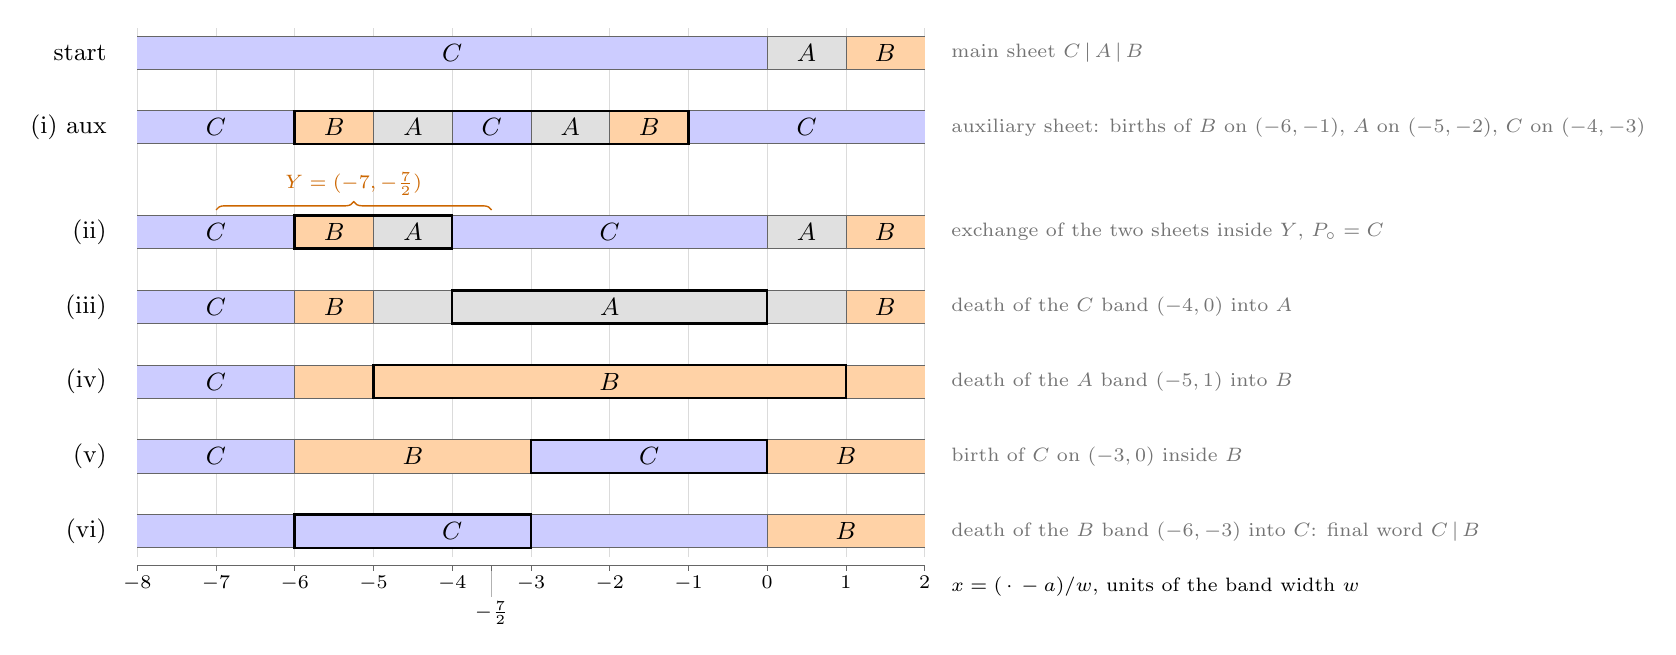
\begin{tikzpicture}[x=1cm, y=1cm, line width=0.3pt,
    lab/.style={font=\small, inner sep=1pt},
    name/.style={font=\scriptsize, text=black!55, inner sep=1pt},
    coord/.style={font=\scriptsize, inner sep=1pt},
    edge/.style={draw=black!60, line width=0.3pt},
    C/.style={fill=blue!20},
    A/.style={fill=black!12},
    B/.style={fill=orange!35},
    moved/.style={draw=black, line width=0.9pt},
    brace/.style={decorate, decoration={brace, amplitude=3pt}}]
  \def\xa{-8}\def\xb{2}\def\h{0.42}\def\dy{0.95}\def\yY{0.38}  % extra room above row (ii) for the bracket Y
  \newcommand\seg[3]{\fill[#3] (#1, 0) rectangle (#2, \h);
    \node[lab] at ({0.5*(#1+#2)}, 0.5*\h) {\(#3\)};}
  \newcommand\barframe[1]{\draw[edge] (\xa, 0) -- (\xb, 0) (\xa, \h) -- (\xb, \h);
    \foreach \xi in {#1} {\draw[edge] (\xi, 0) -- (\xi, \h);}}
  \newcommand\moved[2]{\draw[moved] (#1, 0) rectangle (#2, \h);}
  \foreach \xi in {-8,...,2} {\draw[black!14] (\xi, {-6*\dy-\yY-0.12}) -- (\xi, \h+0.1);}
  \begin{scope}[yshift=0cm]
    \node[lab, anchor=east] at (\xa-0.35, 0.5*\h) {start};
    \seg{\xa}{0}{C} \seg{0}{1}{A} \seg{1}{\xb}{B}
    \barframe{0,1}
    \node[name, anchor=west] at (\xb+0.3, 0.5*\h) {main sheet \(C\,|\,A\,|\,B\)};
  \end{scope}
  \begin{scope}[yshift=-\dy cm]
    \node[lab, anchor=east] at (\xa-0.35, 0.5*\h) {(i) aux};
    \seg{\xa}{-6}{C} \seg{-6}{-5}{B} \seg{-5}{-4}{A} \seg{-4}{-3}{C}
    \seg{-3}{-2}{A} \seg{-2}{-1}{B} \seg{-1}{\xb}{C}
    \barframe{-6,-5,-4,-3,-2,-1}
    \moved{-6}{-1}
    \node[name, anchor=west] at (\xb+0.3, 0.5*\h)
      {auxiliary sheet: births of \(B\) on \((-6,-1)\), \(A\) on \((-5,-2)\), \(C\) on \((-4,-3)\)};
  \end{scope}
  \begin{scope}[yshift={(-2*\dy-\yY)*1cm}]
    \node[lab, anchor=east] at (\xa-0.35, 0.5*\h) {(ii)};
    \seg{\xa}{-6}{C} \seg{-6}{-5}{B} \seg{-5}{-4}{A} \seg{-4}{0}{C}
    \seg{0}{1}{A} \seg{1}{\xb}{B}
    \barframe{-6,-5,-4,0,1}
    \moved{-6}{-4}
    \draw[brace, orange!80!black, line width=0.5pt] (-7, \h+0.07) -- (-3.5, \h+0.07)
      node[coord, midway, above=4pt, text=orange!80!black] {\(Y=(-7,-\tfrac72)\)};
    \node[name, anchor=west] at (\xb+0.3, 0.5*\h) {exchange of the two sheets inside \(Y\), \(P_\circ=C\)};
  \end{scope}
  \begin{scope}[yshift={(-3*\dy-\yY)*1cm}]
    \node[lab, anchor=east] at (\xa-0.35, 0.5*\h) {(iii)};
    \seg{\xa}{-6}{C} \seg{-6}{-5}{B} \seg{-5}{1}{A} \seg{1}{\xb}{B}
    \barframe{-6,-5,1}
    \moved{-4}{0}
    \node[name, anchor=west] at (\xb+0.3, 0.5*\h) {death of the \(C\) band \((-4,0)\) into \(A\)};
  \end{scope}
  \begin{scope}[yshift={(-4*\dy-\yY)*1cm}]
    \node[lab, anchor=east] at (\xa-0.35, 0.5*\h) {(iv)};
    \seg{\xa}{-6}{C} \seg{-6}{\xb}{B}
    \barframe{-6}
    \moved{-5}{1}
    \node[name, anchor=west] at (\xb+0.3, 0.5*\h) {death of the \(A\) band \((-5,1)\) into \(B\)};
  \end{scope}
  \begin{scope}[yshift={(-5*\dy-\yY)*1cm}]
    \node[lab, anchor=east] at (\xa-0.35, 0.5*\h) {(v)};
    \seg{\xa}{-6}{C} \seg{-6}{-3}{B} \seg{-3}{0}{C} \seg{0}{\xb}{B}
    \barframe{-6,-3,0}
    \moved{-3}{0}
    \node[name, anchor=west] at (\xb+0.3, 0.5*\h) {birth of \(C\) on \((-3,0)\) inside \(B\)};
  \end{scope}
  \begin{scope}[yshift={(-6*\dy-\yY)*1cm}]
    \node[lab, anchor=east] at (\xa-0.35, 0.5*\h) {(vi)};
    \seg{\xa}{0}{C} \seg{0}{\xb}{B}
    \barframe{0}
    \moved{-6}{-3}
    \node[name, anchor=west] at (\xb+0.3, 0.5*\h) {death of the \(B\) band \((-6,-3)\) into \(C\): final word \(C\,|\,B\)};
  \end{scope}
  \begin{scope}[yshift={(-6*\dy-\yY)*1cm}]
    \draw[black!60] (\xa, -0.22) -- (\xb, -0.22);
    \foreach \xi in {-8,...,2} {
      \draw[black!60] (\xi, -0.22) -- (\xi, -0.3);
      \node[coord, anchor=north] at (\xi, -0.32) {\(\xi\)};}
    \draw[black!60] (-3.5, -0.22) -- (-3.5, -0.3);
    \draw[black!30] (-3.5, -0.3) -- (-3.5, -0.62);
    \node[coord, anchor=north] at (-3.5, -0.64) {\(-\tfrac72\)};
    \node[coord, anchor=west] at (\xb+0.3, -0.5) {\(x=(\,\cdot\,-a)/w\), units of the band width \(w\)};
  \end{scope}
\end{tikzpicture}

\end{adjustbox}
\caption{The band dissolution in units of the band width: the auxiliary word after its three births (the heavier outline marks their union), the exchange window $Y$, and the sequence of deaths and births that leaves the band to $B$ with the interface back at zero.}\label{fig:band-words}
\end{figure*}

\begin{lemma}[The band dissolution is a bounded change]\label{lem:band}
For all sufficiently large $L$, each of the eight moves (seven births or
deaths and one exchange) in Construction~\ref{con:band} satisfies the information hypothesis of
Lemma~\ref{lem:birth} or Lemma~\ref{lem:exchange} with exponent $2p=24$,
so that the construction is a bounded change on the parties $A,B,C$ with
total reference-vector error at most $12L^{-12}$. Afterwards, the main
sheet reads $C\,|\,B$ with the interface at $x=0$, and all other ownership
is unchanged.
\end{lemma}
\begin{proof}
We verify the separation hypothesis for each move; all distances are measured in units of $w\ge D_{24}\log L$, and
every modified region is a single interval, so Lemma~\ref{lem:logsep} applies whenever the scaled separation is at least $1$.
(i) The first auxiliary birth has $E=\varnothing$ and requires no
information bound. The second modifies $(-5,-2)$ inside the
$B$ band $(-6,-1)$, so the non-$B$ region $E$ lies at distance $1$. The
third modifies $(-4,-3)$ inside the $A$ band $(-5,-2)$, again at distance $1$ from $E$. The
auxiliary word is now $C|B|A|C|A|B|C$ with interfaces at $-6,-5,-4,-3,-2,-1$.
(ii) The main sheet is owned by $C$ on $x<0$, while the auxiliary sheet is owned by $C$ on
$x<-6$, $(-4,-3)$, and $x>-1$. Hence $T=Z\cap Y=(-6,-4)$ (owned by $B$ and
$A$ on the auxiliary sheet) and $E=Z\setminus Y=(-3,-1)\cup[0,\infty)$, together with $x\le-8$ if $C$
owns no sites beyond $x=-8$; thus $\dist(T,E)\ge 1$.
After the exchange, the main sheet inside $Y$ inherits the auxiliary
assignment, yielding $C|B|A|C|A|B$ with interfaces at $-6,-5,-4,0,1$, while the auxiliary sheet
is owned by $C$ throughout $Y$.
(iii) On the main sheet, the $C$ band $(-4,0)$ is flanked by $A$ on $(-5,-4)\cup(0,1)$,
so the non-$A$ sites after the death lie in $x\le-5$ and $x\ge1$, at
distance $1$. Next, the $A$ band $(-5,1)$ is flanked by $B$ on
$(-6,-5)\cup(1,2)$, so the non-$B$ sites after the death lie in $x\le-6$ and $x\ge2$,
at distance $1$. The birth of $C$ on $(-3,0)$ inside $B$ has non-$B$ sites
at distance at least $2$. Finally, the death of $(-6,-3)$ into $C$ has non-$C$ sites in
$x\ge0$ at distance $3$ and, if $C$ owns nothing beyond $x=-8$, in
$x\le-8$ at distance $2$. Each of the seven births or deaths incurs error at most $L^{-12}$ and the exchange incurs at most
$4L^{-12}$, giving total error at most $11L^{-12}\le 12L^{-12}$.
\end{proof}

\begin{figure*}[t]
\centering
\begin{adjustbox}{max width=\linewidth}
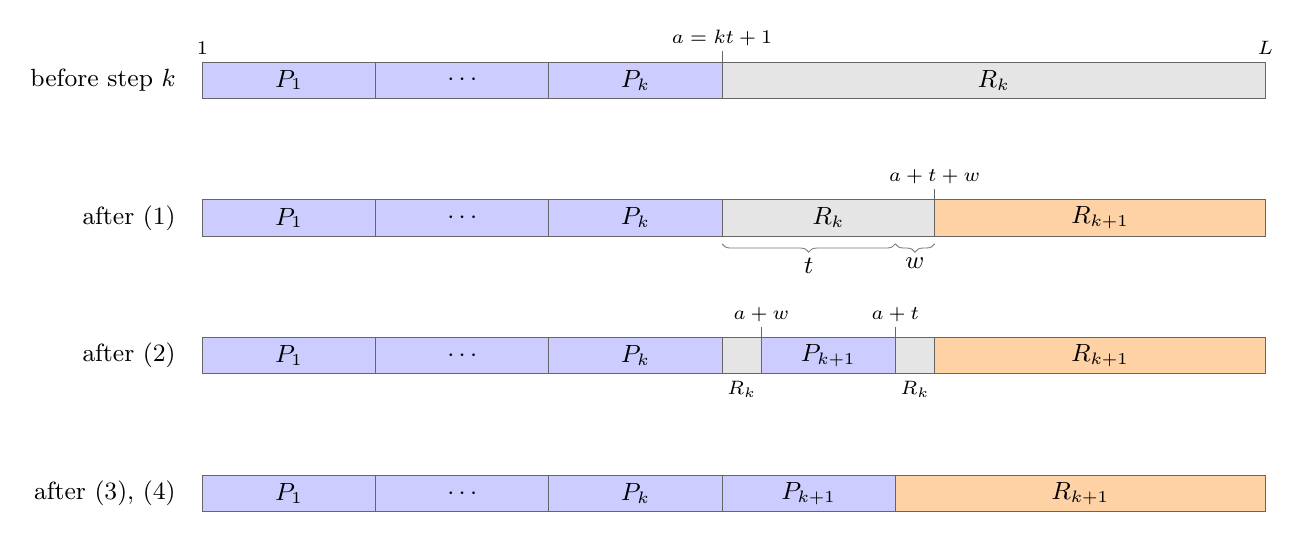
\begin{tikzpicture}[x=1cm, y=1cm, line width=0.3pt,
    lab/.style={font=\small, inner sep=1pt},
    name/.style={font=\scriptsize, text=black!55, inner sep=1pt},
    coord/.style={font=\scriptsize, inner sep=1pt},
    seg/.style={draw=black!60, line width=0.3pt},
    P/.style={seg, fill=blue!20},
    Rk/.style={seg, fill=black!10},
    Rn/.style={seg, fill=orange!35},
    brace/.style={decorate, decoration={brace, mirror, amplitude=3pt}}]
  \def\t{2.2}\def\w{0.5}\def\L{13.5}
  \def\a{6.6}      % a = k t + 1, the first site of block k+1 (3 t)
  \def\h{0.46}     % bar height
  \def\dy{1.75}    % row spacing
  \begin{scope}[yshift=0cm]
    \node[lab, anchor=east] at (-0.3, 0.5*\h) {before step \(k\)};
    \fill[P] (0, 0) rectangle (\t, \h);
    \fill[P] (\t, 0) rectangle (2*\t, \h);
    \fill[P] (2*\t, 0) rectangle (\a, \h);
    \fill[Rk] (\a, 0) rectangle (\L, \h);
    \node[lab] at (0.5*\t, 0.5*\h) {\(P_1\)};
    \node[lab] at (1.5*\t, 0.5*\h) {\(\cdots\)};
    \node[lab] at (2.5*\t, 0.5*\h) {\(P_k\)};
    \node[lab] at ({0.5*(\a+\L)}, 0.5*\h) {\(R_k\)};
    \node[coord, anchor=south] at (0, \h+0.05) {\(1\)};
    \node[coord, anchor=south] at (\L, \h+0.05) {\(L\)};
    \draw[black!60] (\a, \h) -- (\a, \h+0.14);
    \node[coord, anchor=south] at (\a, \h+0.16) {\(a=kt+1\)};
  \end{scope}
  \begin{scope}[yshift=-\dy cm]
    \node[lab, anchor=east] at (-0.3, 0.5*\h) {after (1)};
    \fill[P] (0, 0) rectangle (\t, \h);
    \fill[P] (\t, 0) rectangle (2*\t, \h);
    \fill[P] (2*\t, 0) rectangle (\a, \h);
    \fill[Rk] (\a, 0) rectangle (\a+\t+\w, \h);
    \fill[Rn] (\a+\t+\w, 0) rectangle (\L, \h);
    \node[lab] at (0.5*\t, 0.5*\h) {\(P_1\)};
    \node[lab] at (1.5*\t, 0.5*\h) {\(\cdots\)};
    \node[lab] at (2.5*\t, 0.5*\h) {\(P_k\)};
    \node[lab] at ({\a+0.5*(\t+\w)}, 0.5*\h) {\(R_k\)};
    \node[lab] at ({0.5*(\a+\t+\w+\L)}, 0.5*\h) {\(R_{k+1}\)};
    \draw[black!60] (\a+\t+\w, \h) -- (\a+\t+\w, \h+0.14);
    \node[coord, anchor=south] at (\a+\t+\w, \h+0.16) {\(a+t+w\)};
    \draw[brace, black!55] (\a, -0.1) -- (\a+\t, -0.1)
      node[lab, midway, below=4pt, text=black] {\(t\)};
    \draw[brace, black!55] (\a+\t, -0.1) -- (\a+\t+\w, -0.1)
      node[lab, midway, below=4pt, text=black] {\(w\)};
  \end{scope}
  \begin{scope}[yshift=-2*\dy cm]
    \node[lab, anchor=east] at (-0.3, 0.5*\h) {after (2)};
    \fill[P] (0, 0) rectangle (\t, \h);
    \fill[P] (\t, 0) rectangle (2*\t, \h);
    \fill[P] (2*\t, 0) rectangle (\a, \h);
    \fill[Rk] (\a, 0) rectangle (\a+\w, \h);
    \fill[P] (\a+\w, 0) rectangle (\a+\t, \h);
    \fill[Rk] (\a+\t, 0) rectangle (\a+\t+\w, \h);
    \fill[Rn] (\a+\t+\w, 0) rectangle (\L, \h);
    \node[lab] at (0.5*\t, 0.5*\h) {\(P_1\)};
    \node[lab] at (1.5*\t, 0.5*\h) {\(\cdots\)};
    \node[lab] at (2.5*\t, 0.5*\h) {\(P_k\)};
    \node[lab] at ({\a+0.5*(\t+\w)}, 0.5*\h) {\(P_{k+1}\)};
    \node[lab] at ({0.5*(\a+\t+\w+\L)}, 0.5*\h) {\(R_{k+1}\)};
    \node[coord, anchor=north] at (\a+0.5*\w, -0.06) {\(R_k\)};
    \node[coord, anchor=north] at (\a+\t+0.5*\w, -0.06) {\(R_k\)};
    \draw[black!60] (\a+\w, \h) -- (\a+\w, \h+0.14);
    \node[coord, anchor=south] at (\a+\w, \h+0.16) {\(a+w\)};
    \draw[black!60] (\a+\t, \h) -- (\a+\t, \h+0.14);
    \node[coord, anchor=south] at (\a+\t, \h+0.16) {\(a+t\)};
  \end{scope}
  \begin{scope}[yshift=-3*\dy cm]
    \node[lab, anchor=east] at (-0.3, 0.5*\h) {after (3), (4)};
    \fill[P] (0, 0) rectangle (\t, \h);
    \fill[P] (\t, 0) rectangle (2*\t, \h);
    \fill[P] (2*\t, 0) rectangle (\a, \h);
    \fill[P] (\a, 0) rectangle (\a+\t, \h);
    \fill[Rn] (\a+\t, 0) rectangle (\L, \h);
    \node[lab] at (0.5*\t, 0.5*\h) {\(P_1\)};
    \node[lab] at (1.5*\t, 0.5*\h) {\(\cdots\)};
    \node[lab] at (2.5*\t, 0.5*\h) {\(P_k\)};
    \node[lab] at (\a+0.5*\t, 0.5*\h) {\(P_{k+1}\)};
    \node[lab] at ({0.5*(\a+\t+\L)}, 0.5*\h) {\(R_{k+1}\)};
  \end{scope}
\end{tikzpicture}

\end{adjustbox}
\caption{One step of the sweep (for $k\ge1$): the word before the step, after the birth of $R_{k+1}$, after the birth of $P_{k+1}$, and after the two bands of $R_k$ have been dissolved.}\label{fig:sweep-step}
\end{figure*}

\begin{construction}[The sweep]\label{con:sweep}
Initially, a single party $R_0$ holds the entire sheet. For $k=0,1,\dots,k_*-1$, let
$a=kt+1$ be the first site of block $B_{k+1}$, and starting from the ownership word $P_1|\cdots|P_k|R_k$:
\begin{enumerate}[leftmargin=2em]
\item[(1)] Birth $R_{k+1}$ on $[a+t+w,L]$ inside $R_k$.
\item[(2)] Birth $P_{k+1}$ on $[a+w,a+t-1]$ inside $R_k$.
\item[(3)] Dissolve the band $[a,a+w-1]$ (owned by $R_k$) between $C=P_k$
and $B=P_{k+1}$ using Construction~\ref{con:band}; if $k=0$, let the band die directly
into $P_1$.
\item[(4)] Dissolve the band $[a+t,a+t+w-1]$ (owned by $R_k$) between
$C=P_{k+1}$ and $B=R_{k+1}$ using Construction~\ref{con:band}.
\end{enumerate}
After step $k_*-1$, set $P_{k_*+1}=R_{k_*}$, which owns the final block $B_{k_*+1}$.
\end{construction}

\begin{proposition}[Properties of the sweep]\label{prop:sweep}
For all sufficiently large $L$, Construction~\ref{con:sweep} defines a
distributed construction with the following properties:
\begin{enumerate}[leftmargin=2em]
\item There are $2k_*+1\le 2L$ parties. The initial state is a product state across
parties: $R_0$ holds $\Om$ on the main sheet, and every auxiliary copy of $\Om$ is initialised
privately at the party $C$ of the corresponding band dissolution.
\item There are at most $20k_*\le 2L$ non-private gates. Each involves at
most three parties and is admissible with one shared vector or covector
per monomial. Each party participates in at most $40$ non-private gates
over its lifetime.
\item The final vector $\Psi$ satisfies $\norm\Psi\le1$ and
$\norm{\Psi-\Om\otimes\Xi}\le 26\,L^{-11}$, where $\Xi$ is the tensor
product of the retired auxiliary copies of $\Om$ in their final registers
and $\norm\Xi=1$. At the end of the sweep, party $P_i$ owns precisely the raw registers
of block $B_i$, of dimension $q^{\abs{B_i}}\le q^{4t}=L^{O(1)}$, and no other
party owns any raw register.
\end{enumerate}
\end{proposition}
\begin{proof}
At the start of step $k$, the ownership word is $P_1|\cdots|P_k|R_k$, with $R_k$ owning
$[a,L]$ for $a=kt+1$. Move (1) modifies $[a+t+w,L]$ with non-$R_k$ region
$E=[1,a-1]$ at distance $t+w$; move (2) modifies $[a+w,a+t-1]$ with non-$R_k$ region
$E=[1,a-1]\cup[a+t+w,L]$ at distance $w$. Both moves are valid births by
Lemma~\ref{lem:birth} and Lemma~\ref{lem:logsep}. Afterwards, $R_k$ owns
only the two bands $[a,a+w-1]$ and $[a+t,a+t+w-1]$. In (3), $C=P_k$ owns
block $B_k$ of length $t=20w\ge8w$ to the left of $a$, and $B=P_{k+1}$ owns
$[a+w,a+t-1]$ of length $19w\ge2w$, so Lemma~\ref{lem:band} applies
(when $k=0$, the direct death of $[1,w]$ into $P_1$ has non-$P_1$ region $E=[t+1,L]$ at distance
$t-w\ge w$). In (4), $C=P_{k+1}$ owns $[a+w,a+t-1]$ of length $19w\ge8w$ and
$B=R_{k+1}$ owns $[a+t+w,L]$ of length at least $3t-w\ge2w$, so Lemma~\ref{lem:band} again applies. Step $k$ concludes with
the word $P_1|\cdots|P_{k+1}|R_{k+1}$. The distinct parties are $R_0,\dots,R_{k_*}$
and $P_1,\dots,P_{k_*}$, with $P_{k_*+1}=R_{k_*}$. Each step uses at most $2+2\cdot8=18\le20$ moves, giving at most $20k_*$ moves in total, and the final
block has length in $[3t,4t)$.

For participation counts, $R_k$ participates only in step $k-1$ (as the newborn party in (1)
and as $B$ in (4)) and in step $k$ (as $P_\circ$ in (1) and (2), and as $A$ in (3) and
(4)); similarly, $P_k$ participates only in step $k-1$ (born in (2), acting as $B$ in (3) and $C$ in (4))
and in step $k$ (acting as $C$ in (3)). Because each band dissolution consists of seven births or deaths and one
private exchange, no party participates in more than $2\cdot(2+2\cdot8)=36\le40$ gates.
Every birth or death is a single two-party gate with one shared
vector or covector, while every exchange is purely private.

For the error bound, each move maps the current state vector to within the stated
error of the updated reference vector, which is the tensor product of $\Om$
on the main sheet and $\Om$ on each active or retired auxiliary sheet in canonical
coordinates (Lemmas~\ref{lem:birth} and~\ref{lem:exchange}; retired auxiliary sheets
remain unit-norm spectators). Telescoping the product of contractions bounds
the total error by the sum of the per-move errors: two births and
two band dissolutions per step contribute at most $(2+2\cdot12)L^{-12}$, so the cumulative error over $k_*$ steps
is at most $26k_*L^{-12}\le 26L^{-11}$. Since the initial vector has unit norm and every gate is a
contraction, $\norm\Psi\le1$.
\end{proof}

\begin{figure*}[t]
\centering
\begin{adjustbox}{max width=\linewidth}
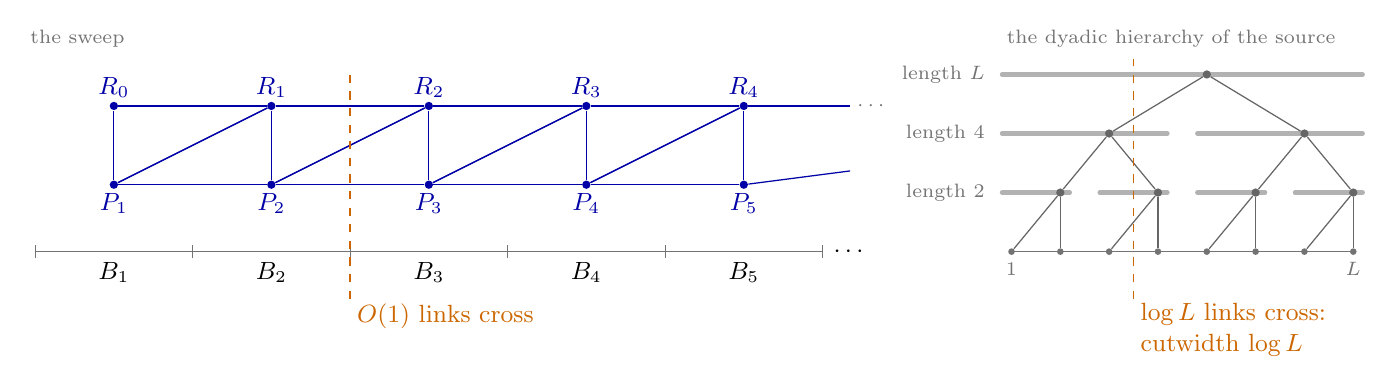
\begin{tikzpicture}[x=1cm, y=1cm, line width=0.3pt,
    lab/.style={font=\small, inner sep=1pt},
    annot/.style={font=\scriptsize, text=black!55, inner sep=1pt},
    party/.style={circle, fill=blue!65!black, inner sep=0pt, minimum size=3pt},
    link/.style={draw=blue!65!black, line width=0.45pt},
    site/.style={circle, fill=black!55, inner sep=0pt, minimum size=2.4pt},
    dnode/.style={circle, fill=black!60, inner sep=0pt, minimum size=3pt},
    dlink/.style={draw=black!60, line width=0.45pt},
    bar/.style={draw=black!30, line width=1.6pt, line cap=round},
    cut/.style={dashed, color=orange!80!black, line width=0.5pt}]
  \def\b{2.0}\def\yP{0.85}\def\yR{1.85}
  \node[annot, anchor=south west] at (-0.1, 2.55) {the sweep};
  \draw[black!55] (0, 0) -- (5*\b, 0);
  \foreach \i in {0,...,5} { \draw[black!55] (\i*\b, 0.08) -- (\i*\b, -0.08); }
  \foreach \i in {1,...,5} {
    \node[lab, anchor=north] at ({(\i-0.5)*\b}, -0.1) {\(B_{\i}\)};
  }
  \node[lab, anchor=west] at (5*\b + 0.1, 0) {\(\cdots\)};
  \foreach \i in {1,...,5} {
    \node[party] (P\i) at ({(\i-0.5)*\b}, \yP) {};
    \node[lab, anchor=north, text=blue!65!black] at ({(\i-0.5)*\b}, \yP-0.07) {\(P_{\i}\)};
  }
  \foreach \k in {0,...,4} {
    \pgfmathtruncatemacro{\j}{\k+1}
    \node[party] (R\k) at ({(\j-0.5)*\b}, \yR) {};
    \node[lab, anchor=south, text=blue!65!black] at ({(\j-0.5)*\b}, \yR+0.07) {\(R_{\k}\)};
  }
  \draw[link] (P1) -- (R0);
  \draw[link] (R0) -- (R1);
  \draw[link] (P1) -- (R1);
  \foreach \k in {1,...,4} {
    \pgfmathtruncatemacro{\j}{\k+1}
    \draw[link] (P\k) -- (R\k);
    \draw[link] (P\j) -- (R\k);
    \draw[link] (P\k) -- (P\j);
    \ifnum\k<4
      \draw[link] (R\k) -- (R\j);
      \draw[link] (P\j) -- (R\j);
    \fi
  }
  \draw[link] (R4) -- (5*\b + 0.35, \yR);
  \draw[link] (P5) -- (5*\b + 0.35, {\yP + 0.5*(\yR-\yP)*0.35/\b*2});
  \node[annot, anchor=west] at (5*\b + 0.4, \yR) {\(\cdots\)};
  \draw[cut] (2*\b, -0.6) -- (2*\b, 2.3);
  \node[lab, anchor=north west, text=orange!80!black] at (2*\b + 0.05, -0.62) {\(O(1)\) links cross};
  \begin{scope}[xshift=12.4cm]
    \def\s{0.62}\def\h{0.75}
    \node[annot, anchor=south west] at (-0.1, 2.55) {the dyadic hierarchy of the source};
    \draw[black!55] (0, 0) -- (7*\s, 0);
    \foreach \i in {1,...,8} {
      \node[site] (S\i) at ({(\i-1)*\s}, 0) {};
    }
    \node[annot, anchor=north] at (0, -0.1) {\(1\)};
    \node[annot, anchor=north] at (7*\s, -0.1) {\(L\)};
    \foreach \a/\c/\p in {1/2/2, 3/4/4, 5/6/6, 7/8/8} {
      \draw[bar] ({(\a-1)*\s - 0.12}, \h) -- ({(\c-1)*\s + 0.12}, \h);
      \node[dnode] (D\a\c) at ({(\p-1)*\s}, \h) {};
      \draw[dlink] (D\a\c) -- (S\a);
      \draw[dlink] (D\a\c) -- (S\c);
    }
    \foreach \a/\m/\n/\c/\p in {1/2/3/4/3, 5/6/7/8/7} {
      \draw[bar] ({(\a-1)*\s - 0.12}, 2*\h) -- ({(\c-1)*\s + 0.12}, 2*\h);
      \node[dnode] (D\a\c) at ({(\p-1)*\s}, 2*\h) {};
      \draw[dlink] (D\a\c) -- (D\a\m);
      \draw[dlink] (D\a\c) -- (D\n\c);
    }
    \draw[bar] (-0.12, 3*\h) -- (7*\s + 0.12, 3*\h);
    \node[dnode] (D18) at (4*\s, 3*\h) {};
    \draw[dlink] (D18) -- (D14);
    \draw[dlink] (D18) -- (D58);
    \node[annot, anchor=east] at (-0.3, \h) {length \(2\)};
    \node[annot, anchor=east] at (-0.3, 2*\h) {length \(4\)};
    \node[annot, anchor=east] at (-0.3, 3*\h) {length \(L\)};
    \draw[cut] (2.5*\s, -0.6) -- (2.5*\s, 2.45);
    \node[lab, anchor=north west, text=orange!80!black, align=left] at (2.5*\s + 0.05, -0.62)
      {\(\log L\) links cross:\\ cutwidth \(\log L\)};
  \end{scope}
\end{tikzpicture}

\end{adjustbox}
\caption{Left: the party graph of the sweep placed on the chain; a bounded number of links cross any bond. Right: a dyadic hierarchy drawn on a line, where every scale contributes a link across the middle bond.}\label{fig:party-graph}
\end{figure*}

\begin{remark}[Why small-patch rewrites are unneeded]
In two dimensions \cite[Section~4]{PP}, squares of side length below $K_0\log L$
must be repainted by ``small-patch rewrites'' using finite-rank cylinder
projections of polynomial rank. In one dimension, the final owners $P_i$ hold
blocks of $O(\log L)$ consecutive sites whose Hilbert-space dimension
$q^{\abs{B_i}}=q^{O(\log L)}$ is already polynomial in $L$, and the compression
theorem of Section~\ref{sec:compression} accepts polynomial-dimensional physical
outputs directly. Factoring each block tensor into single-site matrix-product
tensors is then a routine singular value decomposition (Section~\ref{sec:routing}).
This is the second reason why the adaptive patch constraints of \cite{PP} are
unneeded on a chain.
\end{remark}

\section{Compression and column extraction}\label{sec:compression}

\begin{inwords}
The sweep protocol is a sequence of linear contractions followed by a partial
trace over all registers except the physical block outputs. Its non-private
gates still rely on shared bipartite vectors of enormous dimension (such as
purifications of half-chain marginals). To compress these virtual links to
polynomial dimension, the density-compression theorem replaces each shared
source operator $\ket\eta\bra{\tilde\eta}$ in the density calculation
$\rho=\Tr_{\mathrm{private}}\ket\Psi\bra\Psi$ with the sample average of $k$
independent random product operators $U_j\otimes V_j$ built from its Schmidt
decomposition and standard complex Gaussian coefficients. For a polynomial
sample size $k$, the physical output density changes by at most $L^{-p}$ in
trace norm. Expanding the error according to the subset of slots where a
centred correction $\widehat X-X$ acts, each corrected slot involves only its
two endpoint parties, and bounded participation ensures that only a bounded
number of gates per corrected slot must be expanded into monomials; a
Gaussian second-moment computation with Schatten--Hölder then shows that a
term with $s$ corrections has expected trace norm at most $k^{-s/2}$ times a
fixed polynomial per correction. Because this estimate depends only on the
trace-one Schmidt probability weights and the combinatorial participation
bounds, it is completely independent of the private Hilbert-space dimensions
and of the Schmidt ranks of the shared states. Fixing a deterministic
realisation produces an operator tensor network $\sigma$ with one node per
party and polynomial-dimensional links between parties that shared a gate.
Extracting a single product-basis column $\sigma\ket z$ then converts
$\sigma$ into a ket tensor network with the same virtual links, which
approximates the ground vector after normalisation. The theorem and its
proof are not geometric and carry over without change; we restate the
theorem in the form used here and sketch the estimate.
\end{inwords}

\precisely
\begin{theorem}[Density compression, {\cite[Theorem~5.2]{PP}}]\label{thm:compression}
Consider a family of distributed constructions indexed by $L\ge2$ such
that: the numbers of parties and gates are uniformly polynomial; the
initial vector is a product of normalised private vectors; every gate is
a contraction; each non-private gate involves at most $b$ parties and each
party participates in at most $b$ non-private gates; each non-private gate
is admissible with uniformly polynomial bounds; and the intended physical
output of each party has uniformly polynomial dimension, everything else
being traced out. Let $\rho$ be the physical output density (positive,
trace at most one). For every fixed $p>0$ there is an operator tensor
network $\sigma$ with one node per party, a bounded number of links at
each node, each link joining two parties that participate in a common
non-private gate, uniformly polynomial link dimensions, and
\[
 \norm{\sigma-\rho}_1\le L^{-p}.
\]
The constants depend only on $p$, $b$, and the uniform polynomial bounds,
not on private dimensions or on the Schmidt ranks of shared vectors.
\end{theorem}
\begin{proof}[Sketch]
First eliminate shared covectors: a covector $\bra\eta$ on a pair of
registers is replaced by appending $m-1$ copies of $\eta$ and averaging over the
$m$ cyclic permutations of the $m$ pair registers, forming a contraction $T_m$ with
$\norm{T_m-\ket\eta^{\otimes m}\bra\eta}=m^{-1/2}$. Attaching a common fixed
garbage vector in every branch approximates a gate with $K$ monomials, each containing at
most $r$ covectors, to within operator-norm error
$rm^{-1/2}\sum\abs{c_\xi}$ by a gate with $Km^r$ monomials using shared
vectors only. Choosing $m$ polynomially large makes this error at most
$\epsilon/(8M)$ per gate, where $M$ is the number of non-private gates.

Next, in the density calculation, each source operator $X=\ket\eta\bra{\tilde\eta}$
with Schmidt decompositions $(\lambda_a,u_a,v_a)$ and $(\mu_c,\tilde u_c,\tilde v_c)$
is replaced by $\widehat X=\frac1k\sum_{j=1}^kU_j\otimes V_j$, where
$U_j=\sum_{a,c}(\lambda_a\mu_c)^{1/4}g^{(j)}_{ac}\ket{u_a}\bra{\tilde u_c}$ and
$V_j=\sum_{b,d}(\lambda_b\mu_d)^{1/4}\overline{g^{(j)}_{bd}}\ket{v_b}\bra{\tilde v_d}$
for independent standard complex Gaussians $g^{(j)}_{ac}$. Then
$\E\widehat X=X$, and by the Gaussian pairing formula the centred coefficients of $\Delta=\widehat X-X$ have
diagonal covariance $k^{-1}\sqrt{\lambda_a\lambda_b\mu_c\mu_d}$. Expanding the product over all $N$ source
slots gives $\widehat\rho-\rho'=\sum_{\varnothing\ne S}F_S$, where $S$ indexes
the slots carrying a correction $\Delta$. For $\abs S=s$, the corrected slots touch
at most $2s$ endpoint parties, which participate in at most $2bs$ gates; expand only
those gates into monomials and fix the physical basis entries at those
parties, at a total weighted cost of at most $Q(L)^s$ for a fixed polynomial $Q$.
For each fixed choice, the network factors into an affected side
(holding the corrected endpoints as free inputs) and an exterior side, connected
only by the exact shared vectors crossing between them, with Schmidt
probability matrices $\tau$ and $\tilde\tau$. The affected contractions form a
block operator $O$ of norm at most one, the corrected coefficients $z_{il}$
have covariance $k^{-s}\sqrt{p_i\tilde p_l}\,\delta\delta$, and the operator fed into the exterior
is $Z=\sum_{il}z_{il}\tau^{1/2}O_{li}^{\mathsf T}\tilde\tau^{1/2}$.
Applying the Schatten--Hölder inequality with exponents $(4,2,4)$ and the trace-one weights $\tau,\tilde\tau$ gives
$\norm Z_1\le\norm{\sum_{il}z_{il}\tilde\tau^{1/4}O_{li}\tau^{1/4}}_2$, whose expected
square is $k^{-s}\norm{\widetilde R^{1/4}OR^{1/4}}_2^2\le k^{-s}$ with
$R=\mathrm{diag}(p_i)\otimes\tau$ and $\widetilde R=\mathrm{diag}(\tilde p_l)\otimes\tilde\tau$.
Because the exterior contractions and the physical matrix units are trace-norm contractions,
$\E\norm{F_S}_1\le Q(L)^sk^{-s/2}$ and hence
$\E\norm{\widehat\rho-\rho'}_1\le(1+Q(L)k^{-1/2})^N-1\le\epsilon/4$ for a
polynomial sample size $k$. Fixing a realisation of the Gaussian variables yields $\sigma$: the monomial
index of each gate is shared along a star linking its participating parties, and each
slot's sample index $j\in\{1,\dots,k\}$ is shared between its two endpoint parties, while all private
contractions, private state preparations, and final private traces are
absorbed into each party's local node tensor.
\end{proof}

\begin{figure}[t]
\centering
\begin{adjustbox}{max width=\linewidth}
\(\begin{tenkz}[size=l, rows={wire,wire}, cols=2, bonds=none]
  \tn[at=(1,1), skin=box, wide=2, ports={90@1:physical, 90@2:physical}]{\eta}
  \tn[at=(2,1), skin=box, wide=2, ports={270@1:physical, 270@2:physical}]{\tilde\eta^{\,\dagger}}
\end{tenkz}
=\mathbb E\,\frac1k
\begin{tenkz}[size=l, rows={wire}, cols=2, bonds=none]
  \tn[at=(1,1), name=u, skin=box, ports={0:virtual, 90:physical, 270:physical}]{U_j}
  \tn[at=(1,2), name=w, skin=box, ports={180:virtual, 90:physical, 270:physical}]{V_j}
  \tnbond[name=j]{u.0}{w.180}
\end{tenkz}\)

\end{adjustbox}
\caption{The random replacement of one pair source: the operator $\ket\eta\bra{\tilde\eta}$ equals the expectation of $\frac1k\sum_j U_j\otimes V_j$, the two factors joined by the sample index $j$.}\label{fig:source-sampling}
\end{figure}

\begin{lemma}[Column extraction, {\cite[Lemma~8.1]{PP}}]\label{lem:column}
Let $\Om$ be a unit vector on a finite tensor product and $\sigma$ an
operator with $\norm{\sigma-\ket\Om\bra\Om}_1\le\eta<1$. Then some
product-basis column $v=\sigma\ket z$ is nonzero and satisfies
$\min_\theta\norm{v/\norm v-\e^{i\theta}\Om}\le2\eta$. Fixing a column in an
operator tensor network leaves all virtual dimensions unchanged.
\end{lemma}
\begin{proof}
Let $E=\sigma-\ket\Om\bra\Om$ and $a_z=\langle\Om|z\rangle$. Since
$\sum_z\norm{E\ket z}^2=\norm E_2^2\le\eta^2$ and $\sum_z\abs{a_z}^2=1$,
there exists a product-basis label $z$ with $a_z\ne0$ and $\norm{E\ket z}\le\eta\abs{a_z}$. For this $z$,
the rescaled column $w=v/a_z$ satisfies $\norm{w-\Om}\le\eta$, so $w\ne0$ and
$\norm{w/\norm w-\Om}\le2\eta$. Fixing the bra index at every node contracts
only physical legs, leaving all virtual bond dimensions unchanged.
\end{proof}

\begin{figure}[t]
\centering
\begin{adjustbox}{max width=\linewidth}
\(\begin{tenkz}[size=l, rows={wire,wire}, cols=3, bonds=none]
  \tn[at=(1,1), name=a, skin=box, ports={0:virtual, 90:physical, 270:physical}]{\sigma}
  \tn[at=(1,2), name=b, skin=box, ports={180:virtual, 0:virtual, 90:physical, 270:physical}]{\sigma}
  \tn[at=(1,3), name=c, skin=box, ports={180:virtual, 90:physical, 270:physical}]{\sigma}
  \tn[at=(2,1), name=za, skin=tri, ports={90:physical}]{}
  \tn[at=(2,2), name=zb, skin=tri, ports={90:physical}]{}
  \tn[at=(2,3), name=zc, skin=tri, ports={90:physical}]{}
  \tnbond{a.0}{b.180} \tnbond{b.0}{c.180}
  \tnwire{a.270}{za.90} \tnwire{b.270}{zb.90} \tnwire{c.270}{zc.90}
\end{tenkz}
=
\begin{tenkz}[size=l, rows={wire}, cols=3, bonds=none]
  \tn[at=(1,1), name=a, skin=box, ports={0:virtual, 90:physical}]{v}
  \tn[at=(1,2), name=b, skin=box, ports={180:virtual, 0:virtual, 90:physical}]{v}
  \tn[at=(1,3), name=c, skin=box, ports={180:virtual, 90:physical}]{v}
  \tnbond{a.0}{b.180} \tnbond{b.0}{c.180}
\end{tenkz}\)

\end{adjustbox}
\caption{Column extraction: fixing the input legs of the operator chain by a product-basis covector gives a ket chain with the same bonds.}\label{fig:column}
\end{figure}

\section{Assembly on the chain}\label{sec:routing}

\begin{inwords}
We now apply density compression and column extraction to the sweep protocol
and route the resulting party network along the chain. The parties of the
sweep are the block owners $P_i$, whose physical outputs are the
$q^{\abs{B_i}}$-dimensional block registers, and the remainder parties $R_k$,
which have no physical outputs. Every link in the compressed party network
connects two parties that shared a non-private gate, and by construction
those parties belong to the same or adjacent sweep steps. Placing the node of
$R_k$ alongside block $B_{k+1}$ ensures that the chain cut between blocks
$B_i$ and $B_{i+1}$ is crossed only by links among the boundedly many parties
attached to the four nearest blocks. This bounded congestion implies that each
inter-block bond has dimension equal to a bounded product of polynomial link
dimensions. Column extraction first converts the compressed operator network
into a ket network on the blocks; sequential singular value decompositions
across the sites within each block then split each block tensor into
single-site tensors whose internal bond dimensions are at most
$q^{\abs{B_i}}$ times the inter-block bond dimension, which remains
polynomial in $L$. Chains shorter than the threshold $L_0$ are represented
exactly.
\end{inwords}

\precisely
\begin{proof}[Proof of Theorem~\ref{thm:B}]
Choose $L_0$ large enough for Proposition~\ref{prop:sweep} and for the
inequalities below to hold; for $2\le L<L_0$, every state vector on $\Lam$ admits an exact
matrix product state representation of bond dimension at most $q^{\lfloor L/2\rfloor}\le
q^{L_0/2}$, which is absorbed into the prefactor $C$. Assume henceforth that $L\ge L_0$.

By Proposition~\ref{prop:sweep}(3) and the inequality
$\norm{\ket u\bra u-\ket v\bra v}_1\le2\norm{u-v}$ for vectors of norm at
most one, the physical output density
$\rho=\Tr_{\mathrm{private}}\ket\Psi\bra\Psi$ satisfies
$\norm{\rho-\ket\Om\bra\Om}_1\le 52L^{-11}$. The sweep satisfies the
hypotheses of Theorem~\ref{thm:compression} with participation bound $b=40$ and physical
output dimensions at most $q^{4t}\le L^{80D_{24}\log q+1}$. Applying Theorem~\ref{thm:compression} with target
accuracy $L^{-5}$ yields an operator tensor network $\sigma$ on the party
graph with $\norm{\sigma-\ket\Om\bra\Om}_1\le L^{-5}+52L^{-11}\le2L^{-5}$,
bounded node degree, and link dimensions at most $C_1L^{r}$. By
Lemma~\ref{lem:column}, some product-basis column of $\sigma$ is a nonzero ket tensor network $v$ with the
same virtual links satisfying $\min_\theta\norm{v/\norm v-\e^{i\theta}\Om}\le4L^{-5}\le L^{-1}$.

\emph{Placement and routing.} Assign $P_i$ to block $B_i$ and $R_k$ to block $B_{k+1}$, and
contract the two party nodes assigned to each block into a single block node (links between them
cross no inter-block cut). By the proof of
Proposition~\ref{prop:sweep}, any two parties sharing a gate belong to
$\{P_k,P_{k+1},R_k,R_{k+1}\}$ for some step $k$, and are therefore assigned to the same
or adjacent blocks (our bound below accommodates blocks up to two apart). The cut between blocks $B_i$ and $B_{i+1}$ is thus
crossed only by links incident to parties assigned to blocks
$B_{i-1},\dots,B_{i+2}$. There are at most $8$ such parties, each of degree at most
$5\cdot40$ (at most two star links and three sample links per three-party
gate), so at most $\chi:=1600$ links cross any inter-block cut. Route each link along the chain
between its endpoint blocks and bundle the links crossing each inter-block cut into a single
bond index of dimension at most $(C_1L^r)^{\chi}$. The tensor at block $B_i$ is
then a linear map from its left and right inter-block bond spaces to the block's
physical Hilbert space $\cH_{B_i}$ of dimension at most $q^{4t}$. Writing
$B_i=\{x_1<\dots<x_n\}$, perform successive singular value decompositions
across the internal cuts $x_1|x_2\cdots x_n$, $x_1x_2|x_3\cdots x_n$, \dots,
treating the left and right inter-block bond indices as external legs attached to
$x_1$ and $x_n$. The resulting single-site tensors have internal
bond dimensions at most $\min\{q^{j}(C_1L^r)^\chi,\ q^{n-j}(C_1L^r)^\chi\}\le
q^{2t}(C_1L^r)^{\chi}$, while the inter-block bonds remain unchanged. Thus $v$ is a
matrix product state on $\Lam$ with open boundary conditions and bond
dimension at most $q^{2t}(C_1L^r)^\chi\le CL^{c}$, with exponent
$c=40D_{24}\log q+r\chi$.
\end{proof}

\begin{figure*}[t]
\centering
\begin{adjustbox}{max width=\linewidth}
\(\displaystyle \begin{tenkz}[size=l, rows={wire,wire}, cols=4, bonds=none]
    \tn[at=(2,1), skin=box, wide=4, name=b,
        ports={180:virtual:$(C_1L^r)^{\chi}$, 0:virtual:$(C_1L^r)^{\chi}$,
               90@1:physical, 90@2:physical, 90@3:physical, 90@4:physical}]{B_i}
    \tn[at=(1,1), skin=none, name=p1, ports={270:physical, 90:physical:$x_1$}]{}
    \tn[at=(1,2), skin=none, name=p2, ports={270:physical, 90:physical:$x_2$}]{}
    \tn[at=(1,3), skin=none, name=p3, ports={270:physical, 90:physical:$x_3$}]{}
    \tn[at=(1,4), skin=none, name=p4, ports={270:physical, 90:physical:$x_4$}]{}
    \tnwire{b.90@1}{p1.270} \tnwire{b.90@2}{p2.270}
    \tnwire{b.90@3}{p3.270} \tnwire{b.90@4}{p4.270}
  \end{tenkz}
  \;=\;
  \begin{tenkz}[size=l, rows={wire,wire}, cols=7, bonds=none]
    \tn[at=(2,1), name=a1, skin=box, ports={180:virtual:$(C_1L^r)^{\chi}$, 0:virtual, 90:physical}]{A^{[x_1]}}
    \tn[at=(2,3), name=a2, skin=box, ports={180:virtual, 0:virtual, 90:physical}]{A^{[x_2]}}
    \tn[at=(2,5), name=a3, skin=box, ports={180:virtual, 0:virtual, 90:physical}]{A^{[x_3]}}
    \tn[at=(2,7), name=a4, skin=box, ports={180:virtual, 0:virtual:$(C_1L^r)^{\chi}$, 90:physical}]{A^{[x_4]}}
    \tn[at=(1,1), skin=none, name=q1, ports={270:physical, 90:physical:$x_1$}]{}
    \tn[at=(1,3), skin=none, name=q2, ports={270:physical, 90:physical:$x_2$}]{}
    \tn[at=(1,5), skin=none, name=q3, ports={270:physical, 90:physical:$x_3$}]{}
    \tn[at=(1,7), skin=none, name=q4, ports={270:physical, 90:physical:$x_4$}]{}
    \tnwire{a1.90}{q1.270} \tnwire{a2.90}{q2.270} \tnwire{a3.90}{q3.270} \tnwire{a4.90}{q4.270}
    \tnbond[name=d1]{a1.0}{a2.180} \tnbond[name=d2]{a2.0}{a3.180} \tnbond[name=d3]{a3.0}{a4.180}
    \tnmark[form=label, label pos=90]{on d1 0.5}{$q^{2t}(C_1L^r)^{\chi}$}
    \tnmark[form=label, label pos=90]{on d2 0.5}{$q^{2t}(C_1L^r)^{\chi}$}
    \tnmark[form=label, label pos=90]{on d3 0.5}{$q^{2t}(C_1L^r)^{\chi}$}
  \end{tenkz}\)

\end{adjustbox}
\caption{A block tensor with its two block bonds and $t$ physical legs is split into $t$ site tensors by successive singular value decompositions; the new bonds are at most $q^{2t}$ times the block-bond dimension.}\label{fig:block-to-sites}
\end{figure*}

\begin{remark}[Order of constants]
Fix $q,R,J,\Delta$. Theorem~\ref{thm:A} determines the interval entropy bound $C_{\mathrm{int}}$;
Lemma~\ref{lem:reset} at exponent $p=24$ determines $C_{24}$, which fixes $D_{24}$ and the
block length $t=20w$; the party and gate counts together with the participation bound
$b=40$ are then fixed; Theorem~\ref{thm:compression} at accuracy $L^{-5}$
fixes the covector permutation count $m$, the Gaussian sample size $k$, and
the link-dimension exponent $r$; and the congestion bound $\chi=1600$ is an absolute numerical constant.
None of these constants depends on the specific Hamiltonian $H$ or on the chain length $L$. Over the full sweep, the protocol prepares
$O(L/\log L)$ auxiliary copies of $\Om$, all held privately.
\end{remark}

\section{Discussion}\label{sec:discussion}

\begin{inwords}
\emph{Comparison with earlier one-dimensional proofs.} Hastings' proof of the
one-dimensional area law \cite{Hastings2007} shows that the half-chain
marginal has an entanglement spectrum whose tail decays exponentially beyond
rank $\exp(O(1))$ by combining a Lieb--Robinson bound, a spectral filter
that approximately projects onto the ground state, and a bound on the
approximate factorisation of the filtered state. Arad, Kitaev, Landau, and Vazirani
\cite{AKLV} replace the time-evolution filter with an approximate
ground-state projector constructed from Chebyshev polynomials of controlled
Schmidt rank, which is then amplified by bootstrapping. By contrast, the
proof of Theorem~\ref{thm:A} in Part~\ref{part:arealaw} uses no real-time
dynamics at all: the spectral gap enters only to bound the overlap of a
variationally tilted or filtered vector with the ground vector, and the entanglement
entropy is extracted directly from operator norms via Hölder's inequality, a
three-lines interpolation, and the Araki--Lieb triangle
inequality, yielding a linear $O(J/\Delta)$ scaling in the inverse gap. For
Theorem~\ref{thm:B}, this note presents two distinct constructions of the
matrix product state: the direct two-line route of Section~\ref{sec:shortcut},
which combines the marginal tail bound (Lemma~\ref{lem:tail}) with the area
law (Theorem~\ref{thm:A}) and is likewise completely free of dynamics, and
the distributed protocol route of Part~\ref{part:mps}, which invokes a
Lieb--Robinson bound in a single place (the information reset,
Lemma~\ref{lem:reset}) but in a way that has no analogue in Hastings'
construction (a two-replica swap undone by a local unitary), and otherwise
relies solely on Uhlmann-type ownership moves, random Gaussian compression,
and product-basis column extraction.

\emph{Simplifications specific to one dimension.} Three geometric features of
the line simplify the two-dimensional arguments of \cite{AL,PP}, each used in
exactly one place. First, the shell around any interval is crossed by $O(1)$
interaction terms, so the buffered discount (Lemma~\ref{lem:buffer}) costs
a constant and needs only a constant-width buffer. Second, no three interval owners ever meet at a single point on
a line, eliminating trijunctions and the associated boundary encodings in the
ownership moves (Section~\ref{sec:moves}). Third, the chain can be swept
sequentially from left to right, giving a party graph of $O(1)$ cutwidth
rather than the $\log L$ cutwidth of a dyadic tree (Section~\ref{sec:sweep}).
Everything else in \cite{AL,PP} is either unchanged or disappears.

\emph{Why the two-dimensional obstructions are genuine.} None of these three
one-dimensional shortcuts extends back to two dimensions. In two dimensions,
the Araki--Lieb closure fails because the buffer surrounding a region is a
thin annulus whose own entanglement entropy is a priori unknown; a linear
sweep fails because repainting a two-dimensional region exposes a
one-dimensional boundary along which a third owner is adjacent, necessitating
the edge-band dissolutions and trijunction treatments of \cite{PP}; and sequential
Schmidt truncation across nested cuts does not produce a two-dimensional
tensor network on the lattice. The multiscale machinery of
\cite{AL,PP} is therefore dictated by genuine two-dimensional geometric and
topological obstructions that simply do not arise on a chain.
\end{inwords}

\begin{thebibliography}{9}
\bibitem{AL} OpenAI, \emph{A two-dimensional area law from a global spectral gap}, manuscript of September 24, 2026, \texttt{openai/math} revision \texttt{adc7f12}.
\bibitem{PP} OpenAI, \emph{Polynomial PEPS approximation of gapped square-grid ground states}, manuscript of September 24, 2026, \texttt{openai/math} revision \texttt{adc7f12}.
\bibitem{Hastings2007} M.~B. Hastings, An area law for one-dimensional quantum systems, J.~Stat.~Mech. (2007) P08024.
\bibitem{AKLV} I.~Arad, A.~Kitaev, Z.~Landau, U.~Vazirani, An area law and sub-exponential algorithm for 1D systems, arXiv:1301.1162.
\bibitem{VC2006} F.~Verstraete, J.~I. Cirac, Matrix product states represent ground states faithfully, Phys.~Rev.~B 73, 094423 (2006).
\bibitem{Winter2016} A.~Winter, Tight uniform continuity bounds for quantum entropies, Comm.~Math.~Phys.~347 (2016) 291--313.
\bibitem{NOS2006} B.~Nachtergaele, Y.~Ogata, R.~Sims, Propagation of correlations in quantum lattice systems, J.~Stat.~Phys.~124 (2006) 1--13.
\bibitem{Uhlmann1976} A.~Uhlmann, The ``transition probability'' in the state space of a $*$-algebra, Rep.~Math.~Phys.~9 (1976) 273--279.
\end{thebibliography}
\end{document}
